%%%%%%%%%%%%%%%%%%%%%%%%%%%%%%%%%%%%%%%%%%%%%%%%%%%%%%%%%%%%
\documentclass[a4paper,english]{report}    % list options between brackets

\RequirePackage{color}
\RequirePackage{float}
\RequirePackage{amsfonts}
\RequirePackage{amsmath}
\RequirePackage{alltt}
\RequirePackage{ae}
\RequirePackage{times}
\RequirePackage{fancyhdr}
\RequirePackage{graphicx} 
\RequirePackage{makeidx}  

\RequirePackage{hyperref}

\hypersetup{
    bookmarks=true,         % show bookmarks bar?
    unicode=false,          % non-Latin characters in Acrobat�s bookmarks
    pdftoolbar=true,        % show Acrobat�s toolbar?
    pdfmenubar=true,        % show Acrobat�s menu?
    pdffitwindow=false,     % window fit to page when opened
    pdfstartview={Fit},    % fits the width of the page to the window
    pdftitle={Elmer GUI Tutorials},    % title
    pdfauthor={CSC - IT Center for Science},     % author
%    pdfsubject={Subject},   % subject of the document
%    pdfcreator={Creator},   % creator of the document
%    pdfproducer={Producer}, % producer of the document
%    pdfkeywords={keywords}, % list of keywords
    pageanchor=true,
    hyperindex=true,
    pdfnewwindow=true,      % links in new window
    colorlinks=true,       % false: boxed links; true: colored links
    linkcolor=black,          % color of internal links
    citecolor=black,        % color of links to bibliography
    filecolor=black,      % color of file links
    urlcolor=black           % color of external links
}
 
\makeindex             
  
%%%%%%%%%%%%%%%%%%%%%%%%%%%%%%%%%%%%%%%%%%%%%%%%%%%%%%%%%%%%

% Use these to make the printable area bigger
% Also have the option 'ownsize' active in the documentclass
\setlength{\hoffset}{-15mm}
\setlength{\voffset}{-10mm}
\addtolength{\textwidth}{30mm}
\addtolength{\textheight}{20mm}
%\addtolength{\headwidth}{30mm}


% Command file syntax stuff
\definecolor{SifCol}{rgb}{0.5,0.5,0.5}
%\definecolor{SifCol}{rgb}{1,1,1}

% Index for keywords
\newcommand{\sifitem}[2]{\item[\tt{#1}]\index{#1}\hspace{1mm}{\color{SifCol}\hspace{1mm}\tt{#2}}\newline} 
%item with two fields but no text
\newcommand{\sifitemnt}[2]{\item[\tt{#1}]\index{#1}\hspace{1mm}{\color{SifCol}\hspace{1mm}\tt{#2}}} 


\newcommand{\sifbegin}{\begin{description}}
\newcommand{\sifend}{\end{description}}
\newcommand{\modinfo}[2]{{\bf{#1}}: {#2}\newline}

\newcommand{\ttbegin}{\begin{alltt}}
\newcommand{\ttend}{\end{alltt}}
\newcommand{\ttitem}[1]{\item[\tt{#1}]\mbox{}\\}
\newcommand{\keno}{$\backslash$}


\newcommand{\Sf}[1]{\textsf{#1}}
\newcommand{\Bf}[1]{{\sffamily\bfseries}}

\newcommand{\URL}[1]{\texttt{#1}}

% Some new commands...
\def\xwin{X Window System}
\def\xbr{Xbrowse}
\def\prag{\Tt{\#pragma}}

\newcommand{\inxgra}[2]{{\centerline{\includegraphics[width=#1]{#2}}}}
\newcommand{\inygra}[2]{{\centerline{\includegraphics[height=#1]{#2}}}}
\newcommand{\incgra}[2]{{\centerline{\includegraphics[height=#1]{#2}}}}

\providecommand{\ftn}{Fort\-ran~90}
\providecommand{\Idx}[1]{{#1}\index{#1}}


%%%%%%%%%%%%%%%% Math definitions for Elmer Solver Manuals %%%%%%%%%%%%%%%%%
\newcommand{\Bfm}[1]{\mbox{\boldmath{${#1}$}}}

\newcommand{\tensorspace}[1]{\boldsymbol{#1}}         % Sets of tensors are bold italic
\newcommand{\tensor}[1]{\boldsymbol{#1}}              % Tensors are bold italic
\newcommand{\point}[1]{\mathbf{#1}}                   % Points are bold upright
\newcommand{\pointf}[1]{\mathbf{#1}}                  % Point-valued functions are bold upright
\newcommand{\pointfm}[1]{\mbox{\boldmath{${#1}$}}}    % Point-valued functions for math symbols

\DeclareMathOperator{\grad}{\mathbf{grad}}            % The spatial gradient operator
\newcommand{\Grad}{\mbox{\boldmath{${\nabla}$}}}      % gradient with respect to the points of the reference configuration
\DeclareMathOperator{\curl}{\mathbf{curl}}            % The spatial curl operator
\DeclareMathOperator{\Curl}{\mathbf{Curl}}            % curl with respect to the points of the reference configuration
\DeclareMathOperator{\rot}{\mathbf{rot}}              % rot operator defined for scalars
\DeclareMathOperator{\divs}{\mathrm{div}}             % scalar-valued divergence
\DeclareMathOperator{\divvec}{\mathbf{div}}           % vector-valued divergence
\DeclareMathOperator{\Divvec}{\mathbf{Div}}           % vector-valued divergence w. r. t. the points of the reference configuration
\newcommand{\Div}{\nabla\cdot}                        

%\newcommand{\Vec}[1]{\vec{#1}}
%\newcommand{\Vec}[1]{\mathify{\mathbf{#1}}}

%\newcommand{\Matr}[1]{\mbox{${#1}$}}                  % Matrices are just italic to differentiate between true tensors and matrices
\newcommand{\Matr}[1]{{#1}}                     % Matrices
\newcommand{\Der}[2]{\frac{\partial{#1}}{\partial{#2}}}
\newcommand{\Secder}[2]{\frac{\partial^2{#1}}{\partial{#2}^2}}
\newcommand{\Inv}[1] {\frac{1}{#1}}


% Make the headings fancier
\pagestyle{fancy}

\lhead[\normalfont\small\bf\thepage]{\normalfont\small\slshape\rightmark}
\rhead[\small\slshape\lefthead]{\normalfont\small\bf \thepage}
%\setlength{\headrulewidth}{0.4pt}
%\renewcommand{\chaptermark}[1]{\markright{\bf \chaptername \ \thechapter.\ #1}{}}
%\renewcommand{\chaptermark}[1]{\markright{\bf \thechapter.\ #1}{}}
\renewcommand{\sectionmark}[1]{}
\renewcommand{\subsectionmark}[1]{}
\cfoot{}

% This sets the Elmer version in the documentation
%\newcommand{\elmerversion}{6.0}



% This sets the Elmer version in the documentation
\newcommand{\elmerversion}{8.4}


%%%%%%%%%%%%%%%%%%%%%%%%%%%%%%%%%%%%%%%%%%%%%%%%%%%%%%%%%%%%

\title{\Huge{\bf Elmer GUI Tutorials}}
\author{CSC -- IT Center for Science }
\date{\today}

%%%%%%%%%%%%%%%%%%%%%%%%%%%%%%%%%%%%%%%%%%%%%%%%%%%%%%%%%%%%

\begin{document}
\maketitle

\chapter*{Get Started with Elmer}

\section*{About this document}

This document, Get Started with Elmer, is intended to help anyone who has just downloaded Elmer and would like some help getting started.\\

The first three chapters are provided specifically for Windows users, with detailed instructions to download, install, and start using Elmer.  The instructions have been tested on Windows 10.\\

The rest of the chapters in this document generally apply to all users, running Windows, Linux, and MacOS.\\

Topics discussed include:

\begin{itemize}
  \item Paraview and ElmerVTK for post processing Elmer results
  \item Using Elmer, where to find test cases, tutorials, the Elmer user forum, and youtube video
  \item Parallel operation of Elmer
  \item External tools with Elmer, such as Gmsh and Salome, providing examples of creating multiple bodies
  \item Elmerfem Wiki, a copy of the old wiki
  \item Installing the Elmer Virtual Machine
  \item Installing Elmer in Linux
\end{itemize}


The present manual corresponds to Elmer software version~\elmerversion{}.\\

Latest documentations and program versions of Elmer are available (or links are provided) at \url{http://www.csc.fi/elmer}. \\

\section*{Copyright information}

This document is licensed under the Creative Commons Attribution-NonCommerical 3.0 License.  To view a copy of this license, visit \url{http://creativecommons.org/licenses/by-nc/3.0/}.\\

Initially this document, Get Started with Elmer, has been written by Rich Bayless.  External contributions are welcome.





%%%%%%%%%%%%%%%%%%%%%%%%%%%%%%%%%%%%%%%%%%%%%%%%%%%%%%%%%%%%

%\pagenumbering{roman}
\pagestyle{empty}

% Table of contents:
\setcounter{secnumdepth}{2}
\setcounter{tocdepth}{1}  % set this to 1 in the final version

\phantomsection
\addcontentsline{toc}{part}{Table of Contents}
\tableofcontents

%%%%%%%%%%%%%%%%%%%%%%%%%%%%%%%%%%%%%%%%%%%%%%%%%%%%%%%%%%%%

\newpage

\renewcommand{\chaptername}{Tutorial}

% change the plain style used for chapter pages
\fancypagestyle{plain}{
\lhead{}
\rhead{}
\rfoot{
\includegraphics[width=18mm]{by-nc}}
\lfoot{\footnotesize{CSC -- IT Center for Science}}
\chead{}
%\cfoot{\bfseries \thepage}
\cfoot{}
\renewcommand{\headrulewidth}{0.0pt}
}

% and the fancy style used elsewhere
\pagestyle{fancy}
\rhead{\bfseries \thepage}
\lhead{\bfseries \rightmark}
\rfoot{
\includegraphics[width=18mm]{by-nc}}
\lfoot{\footnotesize{CSC -- IT Center for Science}}
\chead{}
\cfoot{}
\renewcommand{\headrulewidth}{0.4pt}
\renewcommand{\footrulewidth}{0.4pt}


%%%%%%%%%%%%%%%%%%%%%%%%%%%%%%%%%%%%%%%%%%%%%%%%%%%%%%%%%%%%
\clearpage
%\pagenumbering{arabic}

\chapter*{Instructions for the Elmer tutorials using ElmerGUI}

Here are some instructions for following the Elmer tutorials:
\begin{itemize}
\item All of the needed geometry input files should be available among 
the \texttt{ElmerGUI/samples} directory that should have come with the 
Elmer installation. Look under a subdirectory named after the suffix of the sample file.  
%
\item The instructions written in \texttt{verbatim} refer to operations 
  with the GUI. Indentation means step in the menu hierarchy. 
  The ElmerGUI instructions should not be mixed with the statements in 
the .sif command file. 
%
\item The menu structure for the default set of equations is located 
  in directory \texttt{edf}, there are a few additional ones in 
  directory \texttt{edf-extra}. These may be copied to the directory \texttt{edf}
  permanently, or may be appended to the menus while running the ElmerGUI. 
%
\item The default menu structure may differ from the configuration used
  when writing the tutorial. Hence the user is encouraged to check by herself 
  whether the menu structure needed for a particular tutorial has been loaded 
into ElmerGUI. 
%
\item After having once defined the case in ElmerGUI you may go to the 
working directory and launch ElmerSolver from command-line. There you 
may manually edit the .sif file using a text editor to alter the parameters.
%
\item Manual alteration to the .sif file will not be communicated to the
  ElmerGUI project. All edits or changes will be overwritten by ElmerGUI the 
next time the project is saved.  Copy the manually altered .sif files to another
folder or change the name of the .sif file, to prevent losing your edits.
%
\item It is assumed that the default method for visualization is Paraview (or ElmerVTK) 
using \texttt{.vtu} format.  \texttt{ElmerPost} that uses the \texttt{.ep} 
format is no longer available in most installations.  Unfortunately, not all of the tutorials 
currently use Paraview for visualization.
  
\item Since ElmerGUI v. 9.0 the ElmerVTK widget that comes built into ElmerGUI has 
been upgraded to use \texttt{.vtu} files. ElmerVTK may be an ideal visualization 
tool for most straight-forward demonstrations, since it is easy to use.  More 
complicated applications, such as animation of transient studies, may require the 
use of Paraview.  Regardless of which post processing visualization tool is used, the
construction of an ElmerGUI project remains the same for both.
%
\item These cases have been run a number of times but errors are still possible.
  Reporting them to elmeradm@csc.fi, for example, is greatly appreciated. 
  
\end{itemize}









% Note:
% There are more tutorials that are usually printed.
% The person compiling the tutorials may freely pick the
% important ones for his/her own use. 


%\part{ElmerGUI Problems}

%\graphicspath{{./}{HeatIntrusion1D/}}
%\chapter{Temperature distribution of an idealized geological intrusion}

\modinfo{Directory}{HeatIntrusion1D}
\modinfo{Solvers}{\Idx{HeatSolve}} 
\modinfo{Tools}{\Idx{ElmerGUI}} 
\modinfo{Dimensions}{2D, Transient}
\modinfo{Author}{Peter R{\aa}back, Thomas Zwinger}


\subsection*{Problem description}

This is an extreme simplification of the intrusion process in 
related to geological processes. The case is effectively 1D but 
it is treated as 2D for generality of the approach. 

We study temperature distribution from -8~km to -4~km. It is assumed
that before the intrusion there is a linear temperature distribution
from 320 to 160 C. At $t=0$ an intrusion of 900 C replaces the 
temperature from -6.5~km to -5.5~km. The initial temperature distribution
may therefore be presented by a piecewise linear function passing through 
the points depicted in table~\ref{tb:inittemp}.

\begin{table}[h]
\caption{Piecewise linear function defining the initial temperature}
\label{tb:inittemp}
\begin{center}
\begin{tabular}{ll} \hline
depth [m] & T (C)    \\ \hline
-8000 & 320.0 \\
-6500 & 260.0 \\
-6499 & 900.0 \\
-5501 & 900.0 \\
-5500 & 220.0 \\
-4000 & 160.0 \\ \hline
\end{tabular}
\end{center}
\end{table}

The material parameters for the rock are assumed to be those of ideal granite. 
We take $k=2.5$~W/mK, $C_p=1250$~J/kgK, and $\rho=2800$~kg/m$^3$. 

As boundary conditions we use the initial temperature at the upper and lower end. Hence the problem depends only on the depth direction.


\subsection*{Solution procedure}

Start \texttt{ElmerGUI} from command line or by clicking the icon in your desktop. Here we describe 
the essential steps in the ElmerGUI by writing out the clicking procedure. Tabulation generally means that the 
selections are done within the window chosen at the higher level. 

The mesh is given in ElmerGrid format in file \texttt{geoslab.grd} in the samples directory of ElmerGUI, 
load this file.  
\ttbegin
File 
  Open -> geoslab.grd
\ttend
You should obtain your mesh and may check in the \texttt{Model summary} 
window that it consists of 303 nodes and 200 quadrilateral surface elements.
The mesh is very coarse in the $x-$direction intentionally since we are looking just for 1D solution. 
If the mesh was successfully imported your 
window should look something in figure~\ref{fg:geomesh}.

\begin{figure}
\begin{center}
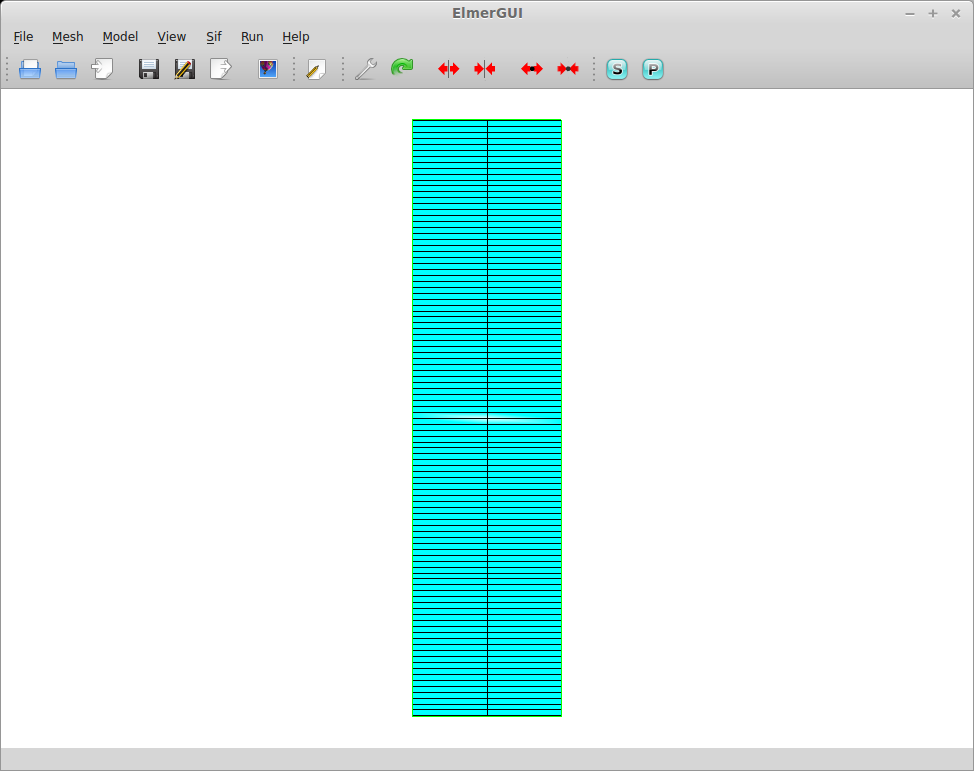
\includegraphics[width=100mm]{GeoSlabGeom}
\caption{The geometry of the mesh in ElmerGUI}\label{fg:geomesh}
\end{center}
\end{figure}

After we have the mesh we start to go through the Model menu from the top to bottom. 
In the \texttt{Setup} we choose things related to the whole simulation such as file names, 
time stepping, constants etc.
The simulation is carried out in 2-dimensional cartesian
coordinates and in transient. 
We will use 1000 timesteps each of size 10 years. 
For time-stepping we will use 2nd order scheme. 
\ttbegin
Model
  Setup 
    Simulation Type = Steady transient
    Timestepping Method = BDF
    Timestepping Order = 2 
    Timestep Intervals = 10000
    Timestep Sizes = $10*365*24*3600
    Output Intervals = 2
\ttend
Choose \texttt{Accept} to close the window.

In the equation section we choose the relevant equations and parameters related to their solution. 
In this case we'll have one set only one equation -- the heat equation.


When defining Equations and Materials it is possible to assign the to bodies immediately, or to use mouse
selection to assign them later. In this case we have just one body and one boundary and therefore its easier to assign 
the Equation and Material to it directly.

For the linear system solvers we are happy to use the defaults. One may however, try out different
preconditioners (ILU1,\ldots) or direct Umfpack solver, for example.
\ttbegin
Model
  Equation
    Add 
      Name = Heat Equation
      Apply to bodies = 1
      Heat Equation
        Active = on
  Apply   
  OK
\ttend        

The Material section includes all the material parameters.
They are divided to generic parameters which are direct properties of the material
without making any assumptions on the physical model, such as the mass. Other properties assume
a physical law, such heat conductivity.
\ttbegin
Model
  Material
    Add 
      Name = Granite
      Apply to bodies = 1 
      General    
        Density = 2700.0
        Heat Capacity = 1250.0
      Heat Equation
        Heat Conductivity = 2.5
    Apply
    OK
\ttend

We will need an initial condition for the case. 
\ttbegin
Model
  Initial Condition
    Add 
      Name = InitialState
      Heat Equation
        Temperature -> press enter and write the expression
      Apply to bodies = 1
    Apply
    OK
\ttend    
Now the expression to be written uses an internal linear interpolation feature of Elmer. 
\begin{verbatim}
Variable coordinate 2
  Real
    -8000 320.0
    -6500 260.0
    -6499 500.0
    -5501 500.0
    -5500 220.0
    -4000 160.0
  End
\end{verbatim}

In this case we only need boundary conditions for the upper and lower boundary.
First we create the boundary conditions
\ttbegin
Model
  BoundaryCondition
    Add 
      Heat Equation
        Temperature = 320.0
      Name = Down
      OK
    Add 
      Heat Equation
        Temperature = 160.0
      Name = Up
      OK
\ttend   
Then we set the boundary properties 
\ttbegin
Model 
  Set boundary properties  
\ttend
Choose the defined group of three boundaries by clicking with the mouse
and apply the condition for the lower boundary.
\ttbegin
Boundary condition
  Down
\ttend
and similarly for the upper boundary. 


For the execution 
ElmerSolver needs the mesh files and the command file. We have know basically defined
all the information for ElmerGUI to write the command file. After writing it we may also visually 
inspect the command file.
\ttbegin
Sif
  Generate
  Edit... -> look how your command file came out  
\ttend

Before we can execute the solver we should save the files in a directory. In saving the project all the
necessary files for restarting the case will be saved to the 
destination directory.
\ttbegin
File 
  Save Project
\ttend

After we have successfully saved the files we may start the solver
\ttbegin
Run
  Start solver
\ttend
A convergence view automatically pops up showing relative changes of each iteration.
As the case is linear only one iteration was required for the solution and the second one
just is needed to check the convergence. 
The resulting output log is shown in figure~\ref{fg:GeoSlabConv}.

\begin{figure}
\begin{center}
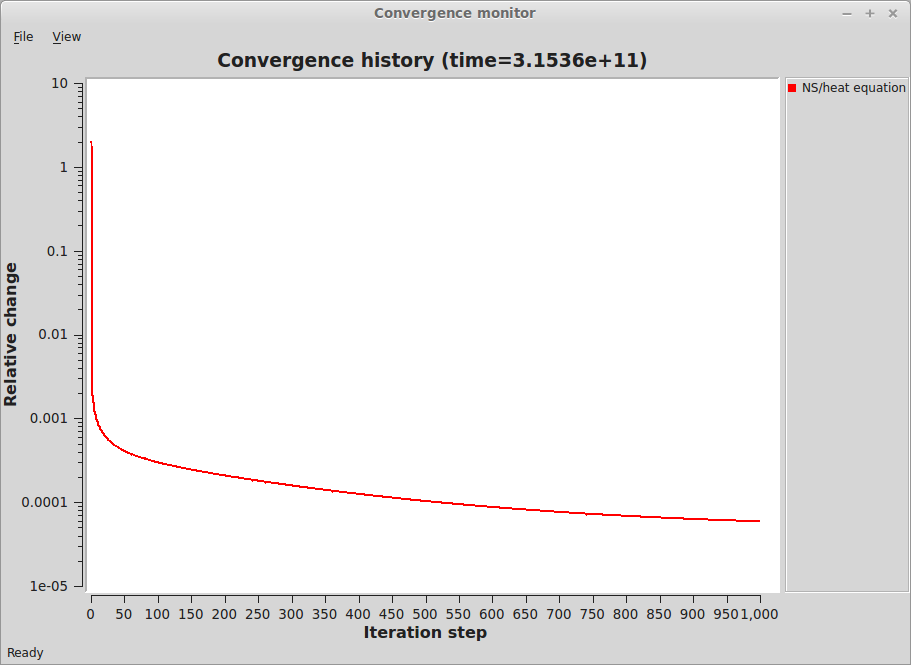
\includegraphics[width=100mm]{GeoSlabConvergence}
\caption{The output log of ElmerSolver when used under ElmerGUI}\label{fg:GeoSlabConv}
\end{center}
\end{figure}

Note: if you face problems in the solution phase and need to edit the setting, always remember to save
the project before execution.

To view the results we use Paraview.
\ttbegin
Run
  Start ParaView
\ttend
If your configuration is ok a Paraview window should pop up.
Choose temperature for the surface to be plotted. 
As we have a timeseries we may run the sequence by pressing the play icon. 

You may also choose the \texttt{Plot Over Line} filter to see the data plotted 
over a line for better numerical inspection. 

\begin{figure}
\begin{center}
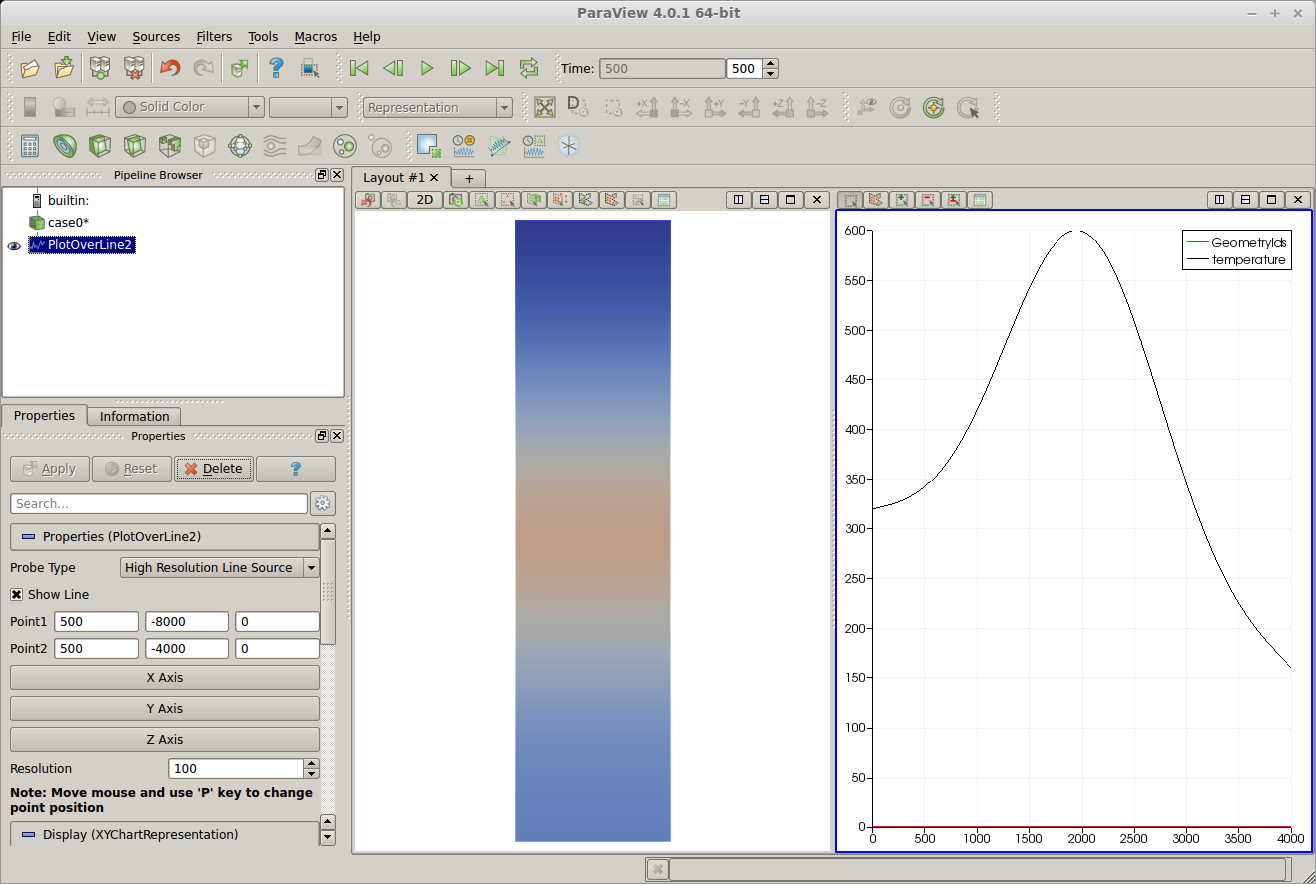
\includegraphics[width=140mm]{GeoSlabParaview}
\caption{The data visualized in Paraview as a surface and lineplot}
\label{fg:GeoSlabParaview}
\end{center}
\end{figure}

The final maximum temperature of the analysis is around 600~C. Whether this is close to correct could
be studied by increasing further the time and space resolution. 


\subsection{Variation accounting for latent heat release}

For intrusion processes the latent heat often plays on important role. 
For that the internal phase change model can be used. It requires that 
all the internal energy is expressed using specific enthalphy rather than
heat capacity and latent heat. 

We now eliminate the heat capacity of the original case (1250~J/kgK) and
create a specific enthalpy that includes heat capacity of 1000~J/kgJ 
and latent heat release of 200~kJ/kg release between interval 700--800 C.

The expression for \texttt{Specific Enthalpy} accounting for these two now yields
\begin{verbatim}
Variable Temperature
  Real
    0.0  0.0
    700  7.0e5
    800  9.0e5
    900  10.0e5
 End 
\end{verbatim}
For the phase change model we select 
\ttbegin
Model
  Equation
    Heat Equation
      Phase Change Model = spatial 2
  Update
  OK
\ttend        
With these changes the maximum temperature at the end of simulation cycle 
becomes around 624~C.  


\hfill
\mbox{}









%3D alternative
\graphicspath{{./}{TemperatureGeneric/}}
\chapter{Temperature distribution of a toy glacier}

\modinfo{Directory}{ToyGlacierTemperature}
\modinfo{Solvers}{\Idx{HeatSolver}} 
\modinfo{Tools}{\Idx{ElmerGUI},\Idx{nglib}} 
\modinfo{Dimensions}{2D, Steady-state}
\modinfo{Author}{Peter R{\aa}back, Thomas Zwinger}


\subsection*{Introduction}

The purpose of this simple tutorial is to be an introduction into Elmer for people dealing with computational glaceology.
This tutorial shows how to apply one equation and related boundary conditions to just one domain.


\subsection*{Problem description}

Consider a 2D toy model of a glacier with length of 7000~m and thickness of about 1000~m. 
There is a slight declination in the geometry which will make the glacier flow to the left. 
The left-hand-side is rounded to imitate a true glacier while the right-hand-side is 
cut off. 

\begin{figure}
\begin{center}
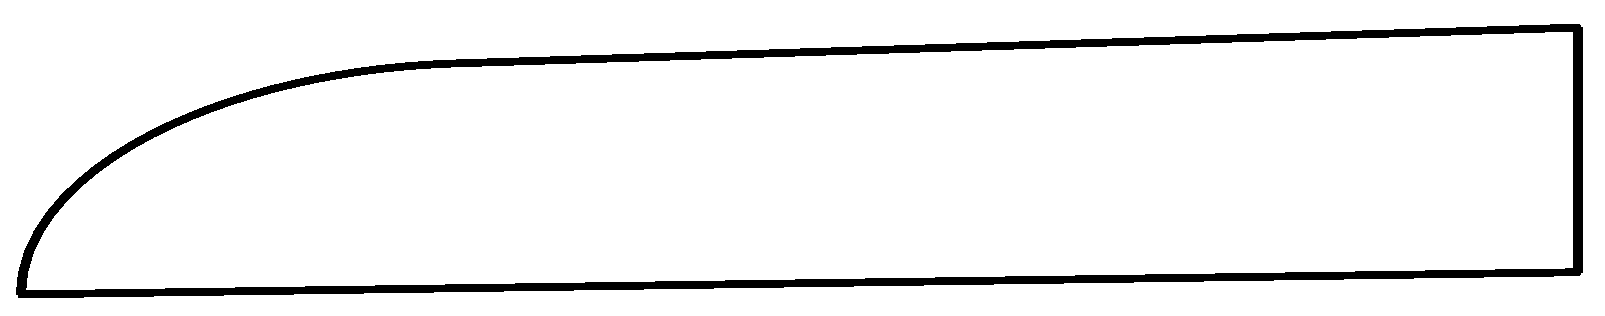
\includegraphics[width=120mm]{glacier_toy_shape}
\caption{The shape of the toy glacier to be studied}\label{glac:shape}
\end{center}
\end{figure}

We solve for the temperature distribution $T$ of the glacier. 
A heat flux of $q=0.02$~W/m$^2$ is applied at the bottom of the glacier while the surface stays at a
fixed temperature of $T_0=-10$~C. The material properties of ice are used for the 
heat conductivity $\kappa(T)$. 
The temperature distribution in the glacier 
may be solved from
\begin{equation}
\left \{
\begin{array}{cccc}
- \kappa \Delta T &= & 0 & \mathrm{ in } \, \, \Omega \\
T&=&T_0 & \mathrm{ on } \, \, \Gamma_D \\
\kappa \frac{\partial T}{\partial n} &=& q & \mathrm{ on } \,\, \Gamma_N \\
\end{array}
\right .
\end{equation}

\subsection*{Starting and meshing}

Start \texttt{ElmerGUI} from command line or by clicking the icon in your desktop (or in the /bin directory of you installation). 
Here we describe the essential steps in the ElmerGUI by writing out the clicking procedure. Tabulation generally means that the 
selections are done within the window chosen at the higher level. 

The mesh is given in ElmerGrid format in file \texttt{glacier\_toy.in2d} in the samples directory of ElmerGUI, 
load this file.
\ttbegin
File 
  Open -> glacier\_toy.in2d
\ttend
You should obtain a mesh consisting of just two triangular elements. The mesh is created by the \texttt{netgen} plugin 
and in order to increase the mesh density the in-line parameters of netgen must be defined in ElmerGUI.
Here we set the maximum element size to 50. 
\ttbegin
Mesh
  Configure... 
    nglib -> Max H: 50
\ttend
The resulting mesh should consist of 3335 nodes and 6355 triangles as may be checked in the 
\texttt{Model summary} window.
%If the mesh was successfully imported your window should look something in figure~\ref{glac:mesh}.

%\begin{figure}
%\begin{center}
%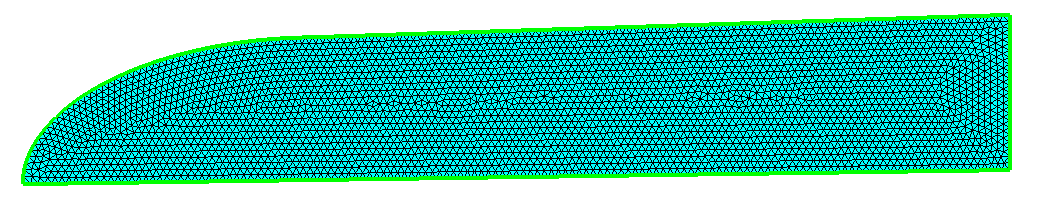
\includegraphics[width=120mm]{glacier_toy_mesh}
%\caption{The finite element mesh in ElmerGUI}\label{glac:mesh}
%\end{center}
%\end{figure}

\subsection*{Command file definition}

After we have the mesh we start to go through the Model menu from the top to bottom. 
In the \texttt{Setup} we choose things related to the whole simulation such as file names, 
time stepping, constants etc.
The simulation is carried out in 2-dimensional cartesian
coordinates and in steady-state. 
Only one steady-state iteration is needed as the case is linear. 
\ttbegin
Model
  Setup 
    Simulation Type = Steady state
    Steady state max. iter = 1
\ttend
Choose \texttt{Accept} to close the window.

In the equation section we choose the relevant equations and parameters related to their solution. 
In this case we'll have one set only one equation -- the heat equation.


When defining Equations and Materials it is possible to assign the to bodies immediately, or to use mouse
selection to assign them later. In this case we have just one body and one boundary and therefore its easier to assign 
the Equation and Material to it directly.

For the linear system solvers we are happy to use the defaults. One may however, try out different
preconditioners (ILU1,\ldots) or direct Umfpack solver, for example.
\ttbegin
Model
  Equation
    Add 
      Name = Heat Equation
      Apply to bodies = 1
      Heat Equation
        Active = on
  Apply   
  OK
\ttend        

The Material section includes all the material parameters.
They are divided to generic parameters which are direct properties of the material
without making any assumptions on the physical model, such as the mass. Other properties assume
a physical law, such heat conductivity.
We choose ice from the Material library which automatically sets for the needed material properties. 
\ttbegin
Model
  Material
    Add 
      Material library
        Water (frozen)
      Apply to bodies = Body 1 
      Add 
      OK
\ttend
This includes, for example, temperature dependent heat conductivity as may be seen under the HeatEquation page of
the material properties. MATC language is used here to define the functional form.


A Body Force represents the right-hand-side of a equation that in this case represents
the heat source. In this case there are no internal heat sources so we do not need one.
Also no Initial Condition is required in steady state case.

\begin{figure}
\begin{center}
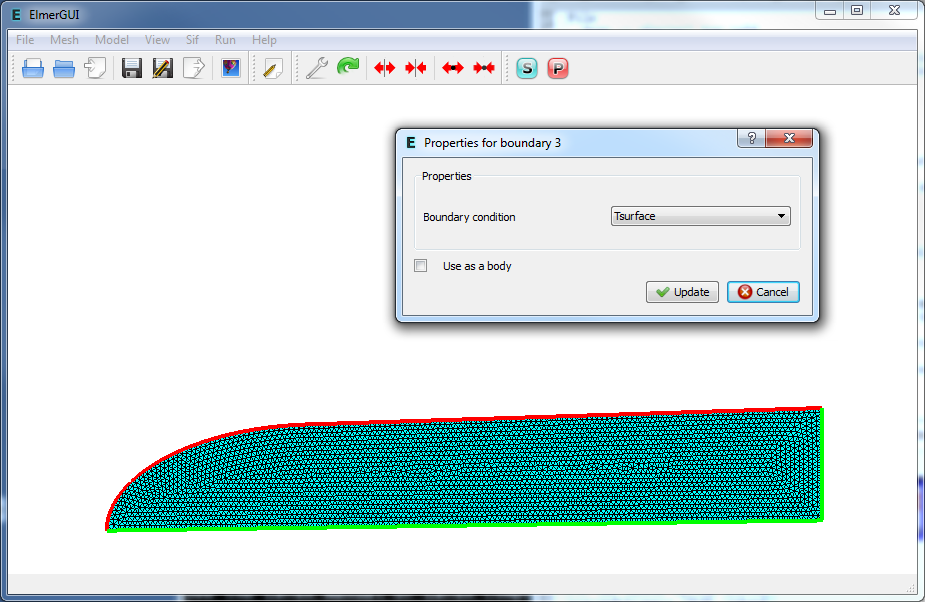
\includegraphics[width=120mm]{glacier_toy_gui}
\caption{Defining boundary conditions in ElmerGUI session}\label{glac:bc}
\end{center}
\end{figure}

We set three different kinds of boundary conditions. A fixed temperature, a fixed 
flux and natural boundary condition (zero flux). As there are several boundaries
we first define the different boundary types, and thereafter assign them using the mouse.
A screenshot of the case when setting the BCs is shown in figure~\ref{glac:bc}.

\ttbegin
Model
  BoundaryCondition
    Add 
      Heat Equation
        Temperature = -10.0
      Name = Tsurface
      OK
    Add 
      Heat Equation
        Heat Flux = 0.02
      Name = Tflux
      OK
    Add 
      Name = Tnatural
      OK
\ttend   
Then we set the boundary properties 
\ttbegin
Model 
  Set boundary properties  
\ttend
Choose the correct boundary by clicking with the mouse
and apply the condition for this boundary.
\ttbegin
Boundary condition
  Click top boundary -> choose Tsurface
  Click bottom boundary -> choose Tflux
  Click r.h.s. boundary -> choose Tnatural
\ttend

\subsection*{Saving and solution}

For the execution 
ElmerSolver needs the mesh files and the command file. We have know basically defined
all the information for ElmerGUI to write the command file. After writing it we may also visually 
inspect the command file.
\ttbegin
Sif 
  Generate
  Edit -> look how your command file came out  
\ttend

Before we can execute the solver we should save the files in a directory. In saving the project all the
necessary files for restarting the case will be saved to the 
destination directory.
\ttbegin
File 
  Save Project
\ttend

After we have successfully saved the files we may start the solver
\ttbegin
Run
  Start solver
\ttend
A convergence view automatically pops up showing relative changes of each iteration.
The heat conductivity of ice is set to be dependent on temperature and this results to a 
nonlinear iteration.
The resulting output is shown in figure~\ref{glac:conv}.

\begin{figure}
\begin{center}
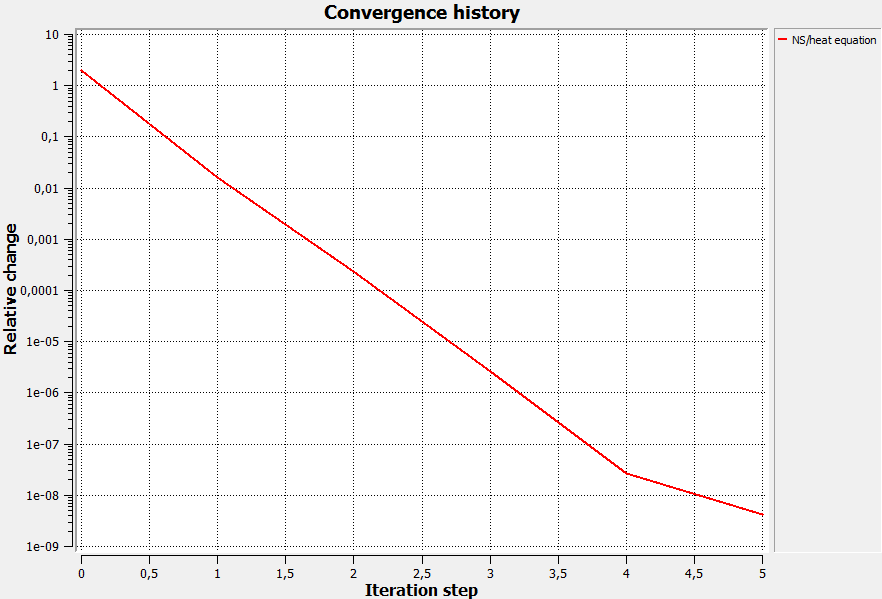
\includegraphics[width=100mm]{glacier_toy_convergence}
\caption{The convergence  ElmerGUI}\label{glac:conv}
\end{center}
\end{figure}

Note: if you face problems in the solution phase and need to edit the setting, always remember to save
the project before execution.

\subsection*{Results}

To view the results we use Paraview,
\ttbegin
Run
  Start Paraview
\ttend
Picture~\ref{glac:figtemp} shows
the surface mesh colored with temperature.
Note that these results were carried out with the obsolite
VTK based tool within ElmerGUI, and therefore look different than in Paraview.

\begin{figure}
\begin{center}
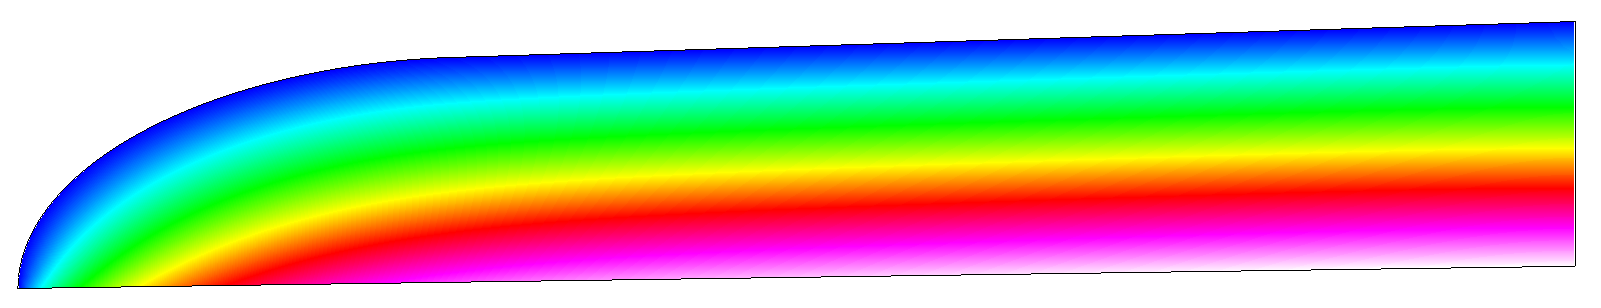
\includegraphics[width=120mm]{glacier_toy_temp}
\caption{The temperature distribution of the toy glacier.}\label{glac:figtemp}
\end{center}
\end{figure}


The maximum temperature obtained with the above choices is 0.11166~C. 
With a denser mesh the result is
naturally more accurate, but solving the problem takes more calculation time.

You may study the effect of mesh refinement by choosing 
a different value for the \texttt{Max H} parameter.
under \texttt{Configure}. After choosing \texttt{Remesh} and saving the mesh 
the solver may be recalled with the modified mesh.


\section*{Transient simulation}

We use the steady-state simulation presented above as our starting point and 
solve a transient version of it. Initially the glacier is assumed to be at -10~C 
and it is gradually heated from below. 


We use 2nd order bdf time-stepping method is selected with 100 steps
and with step size of 100 years - melting the ice from below with such a small flux 
would take quite a few years. 
The mathematical expression followed 
by ``\$'' is evaluated when the command file is read.
Here it is used to transform the time in years to those in one second. 
\ttbegin
Model
  Setup 
    Simulation Type = Transient
    Time Stepping Method = bdf
    BDF Order = 2
    Time Step Intervals = 100
    Time Step Sizes = \$ 3600 * 24 * 365.25 * 100
    Gravity = ...
\ttend

Initial conditions should be given to transient cases. In this case we choose a constant Temperature 
of -10~C. This is consistant with the boundary condition at the top wall.
\ttbegin
Model
  Initial Condition 
    Name = Initial Guess
    Heat Equation
      Temperature = -10.0
\ttend

\begin{figure}
\begin{center}
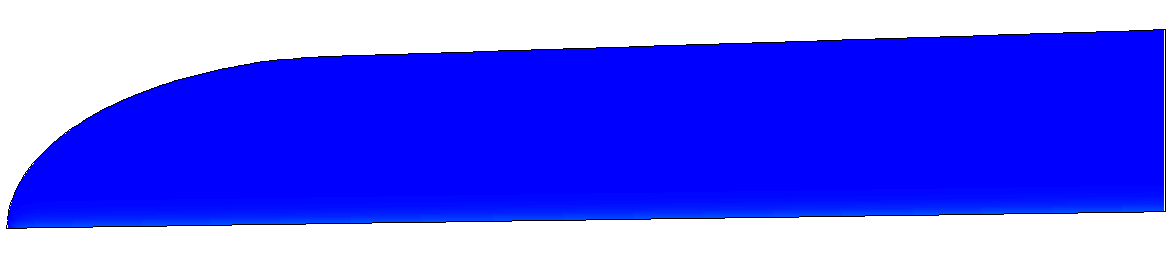
\includegraphics[width=120mm]{glacier_t1}
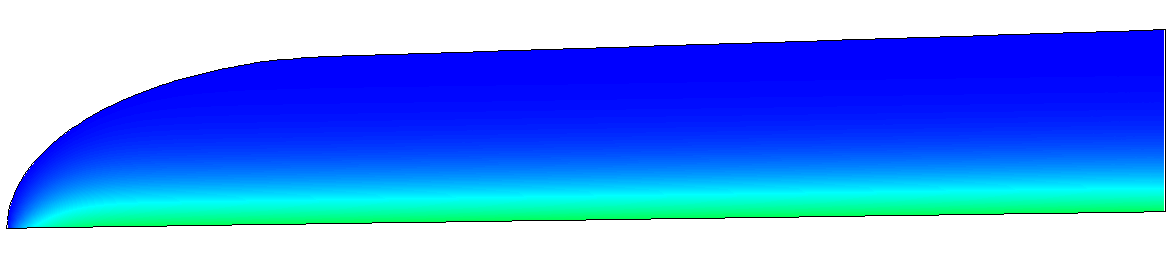
\includegraphics[width=120mm]{glacier_t20}
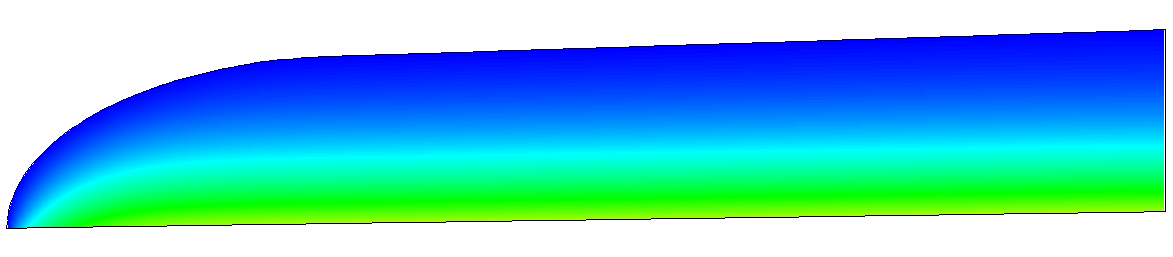
\includegraphics[width=120mm]{glacier_t50}
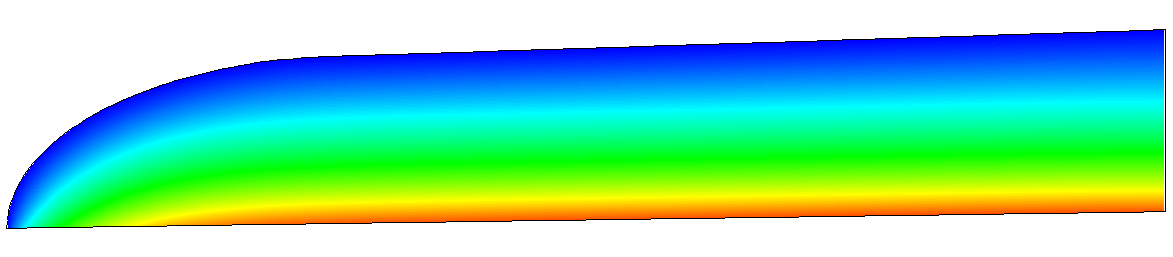
\includegraphics[width=120mm]{glacier_t100}
\caption{Temperature distribution after 1, 20, 50 and 100 timesteps. The temperature scale is the 
same that is used in the steady-state case. The maximum temperature at end should be about -3.7611~C.}
\end{center}
\end{figure}

\hfill
\mbox{}








%2D alternative
%\graphicspath{{./}{TemperatureAngleGUI/}}
%\chapter{Temperature distribution of a toy glacier}

\modinfo{Directory}{ToyGlacierTemperature}
\modinfo{Solvers}{\Idx{HeatSolver}} 
\modinfo{Tools}{\Idx{ElmerGUI},\Idx{nglib}} 
\modinfo{Dimensions}{2D, Steady-state}
\modinfo{Author}{Peter R{\aa}back, Thomas Zwinger}


\subsection*{Introduction}

The purpose of this simple tutorial is to be an introduction into Elmer for people dealing with computational glaceology.
This tutorial shows how to apply one equation and related boundary conditions to just one domain.


\subsection*{Problem description}

Consider a 2D toy model of a glacier with length of 7000~m and thickness of about 1000~m. 
There is a slight declination in the geometry which will make the glacier flow to the left. 
The left-hand-side is rounded to imitate a true glacier while the right-hand-side is 
cut off. 

\begin{figure}
\begin{center}
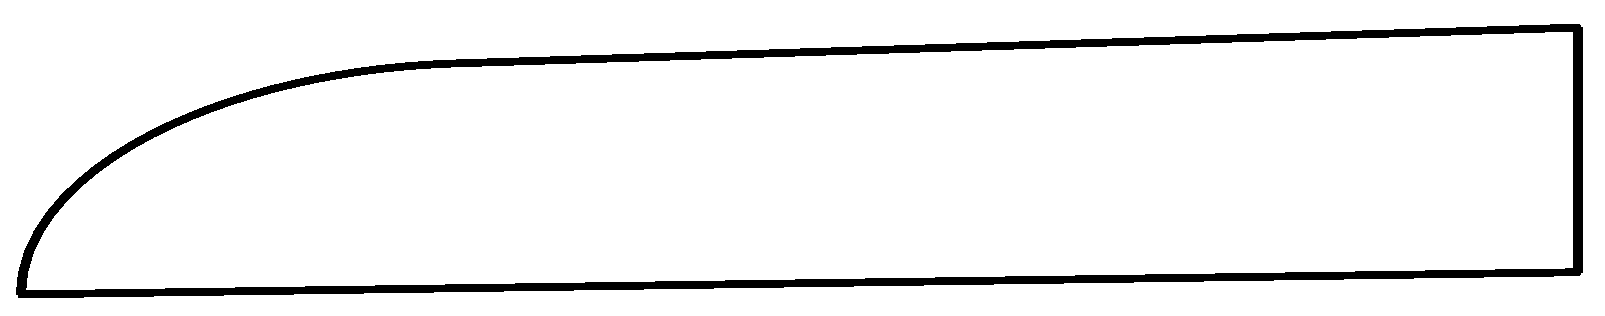
\includegraphics[width=120mm]{glacier_toy_shape}
\caption{The shape of the toy glacier to be studied}\label{glac:shape}
\end{center}
\end{figure}

We solve for the temperature distribution $T$ of the glacier. 
A heat flux of $q=0.02$~W/m$^2$ is applied at the bottom of the glacier while the surface stays at a
fixed temperature of $T_0=-10$~C. The material properties of ice are used for the 
heat conductivity $\kappa(T)$. 
The temperature distribution in the glacier 
may be solved from
\begin{equation}
\left \{
\begin{array}{cccc}
- \kappa \Delta T &= & 0 & \mathrm{ in } \, \, \Omega \\
T&=&T_0 & \mathrm{ on } \, \, \Gamma_D \\
\kappa \frac{\partial T}{\partial n} &=& q & \mathrm{ on } \,\, \Gamma_N \\
\end{array}
\right .
\end{equation}

\subsection*{Starting and meshing}

Start \texttt{ElmerGUI} from command line or by clicking the icon in your desktop (or in the /bin directory of you installation). 
Here we describe the essential steps in the ElmerGUI by writing out the clicking procedure. Tabulation generally means that the 
selections are done within the window chosen at the higher level. 

The mesh is given in ElmerGrid format in file \texttt{glacier\_toy.in2d} in the samples directory of ElmerGUI, 
load this file.
\ttbegin
File 
  Open -> glacier\_toy.in2d
\ttend
You should obtain a mesh consisting of just two triangular elements. The mesh is created by the \texttt{netgen} plugin 
and in order to increase the mesh density the in-line parameters of netgen must be defined in ElmerGUI.
Here we set the maximum element size to 50. 
\ttbegin
Mesh
  Configure... 
    nglib -> Max H: 50
\ttend
The resulting mesh should consist of 3335 nodes and 6355 triangles as may be checked in the 
\texttt{Model summary} window.
%If the mesh was successfully imported your window should look something in figure~\ref{glac:mesh}.

%\begin{figure}
%\begin{center}
%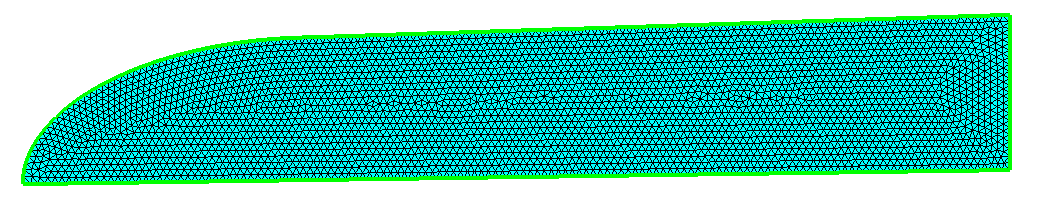
\includegraphics[width=120mm]{glacier_toy_mesh}
%\caption{The finite element mesh in ElmerGUI}\label{glac:mesh}
%\end{center}
%\end{figure}

\subsection*{Command file definition}

After we have the mesh we start to go through the Model menu from the top to bottom. 
In the \texttt{Setup} we choose things related to the whole simulation such as file names, 
time stepping, constants etc.
The simulation is carried out in 2-dimensional cartesian
coordinates and in steady-state. 
Only one steady-state iteration is needed as the case is linear. 
\ttbegin
Model
  Setup 
    Simulation Type = Steady state
    Steady state max. iter = 1
\ttend
Choose \texttt{Accept} to close the window.

In the equation section we choose the relevant equations and parameters related to their solution. 
In this case we'll have one set only one equation -- the heat equation.


When defining Equations and Materials it is possible to assign the to bodies immediately, or to use mouse
selection to assign them later. In this case we have just one body and one boundary and therefore its easier to assign 
the Equation and Material to it directly.

For the linear system solvers we are happy to use the defaults. One may however, try out different
preconditioners (ILU1,\ldots) or direct Umfpack solver, for example.
\ttbegin
Model
  Equation
    Add 
      Name = Heat Equation
      Apply to bodies = 1
      Heat Equation
        Active = on
  Apply   
  OK
\ttend        

The Material section includes all the material parameters.
They are divided to generic parameters which are direct properties of the material
without making any assumptions on the physical model, such as the mass. Other properties assume
a physical law, such heat conductivity.
We choose ice from the Material library which automatically sets for the needed material properties. 
\ttbegin
Model
  Material
    Add 
      Material library
        Water (frozen)
      Apply to bodies = Body 1 
      Add 
      OK
\ttend
This includes, for example, temperature dependent heat conductivity as may be seen under the HeatEquation page of
the material properties. MATC language is used here to define the functional form.


A Body Force represents the right-hand-side of a equation that in this case represents
the heat source. In this case there are no internal heat sources so we do not need one.
Also no Initial Condition is required in steady state case.

\begin{figure}
\begin{center}
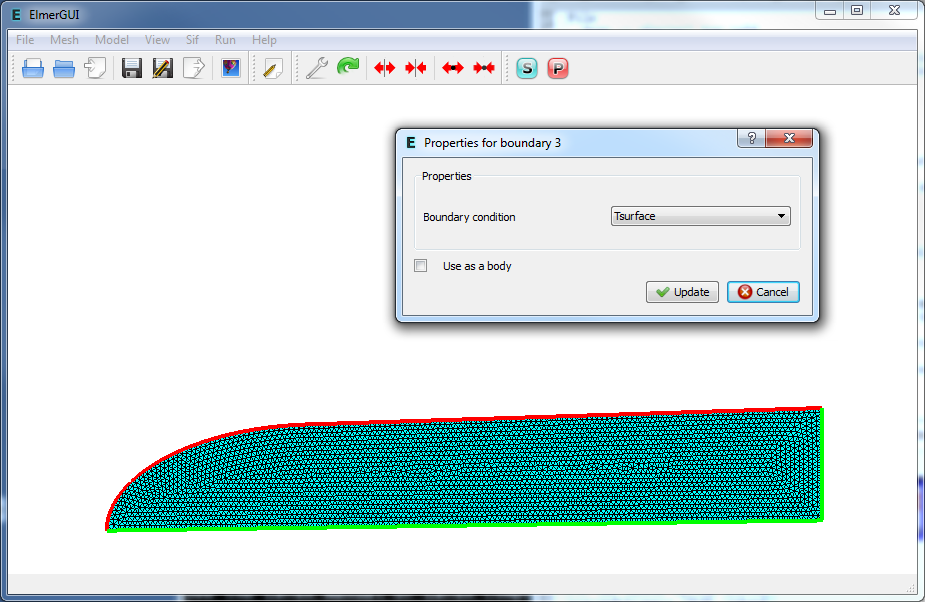
\includegraphics[width=120mm]{glacier_toy_gui}
\caption{Defining boundary conditions in ElmerGUI session}\label{glac:bc}
\end{center}
\end{figure}

We set three different kinds of boundary conditions. A fixed temperature, a fixed 
flux and natural boundary condition (zero flux). As there are several boundaries
we first define the different boundary types, and thereafter assign them using the mouse.
A screenshot of the case when setting the BCs is shown in figure~\ref{glac:bc}.

\ttbegin
Model
  BoundaryCondition
    Add 
      Heat Equation
        Temperature = -10.0
      Name = Tsurface
      OK
    Add 
      Heat Equation
        Heat Flux = 0.02
      Name = Tflux
      OK
    Add 
      Name = Tnatural
      OK
\ttend   
Then we set the boundary properties 
\ttbegin
Model 
  Set boundary properties  
\ttend
Choose the correct boundary by clicking with the mouse
and apply the condition for this boundary.
\ttbegin
Boundary condition
  Click top boundary -> choose Tsurface
  Click bottom boundary -> choose Tflux
  Click r.h.s. boundary -> choose Tnatural
\ttend

\subsection*{Saving and solution}

For the execution 
ElmerSolver needs the mesh files and the command file. We have know basically defined
all the information for ElmerGUI to write the command file. After writing it we may also visually 
inspect the command file.
\ttbegin
Sif 
  Generate
  Edit -> look how your command file came out  
\ttend

Before we can execute the solver we should save the files in a directory. In saving the project all the
necessary files for restarting the case will be saved to the 
destination directory.
\ttbegin
File 
  Save Project
\ttend

After we have successfully saved the files we may start the solver
\ttbegin
Run
  Start solver
\ttend
A convergence view automatically pops up showing relative changes of each iteration.
The heat conductivity of ice is set to be dependent on temperature and this results to a 
nonlinear iteration.
The resulting output is shown in figure~\ref{glac:conv}.

\begin{figure}
\begin{center}
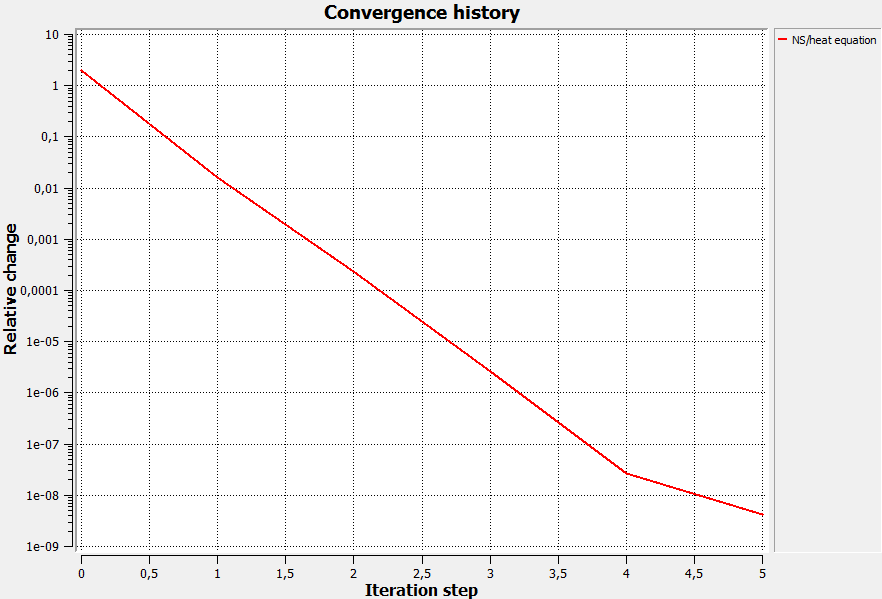
\includegraphics[width=100mm]{glacier_toy_convergence}
\caption{The convergence  ElmerGUI}\label{glac:conv}
\end{center}
\end{figure}

Note: if you face problems in the solution phase and need to edit the setting, always remember to save
the project before execution.

\subsection*{Results}

To view the results we use Paraview,
\ttbegin
Run
  Start Paraview
\ttend
Picture~\ref{glac:figtemp} shows
the surface mesh colored with temperature.
Note that these results were carried out with the obsolite
VTK based tool within ElmerGUI, and therefore look different than in Paraview.

\begin{figure}
\begin{center}
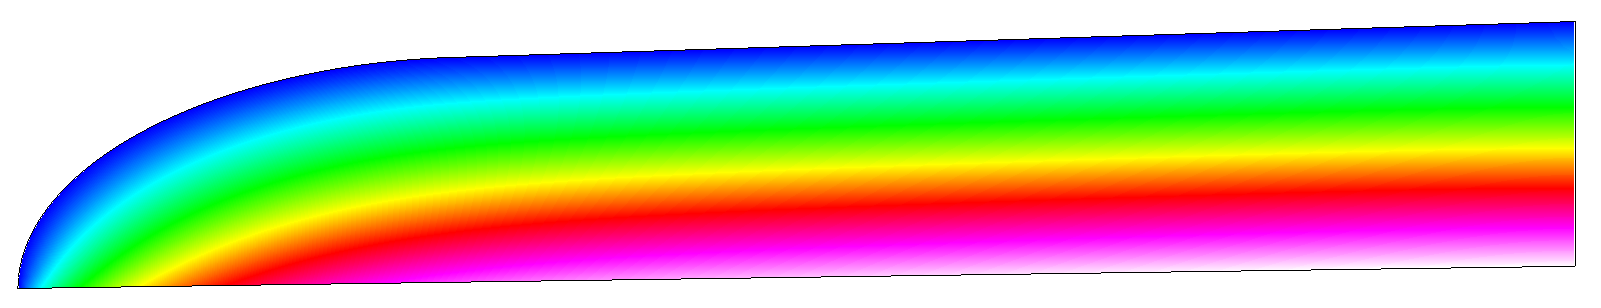
\includegraphics[width=120mm]{glacier_toy_temp}
\caption{The temperature distribution of the toy glacier.}\label{glac:figtemp}
\end{center}
\end{figure}


The maximum temperature obtained with the above choices is 0.11166~C. 
With a denser mesh the result is
naturally more accurate, but solving the problem takes more calculation time.

You may study the effect of mesh refinement by choosing 
a different value for the \texttt{Max H} parameter.
under \texttt{Configure}. After choosing \texttt{Remesh} and saving the mesh 
the solver may be recalled with the modified mesh.


\section*{Transient simulation}

We use the steady-state simulation presented above as our starting point and 
solve a transient version of it. Initially the glacier is assumed to be at -10~C 
and it is gradually heated from below. 


We use 2nd order bdf time-stepping method is selected with 100 steps
and with step size of 100 years - melting the ice from below with such a small flux 
would take quite a few years. 
The mathematical expression followed 
by ``\$'' is evaluated when the command file is read.
Here it is used to transform the time in years to those in one second. 
\ttbegin
Model
  Setup 
    Simulation Type = Transient
    Time Stepping Method = bdf
    BDF Order = 2
    Time Step Intervals = 100
    Time Step Sizes = \$ 3600 * 24 * 365.25 * 100
    Gravity = ...
\ttend

Initial conditions should be given to transient cases. In this case we choose a constant Temperature 
of -10~C. This is consistant with the boundary condition at the top wall.
\ttbegin
Model
  Initial Condition 
    Name = Initial Guess
    Heat Equation
      Temperature = -10.0
\ttend

\begin{figure}
\begin{center}
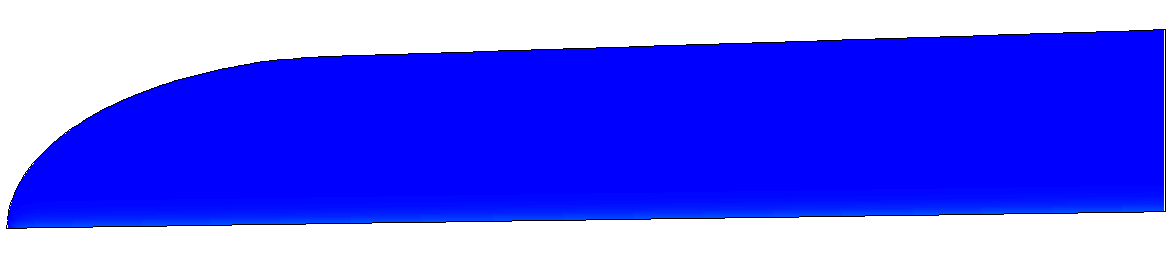
\includegraphics[width=120mm]{glacier_t1}
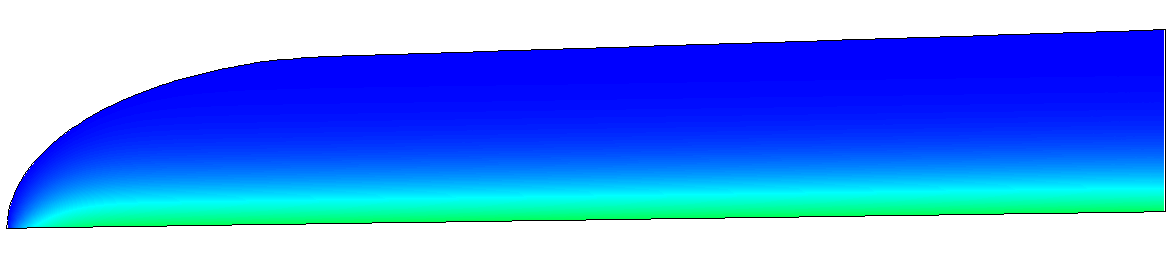
\includegraphics[width=120mm]{glacier_t20}
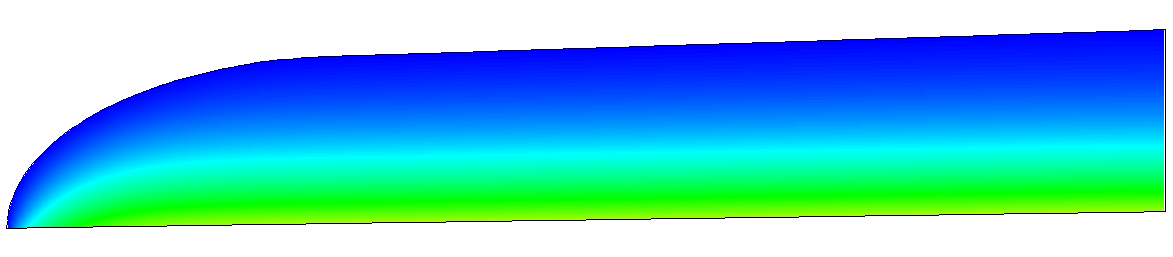
\includegraphics[width=120mm]{glacier_t50}
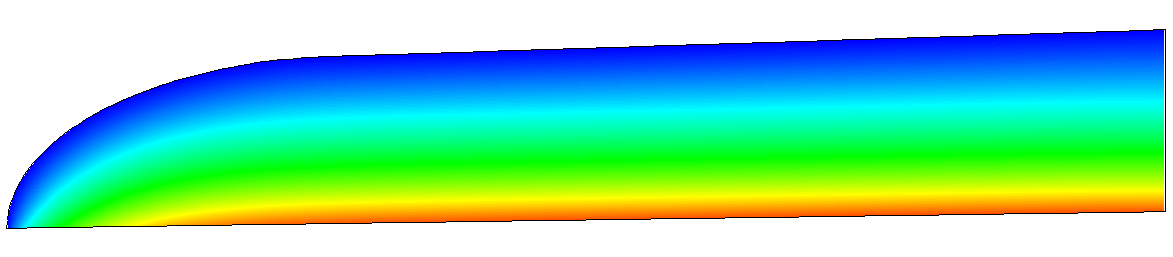
\includegraphics[width=120mm]{glacier_t100}
\caption{Temperature distribution after 1, 20, 50 and 100 timesteps. The temperature scale is the 
same that is used in the steady-state case. The maximum temperature at end should be about -3.7611~C.}
\end{center}
\end{figure}

\hfill
\mbox{}








%2D
%\graphicspath{{./}{ElasticBeamGUI/}}
%\chapter{Linear elasticity equation -- Loaded elastic beam -- 2D}

\modinfo{Directory}{ElasticBeamGUI}
\modinfo{Solvers}{\Idx{StressSolve}}
\modinfo{Tools}{\Idx{ElmerGUI}}
\modinfo{Dimensions}{2D, Steady-state}
\modinfo{Author}{Peter R{\aa}back}


\subsection*{Case definition}

A homogenous, elastic beam ($\Omega$) is rigidly supported on one 
end (boundary $\Gamma_4$). On boundary $\Gamma_3$ the beam is subjected 
to a load $q(x)$, which grows linearly from zero to $q_0$ 
(see figure~\ref{fg:beam}). The length of the beam is 1~m and the thickness 0.1~m.
Material properties of the beam are those of iron (in the database) Poisson 
ratio 0.29 and Young's modulus $193\cdot 10^9$N/m$^2$. Problem is to solve the 
displacement of the beam.  

\begin{figure}[h]
\centering
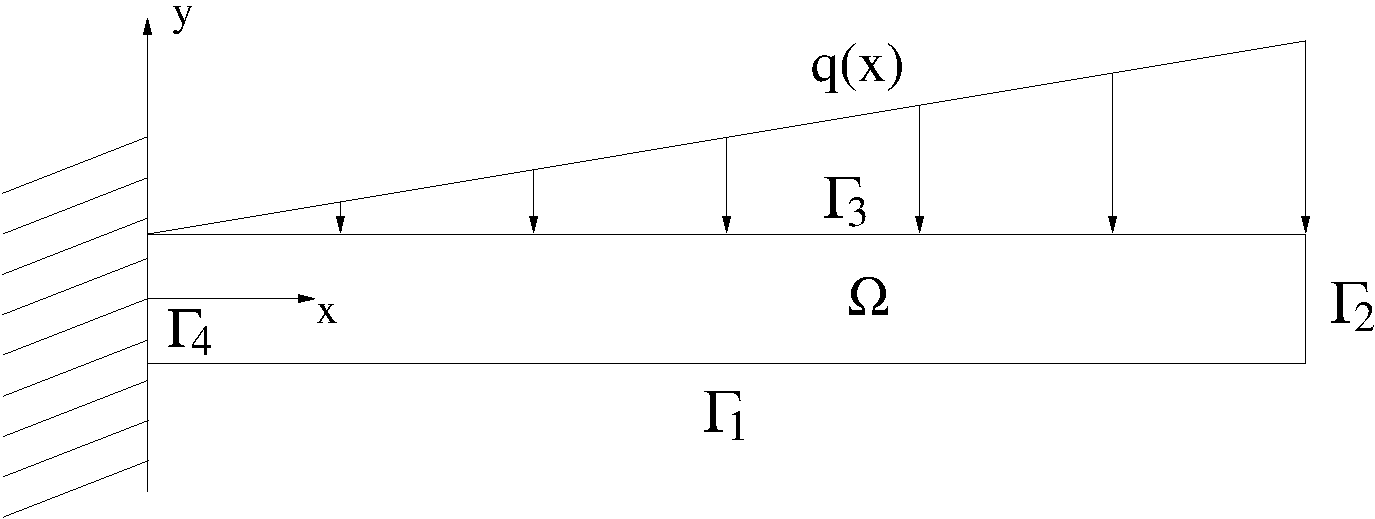
\includegraphics[width=100mm]{Beam}
\caption{Beam and loading.}\label{fg:beam}
\end{figure}

Problem is solved according to linear elasticity theory. Mathematically 
the problem to be solved is
\begin{equation}
\left \{
\begin{array}{rcll}
-div \sigma & = & 0 & \mbox{ in } \Omega \\
\sigma & = & \lambda tr [\varepsilon(u)]I + 2 \mu \varepsilon(u) &
\mbox{ in } \Omega \\
u & = & 0 & \mbox{ on } \Gamma_4 \\
\sigma n & = & 0 & \mbox{ on } \Gamma_1 \cup \Gamma_2 \\
\sigma n & = & -q & \mbox{ on } \Gamma_3 \\
\end{array}
\right .
\end{equation}
where $\lambda$ and $\mu$ are the Lam\'{e} constants (which can be expressed 
in terms of the Poisson ratio and Young's modulus), $\varepsilon$ is the 
linearised strain tensor, $u$ is the displacement vector, $q$ is the given
surface traction and $n$ is the outward unit normal to the boundary.



\subsection*{Solution procedure}

The mesh is given in ElmerGrid format in file \texttt{beam.grd}, load this file.
\ttbegin
File 
  Open -> beam.grd
\ttend
You should obtain your mesh and may check that it consists of 1000 biquadratic elements.
\begin{figure}[h!]
\begin{center}
  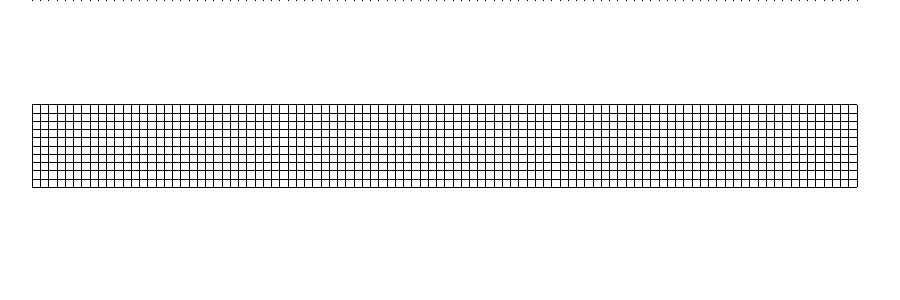
\includegraphics[width=0.8\textwidth,viewport=0 30 900 270,clip]{beammesh}
  \caption{The mesh used in the computations}
  \label{fig:elast_mesh}
\end{center}
\end{figure}

After we have the mesh we start to go through the Model menu from the top to bottom. 
In the Setup we choose things related to the whole simulation such as file names, 
time stepping, constants etc.
The simulation is carried in steady-state in 2-dimensional Cartesian
coordinates. 
\ttbegin
Model
  Setup 
    Simulation Type = Steady state
    Steady state max. iter = 1
\ttend

In the Equation section we choose the relevant equations which in this case only includes 
the \texttt{Linear elasticity} equation
which solves the problem according to 
linear elastic theory.
In this case we assume that the beam is thin in the $z$-direction and hence assume plane stresses.
When defining Equations and Materials it is possible to assign to the bodies immediately, or to use mouse
selection to assign them later. In this case we have just one body and therefore its easier to assign 
the Equation and Material to it directly.
For the linear system solvers we are happy to use the defaults. One may however, try out different
preconditioners (ILU1,\ldots) or direct Umfpack solver, for example.
\ttbegin
Model
  Equation
    Name = Elasticity
    Apply to Bodies = 1
    Linear elasticity
      Active = on
      Plane Stress = True
    Add 
    OK
\ttend        
The Material section includes all the material parameters.
They are divided to generic parameters which are direct properties of the material
without making any assumptions on the physical model, such as the mass. Other properties assume
a physical law, such as conductivities and viscosity. 

Here we choose the generic iron from the material library.
You may click through the material parameters of the various solvers to ensure that
the properties are indeed as they should be. Any consistent set of units may be used in Elmer.
The natural choice is of course to perform the computations in SI units. 

\ttbegin
Model
  Material
    Material library    
      Iron (generic)
    Apply to Bodies = 1 
    Add
    OK
\ttend

There are no body forces and convergence should be easily obtained with the default 
initial condition i.e. zero for all fields.

The first boundary condition fixes the beam rigidly at the wall.
The second boundary condition may seem confusing. Basically it represents the form 
using a linear interpolation between two points. At $x=0$ the force $f_y = 0$ and 
at $x=1$ the force $f_y=-1.0e7$, respectively. The semicolon is an alternative separator
to line break. To fill in the second boundary condition press \texttt{Enter} in the 
\texttt{Force 2} checkbox.
\ttbegin
Model
  BoundaryCondition
    Name = Wall
    Linear elasticity
      Displacement 1 = 0.0
      Displacement 2 = 0.0
    Add
    New

    Name = Top
    Linear elasticity 
      Force 2 = Variable Coordinate 1; Real; 0 0; 1 -1.0e7; End
    Add 
\ttend   

The conditions may also be assigned to boundaries in the Boundary condition menu, or 
by clicking with the mouse. Here we use the latter approach as that spares us of the 
need to know the indexes of each boundary.
\ttbegin
Model
  Set boundary properties
    Choose left-hand-side -> set boundary condition Wall
    Choose top -> set boundary condition Top
\ttend

For the execution 
ElmerSolver needs the mesh files and the command file. We have now basically defined
all the information for ElmerGUI to write the command file. After writing it we may also visually 
inspect the command file.
\ttbegin
Sif 
  Generate
  Edit -> look how your command file came out  
\ttend

Before we can execute the solver we should save the files in a directory. The project includes
all the files needed to restart the case.
\ttbegin
File 
  Save Project
\ttend

After we have successfully saved the files we may start the solver
\ttbegin
Run
  Start solver
\ttend
A convergence view automatically pops up showing relative changes of each iteration.
Two iterations are performed, the second one only to ensure convergence at the nonlinear level.
The norm of the finished computation should be around 0.01808.

When there are some results to view we may start the postprocessor also
\ttbegin
Run
  Start ParaView
\ttend


\subsection*{Results}

As a result the absolute value of maximum displacement is given. The 
displacements calculated with different load values $q_0$ are tabulated in 
table~\ref{tb:struct3a}. Note that the absolute value of the
displacement varies linearly with respect to the load since the model
is linear.

\begin{figure}[h!]
\begin{center}
  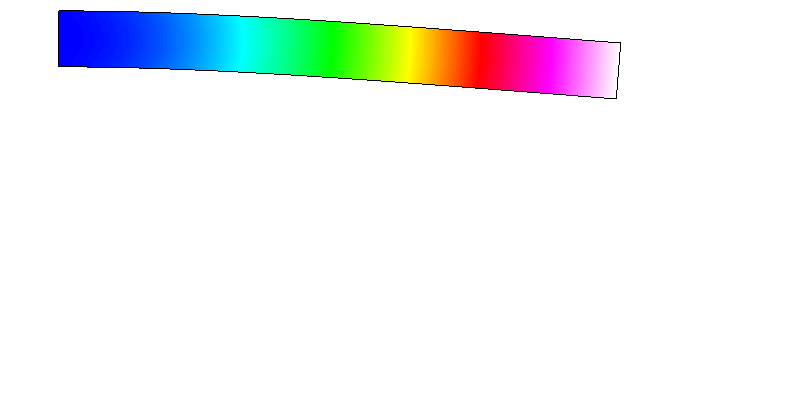
\includegraphics[width=0.4\textwidth,angle=0]{beam1.png}
  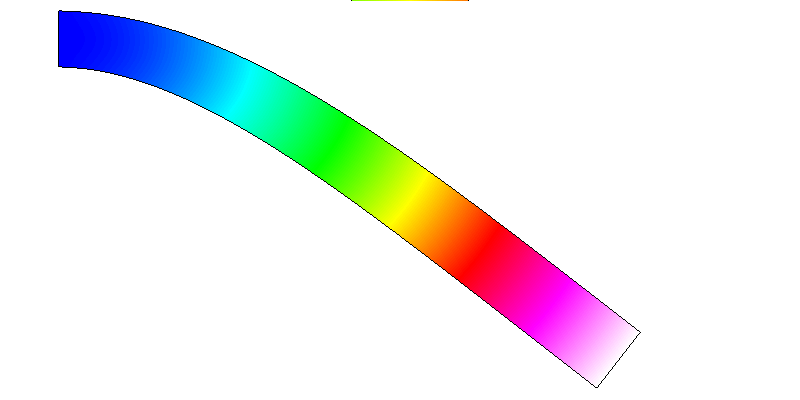
\includegraphics[width=0.4\textwidth,angle=0]{beam2.png}
  \caption{The displacement of an elastic beam with two different loads
using a linear model}
  \label{fig:elast_beam1}
\end{center}
\end{figure}

\begin{table}[h]
\caption{Displacements with different load values}
\label{tb:struct3a}
\begin{center}
\begin{tabular}{ll} \hline
$q_0$ [N/m$^2$] & $\max |u|$ [m] \\ \hline
-1.0$e7$ & 0.05755 \\
-1.0$e8$ & 0.5755 \\
-1.0$e9$ & 5.755 \\ \hline
\end{tabular}
\end{center}
\end{table}

If you look at the results you can see that the displacement values
become relatively large. The linear theory is valid only to small 
displacements. From Fig~\ref{fig:elast_beam1} you can also notice that the
beam does not maintain its original form. This means that the linear 
elasticity theory can not take into consideration all the necessary 
phenomena that are related to the problem, any more. To be able to 
solve the problem we must use general elasticity theory.


\subsection*{Extra task: transient loading}

If you have time you may try to solve the case using transient loading. 
You may try with the following settings.
\ttbegin
Model
  Setup 
    Simulation Type = Transient
    Time Stepping Method = bdf
    BDF Order = 2
    Time Step Intervals = 200
    Time Step Sizes = 1.0e-4
\ttend
Having a too large time step will not accurately describe the transient behaviour while having a too 
small time step consumes unnecessary resources. There is only numerical damping in the system and 
hence it will oscillate for some time.
%To visualize the oscillations set in the \texttt{Time Step Control} 
%in the \texttt{Do after frame} box the following command
%\ttbegin
%  math nodes=n0+Displacement(0:2,time($t))
%\ttend
%It will add the right timestep of the displacement field to the initial coordinate values.

 

\vfill
\mbox{}


\graphicspath{{./}{ModelPDE3D/}}
\chapter{Generic scalar PDE on 3D angle domain}

\modinfo{Directory}{ModelPDE3D}
\modinfo{Solvers}{\Idx{ModelPDE}} 
\modinfo{Tools}{\Idx{ElmerGUI}} 
\modinfo{Dimensions}{3D, Steady-state}
\modinfo{Author}{Peter R{\aa}back}


\subsection*{Problem description}

This tutorial demonstrates the use of the generic advection-diffusion-reaction 
equation through ElmerGUI. The solver may be found in module ModelPDE. 
The purposes of the model pde and also this tutorial is to help 
those who want to understand Elmer from a mathematical perspective to be
able to carry some own code development. 

The problem is a simple 3d structure \texttt{winkel.grd} that can be charectized by a 
$2\times 2\times 2$ topological grid where entries $(1,1,1)$, $(1,2,1)$, $(2,1,1)$ and
$(2,1,2)$ are meshed. This is the simplest cartesian structure with full 3D 
solution. 

We can rather freely play with the parameters of the Model PDE. The equation is 
generic and the parameters are assumed to be unit free. 
For detailed description of the problem see the description in Elmer Programmers Tutorial.

As a first suggestion, we will show how to make a simple case where the two extreme edges 
are set to zero using Dirichlet boundary conditions, and constant unity source term is 
applied to the body. This is the simple Poisson equation with constant coefficient. 

\subsection*{Menu structures for Model PDE}

The menu structures for the case are defined in \texttt{model-pde.xml}. If after starting
you cannot find the menu structures add the file to the \texttt{edf} directory of your installation,
or append the menu structures within ElmerGUI. 

\noindent 
The following material parameters may be defined
\sifbegin
\sifitem{Diffusion Coefficient}{Real}
Diffusion coefficient, $\mu$.
\sifitem{Reaction Coefficient}{Real}
Reaction coefficient, $\lambda$.
\sifitem{Time Derivative Coefficient}{Real}
Multiplier of the time derivative, $\rho$.
\sifitem{Convection Coefficient}{Real}
Multiplier of convection coefficient, $\kappa$.
\sifitem{Convection Velocity 1}{Real}
Convection velocity in direction $x$, $a_x$.
\sifitem{Convection Velocity 2}{Real}
Convection velocity in direction $y$, $a_y$.
\sifitem{Convection Velocity 3}{Real}
Convection velocity in direction $z$, $a_z$.
\sifend

\noindent
The following parameter defines the heat source $f$ on the right-hand-side
\sifbegin
\sifitemnt{Field Source}{Real}
\sifend

\noindent
The menu structures defines the following parameters for boundary conditions:
\sifbegin
\sifitem{Field}{Real}
Dirichlet BC for the scalar field under study, $u$.
\sifitem{Field Flux}{Real}
Neumann boundary condition for the field, $q$.
\sifitemnt{Robin Coeffficient}{Real}
\sifitem{External Field}{Real}
Coefficient $\alpha$ and external field value $g$ for Robin boundary condition.
\sifend

\noindent
In transient cases the user may also give an initial condition for $u$, 
\sifbegin
\sifitemnt{Field}{Real}
\sifend


\subsection*{Solution procedure}

Start \texttt{ElmerGUI} from command line or by clicking the icon in your desktop. Here we describe 
the essential steps in the ElmerGUI by writing out the clicking procedure. Tabulation generally means that the selections are done within the window chosen at the higher level. 

The mesh is given in ElmerGrid format in file \texttt{winkel.grd} in the samples directory of ElmerGUI, 
load this file.
\ttbegin
File 
  Open -> winkel.grd
\ttend
You should obtain your mesh and may check in the \texttt{Model summary} 
window that it consists of 35\,721 nodes and 32\,000 trilinear elements.
If the mesh was successfully imported your window should look something in figure~\ref{fg:modelpde1}.
The figure also shows the two extreme boundary patches that we intend to use Dirichlet conditions
for. 
\begin{figure}
\begin{center}
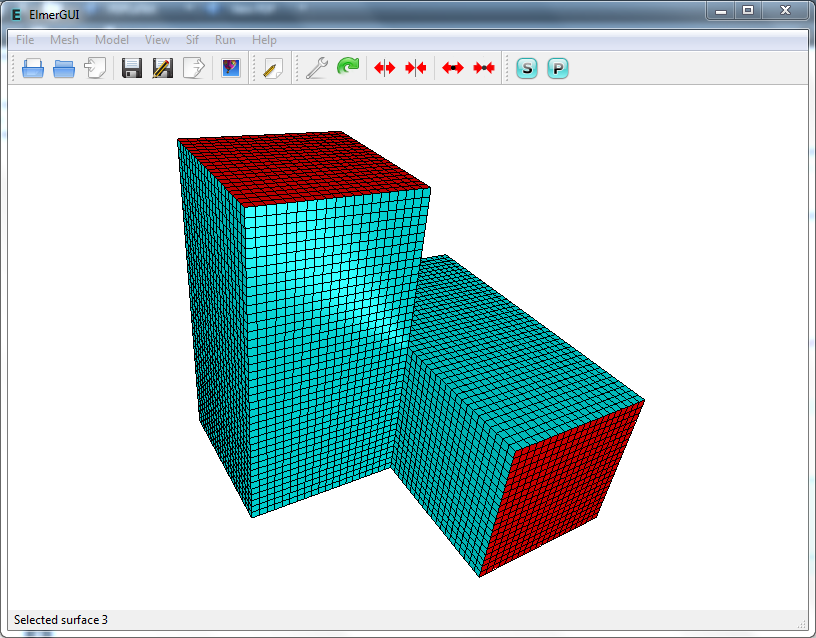
\includegraphics[width=100mm]{ModelPDE_Mesh.PNG}
\caption{The finite element mesh in ElmerGUI}\label{fg:modelpde1}
\end{center}
\end{figure}

After we have the mesh we start to go through the Model menu from the top to bottom. 
In the \texttt{Setup} we choose things related to the whole simulation such as file names, 
time stepping, constants etc.
The simulation is carried out in 2-dimensional cartesian
coordinates and in steady-state. 
Only one steady-state iteration is needed as the case is linear. 
\ttbegin
Model
  Setup 
    Simulation Type = Steady state
    Steady state max. iter = 1
\ttend
Choose \texttt{Accept} to close the window.

In the equation section we choose the relevant equations and parameters related to their solution. 
In this case we'll have one set only one equation -- the Model PDE.


When defining Equations and Materials it is possible to assign the to bodies immediately, or to use mouse
selection to assign them later. In this case we have just one body and one boundary and therefore its easier to assign 
the Equation and Material to it directly.

For the linear system solvers we are happy to use the defaults. One may however, try out different
preconditioners (ILU1,\ldots) or direct Umfpack solver, for example.
\ttbegin
Model
  Equation
    Add 
      Name = Model PDE
      Apply to bodies = 1
      Model PDE
        Active = on
  Apply   
  OK
\ttend        

The Material section includes all the material parameters.
If material parameter is not defined. It is assumed to be zero. 
Here we just set the diffusivity to one.
\ttbegin
Model
  Material
    Add 
      Name = Ideal
      Apply to bodies = 1 
      Model PDE
        Diffusion Coefficient = 1.0
    Apply
    OK
\ttend

A Body Force represents the right-hand-side of a equation,  
\ttbegin
Model
  Body Force
    Add 
      Name = Source
      Field Source = 1.0
      Apply to bodies = 1
    Apply
    OK
\ttend    

No initial conditions are required in steady state case.

Finally, for the BCs first define them and then use the mouse to apply them to the correct
boundary patches,
\ttbegin
Model
  BoundaryCondition
    Add 
      Model PDE
        Field = 0.0
      Name = Zero
    Apply
    OK
\ttend   


For the execution 
ElmerSolver needs the mesh files and the command file. We have know basically defined
all the information for ElmerGUI to write the command file. After writing it we may also visually 
inspect the command file.
\ttbegin
Sif 
  Generate
  Edit -> look how your command file came out  
\ttend

Before we can execute the solver we should save the files in a directory. In saving the project all the
necessary files for restarting the case will be saved to the 
destination directory.
\ttbegin
File 
  Save Project
\ttend

After we have successfully saved the files we may start the solver
\ttbegin
Run
  Start solver
\ttend
A convergence view automatically pops up showing relative changes of each iteration.
As the case is linear only one iteration was required for the solution and the second one
just is needed to check the convergence. 

The norm of the results at convergence should be 1.4243820.

Note: if you face problems in the solution phase and need to edit the setting, always remember to save
the project before execution.

To view the results we may visualize them with Paraview.

\begin{figure}
\begin{center}
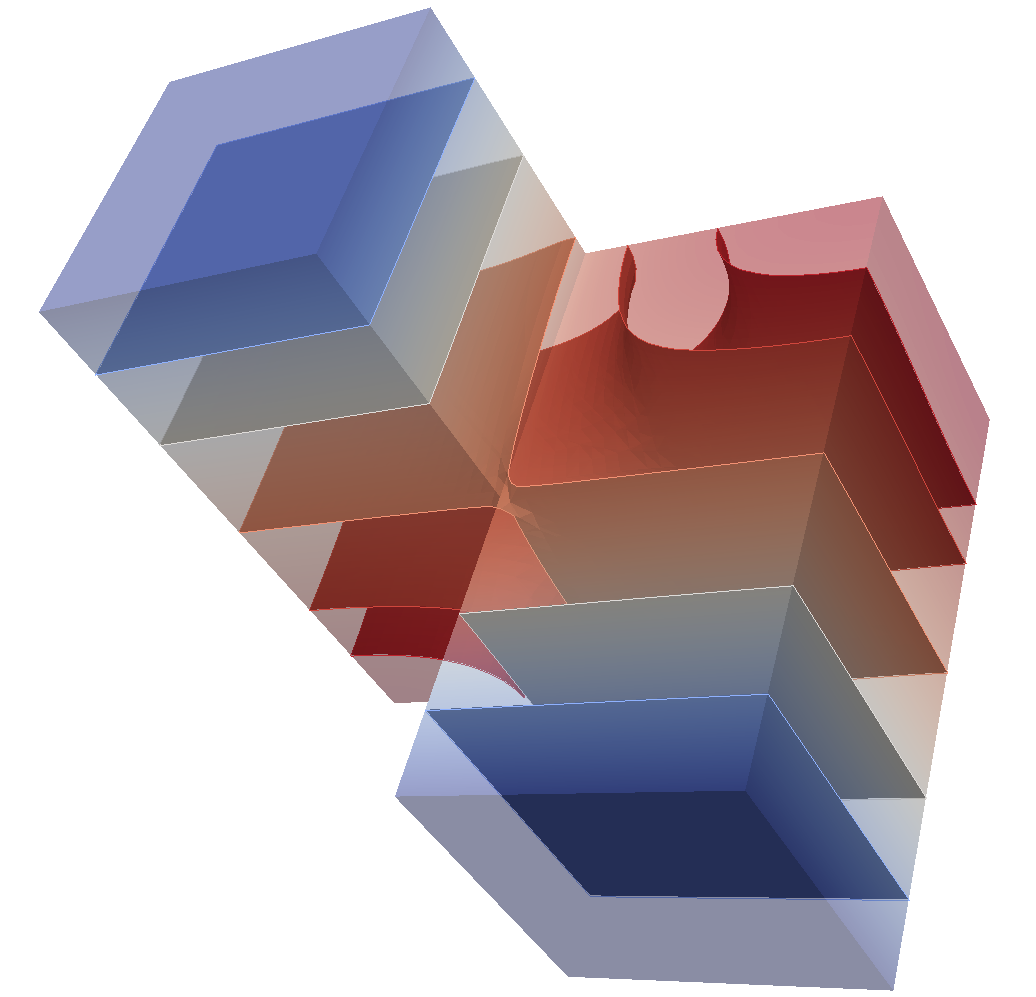
\includegraphics[width=100mm]{ModelPDE_Sol}
\caption{The field values of the structure as visualized with Paraview. Isosurfaces are 
defined for field values 0.5, 1.0, 1.5, 1.8 and 1.9, respectively.}\label{fg:post1}
\end{center}
\end{figure}


\subsection*{Further possibilities}

Here are some things you could try out, or are at least possible. The menus of the GUI are just 
elementary so more advanced features may need that the keywords are added by hand to the 
command file. No coding is needed to implement these features though. 
\begin{itemize}
\item You can also solve the problem with an unstructured tetrahedral mesh using Gmsh format file \texttt{winkel.msh}. 
\item Play with the reaction, diffusion, convection coefficient, and also the advection velocity.
As far as they remain constant the equation should be solvable with one sweep.
\item You could try to use Neumann or Robin BCs as well. Remember though that
a steady state equatios needs definitions that uniquely define the solution.
\item Make the problem time-dependent. Note that then you most likely need to define the 
coefficient for the time derivative. 
\item When the advection increases in size the solution may becore eventually oscillatory.
To eliminate that some bubbles or p-elements may be needed. You may play around with 
element settings, for exammple use \texttt{Element = p:2} or \texttt{Element = n:1 b:1} etc. 
\item You could try to increase the number of elements either by using \texttt{-relh} 
parameter in ElmerGUI, or setting \texttt{Mesh Levels = 2} in Simulation section.
\item You could try to use \texttt{MATC} to make the coefficients parameter dependent.
Dependence on the solution itself introduces nonlinearities that might not be well handled 
by the fixed point iteration scheme. For more demanding nonlinearities Newton linearization or
other technniques may be needed. 
\item Also some periodicity could be introduced to this problem by letting the 
two extreme surface patches have a dependence between them.
\item You could introduce sort of contact conditions for the surface or bulk values 
of the problem by defining minimum or maximum values for the field. 
\end{itemize}


\hfill
\mbox{}








\graphicspath{{./}{ElasticBeam3D/}}
\chapter{Linear elasticity equation -- Loaded elastic beam -- 3D}

\modinfo{Directory}{ElasticBeam3D}
\modinfo{Solvers}{\Idx{StressSolve}}
\modinfo{Tools}{\Idx{ElmerGUI}}
\modinfo{Dimensions}{3D, Steady-state}
\modinfo{Author}{Peter R{\aa}back}


\subsection*{Case definition}

Assume a homogenous, elastic beam being rigidly supported on one 
end. On the other end it is subjected with a load of 2000~N
resulting from an attached object in the gravitational field. The gravity affects also the beam itself.
The length of the beam is 1~m and the thickness is 0.05~m, and the width 
0.1~m.
Material properties of the beam are those of dry pine timber:
Poisson 
ratio 0.37, Young's modulus $10\cdot 10^9$N/m$^2$, and density 550~kg/m$^3$. 
The problem is to solve the displacement and stress field of the beam.  
Here the \texttt{StressSolve} routine based on the 
linear theory of elasticity is applied.


\subsection*{Solution procedure}

The mesh is given in ElmerGrid format in file \texttt{beam3d.grd}, load this file.
\ttbegin
File 
  Open -> beam3d.grd
\ttend
You should obtain your mesh and may check that it consists of 6073 nodes and of 
1200 quadratic hexahedral elements. The second order elements give
improved accuracy compared to the first order elements as they avoid the phenomenom known as locking.
\begin{figure}[h!]
\begin{center}
  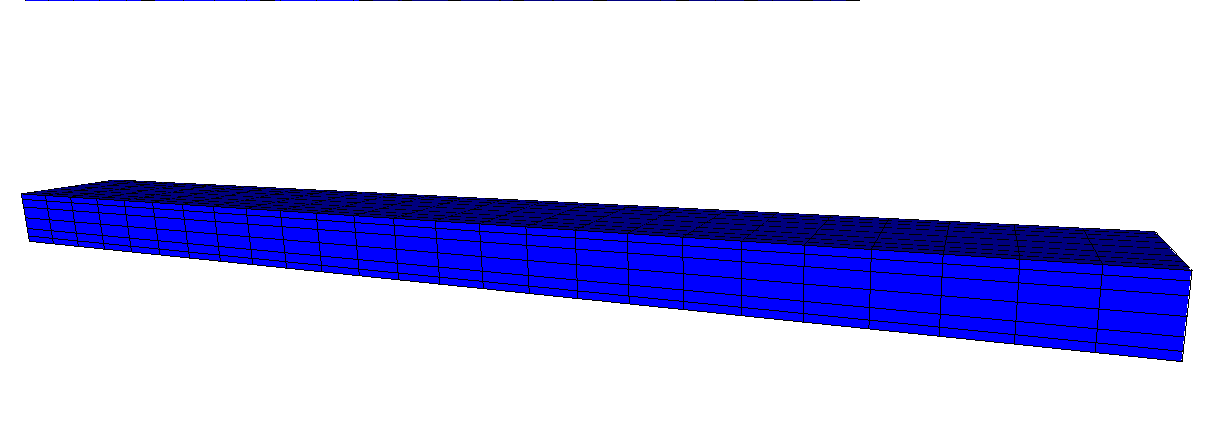
\includegraphics[width=0.8\textwidth,viewport=0 0 1230 300,clip]{beam_mesh}
  \caption{The mesh used in the computations}
  \label{fig:elast_mesh}
\end{center}
\end{figure}

After we have the mesh we start to go through the Model menu from the top to bottom. 
In the Setup we choose things related to the whole simulation such as file names, 
time stepping, constants etc.
The simulation is carried in steady-state in 3-dimensional Cartesian
coordinates. 
\ttbegin
Model
  Setup 
    Simulation Type = Steady state
    Steady state max. iter = 1
\ttend

In the Equation section we choose the relevant equations which in this case only includes 
the \texttt{Linear elasticity} equation
which solves the problem according to 
linear elastic theory. We also want to compute the stresses as a post-processing step.
For the linear system solvers we change the default settings in order
to obtain a better convergence in this case. As the equation is fully linear
we also eliminate the non-linear iteration loop. 
\ttbegin
Model
  Equation
    Name = Elasticity
    Apply to Bodies = Body 1
    Linear elasticity
      Active = on
      Calculate Stresses = on
    Edit Solver Setting
      Linear System
        Method = Iterative / GCR
        Preconditioning = ILU1
      Nonlinear system 
        Max. iterations = 1
      Apply
    Add 
    OK
\ttend        

The Material section includes all the material parameters.
They are divided into generic parameters which are direct properties of the material
without making any assumptions on the physical model, such as the mass. Other properties assume
a physical law, such as Young's modulus and Poisson ratio. 
\ttbegin
Model
  Material
    Name = Pine
    General 
      Density = 550 
    Linear Elasticity 
      Youngs Modulus = 10.0e9
      Poisson ratio = 0.37
    Apply to Bodies = Body 1 
    Add
    OK
\ttend

In this case there is a body force i.e. the gravity acting on the beam.
We assume that the gravity points to the negative $y$ direction.
\ttbegin
Model
  BodyForce
    Name = Gravity
    Linear Elasticity 
      Force 2 = $ -9.81 * 550
    Apply to Bodies = Body 1 
    Add
    OK
\ttend
Here we use a \texttt{MATC} expression for computing the volume force. This
expression is constant and is computed when the command file is interpreted.

Convergence should be obtained with the default 
initial condition i.e. zero for all fields, hence no initial condition is applied.

The first boundary condition fixes the beam rigidly at the wall.
The second boundary condition distributes the load of 2000~N uniformly on the 
area of 5.0e-3~m$^2$.
\ttbegin
Model
  BoundaryCondition
    Name = Wall
    Linear elasticity
      Displacement 1 = 0.0
      Displacement 2 = 0.0
      Displacement 3 = 0.0
    Add
    New

    Name = Mass
    Linear elasticity 
      Force 2 = -4.0e5
    Add 
\ttend   

The conditions may also be assigned to boundaries in the Boundary condition menu, or 
by clicking with the mouse. Here we use the latter approach as that spares us of the 
need to know the indexes of each boundary. 
\ttbegin
Model
  Set boundary properties
    Choose the wall end of the beam -> set boundary condition Wall
    Choose the other end of the beam -> set boundary condition Mass
\ttend

For the execution 
ElmerSolver needs the mesh files and the command file. We have now basically defined
all the information for ElmerGUI to write the command file. After writing it we may also visually 
inspect the command file.
\ttbegin
Sif 
  Generate
  Edit -> look how your command file came out  
\ttend

Before we can execute the solver we should save the files in a directory. The project includes
all the files needed to restart the case.
\ttbegin
File 
  Save Project
\ttend

After we have successfully saved the files we may start the solver
\ttbegin
Run
  Start solver
\ttend
The simulation may take a minute or so depending on the 
speed of the processor.
This time the convergence monitor does not have a meaningful output since 
of the different steps only one is related to the actual solution and the six other
ones to the computation of stresses with the Galerkin method.


\subsection*{Results}

When there are some results to view we may start the postprocessor, this time we use Paraview.
\ttbegin
Run
  Start Paraview
\ttend
Choose the \texttt{displacement} as the color field to plot.
The maximum displacement is $6.36$~cm 
You may also choose various stress components, or the von Mises stress.
Also you may choose to see \texttt{Surface With Edges} to visualize the mesh also. 
The resulting picture is shown in Fig~\ref{fig:beam_stresses}
\begin{figure}[h!]
\begin{center}
  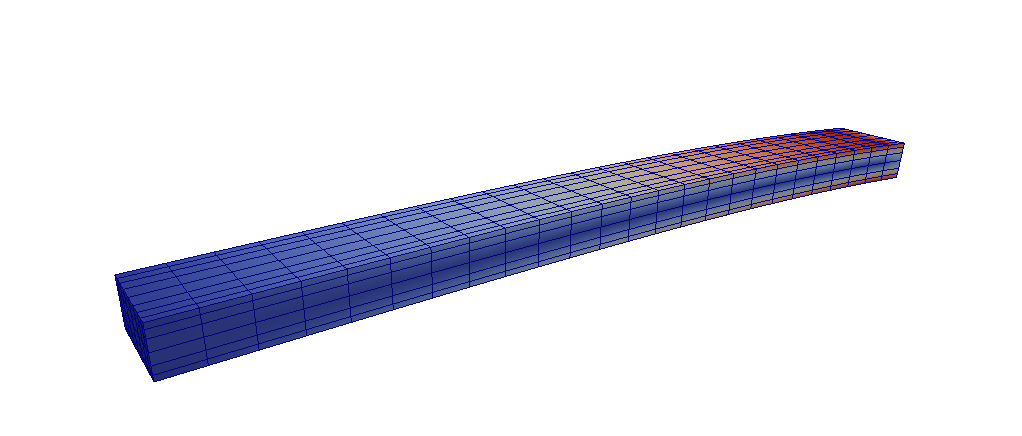
\includegraphics[width=0.8\textwidth]{beam_vonMises}
  \caption{The displaced shape of the elastic beam colored with the 
  von Mises stresses.}
  \label{fig:beam_stresses}
\end{center}
\end{figure}

Note that the displacements are so large that the assumption of linearity may be severely questioned.
When further increasing the loading one should resort to a solver that is able to catch the 
geometric non-linearities -- the ElasticSolver.


\subsection*{Extra task: Gravity in $x$ direction}

The beam should be more rigid if the beam is oriented differently.
For that aim, change the direction of gravity to orient in the negative $x$.
Change the body force
\ttbegin
Model
  BodyForce
    Linear Elasticity 
      Force 1 = $ -9.81*550
    Update
    OK
\ttend
and the boundary condition
\ttbegin
Model
  BoundaryCondition
    Linear elasticity 
      Force 1 = -4.0e5
    Update
    OK
\ttend   
The rigidity should scale as $dh^3$ and hence the maximum displacement should be reduced roughly 
to one quarter of the original.
 

\vfill
\mbox{}


\graphicspath{{./}{ElasticHookNonlinear/}}
\chapter{Non-linear elasticity equation --3D -- Loaded elastic curve}

\modinfo{Directory}{ElasticHookNonlinear}
\modinfo{Solvers}{\Idx{ElasticSolve}}
\modinfo{Tools}{\Idx{ElmerGUI}}
\modinfo{Dimensions}{3D, Transient}
\modinfo{Author}{Peter R{\aa}back}


\subsection*{Case definition}

An elastic U-shaped cylinder is pressed from its ends such that
the object faces large displacements. The material properties of
stainless steel are used. Problem is to gradually increase the displacement
and visualize the increase of stresses. The problem requires the use
of solver capable of dealing with large displacement.


\subsection*{Solution procedure}

The definitions for the relevant equation are not loaded into ElmerGUI by default. Hence, 
one needs to load these before starting the simulations.
\ttbegin
File 
  Definitions
    Append -> nonlinearelasticity.xml
\ttend
The additional definitions should reside in the directory \texttt{edf-extra} within the distribution.\\

The mesh is given in ElmerGrid format in file \texttt{u\_turn.grd},
load this file.
\ttbegin
File 
  Open -> u\_turn.grd
\ttend
You should obtain your mesh and may check that it consists of 12288 trilinear elements and 13585 nodes.
\begin{figure}[h!]
\begin{center}
  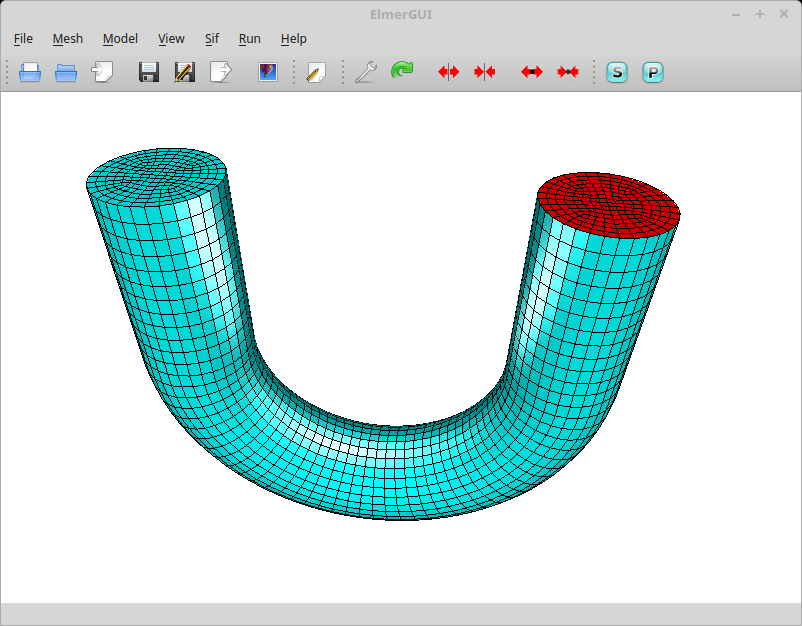
\includegraphics[width=0.6\textwidth]{UturnElmerGUI}
  \caption{The mesh used in the computations as shown in ElmerGUI.}
  \label{fig:UturnElmerGUI}
\end{center}
\end{figure}

After we have the mesh we start to go through the Model menu from the top to bottom. 
In the Setup we choose things related to the whole simulation such as file names, 
time stepping, constants etc.
The simulation is carried as a transient problem in 3-dimensional Cartesian
coordinates. The inertial forces of no importance so we could as well scan through a set of steady state
loading conditions. We choose the time step such that the total time being simulated is 1~s.
We assume that the original mesh (with diameter 0.6 is given units of cm. Hence we need to scale the
system down to work in SI units. 
\ttbegin
Model
  Setup 
    Simulation Type = Transient
    Timestep Sizes = 0.05
    Timestep Intervals = 20
    Coordinate Scaling = 0.01
\ttend

In the Equation section we choose the relevant equations which in this case only includes 
the \texttt{Nonlinear elasticity} equation.  We have just one body and therefore its easy to assign 
the Equation and Material to it directly.  We can use linear system solvers we are happy to 
use the defaults. One may however, try out different preconditioners (ILU1,\ldots) or more 
efficient iterative methods (BiCGStabl), for example.
\ttbegin
Model
  Equation
    Name = Elasticity
    Apply to Bodies = 1
    Nonlinear elasticity
      Active = on
      Edit Solver Settings
        Calculate Stresses = on
        Calculate Principal = on
    Add 
    OK
\ttend        
Here we choose the stainless steel from the material library.
You may click trough the material parameters of the various solvers to ensure that
the properties are indeed as they should be. Any consistent set of units may be used in Elmer.
The natural choice is of course to perform the computations in SI units. 
\ttbegin
Model
  Material
    Material library    
      Austenitic stainless steel (AK Steel 201)
    Apply to Bodies = 1 
    Add
    OK
\ttend

There are no body forces and convergence should be easily obtained with the default 
initial condition i.e. zero for all fields. Hence we don't need to toggle these subitems. 

We need to type now boundary conditions that we will later assign with the mouse to some surfaces.
We set boundary conditions for both ends of the hook such that
they close with respect to each other with time. The distance travelled in 1~s will be set to
0.006~m i.e. to same as the radius. The other displacement components are set to zero.  
To type in the multiline expressions for the boundary condition just press \texttt{Enter}
\texttt{Displacement 1} checkbox.
Note that the semicolon is an alternative separator
to line break. 
\ttbegin
Model
  BoundaryCondition
    Name = MovingRight
    Nonlinear elasticity
      Displacement 1 = Variable "time"
        Real MATC "0.006*tx"
      Displacement 2 = 0.0
      Displacement 3 = 0.0
    Add
    New

    Name = MovingLeft 
    Nonlinear elasticity
      Displacement 1 = Variable "time"
        Real MATC "-0.006*tx"
      Displacement 2 = 0.0
      Displacement 3 = 0.0
    Add 
\ttend   

The conditions may also be assigned to boundaries in the Boundary condition menu, or 
by clicking with the mouse. Here we use the latter approach as that spares us of the 
need to know the indexes of each boundary.
\ttbegin
Model
  Set boundary properties
    Choose negative x end -> set boundary condition "MovingRight"
    Choose positive x end  -> set boundary condition "MovingLeft"
\ttend

For the execution 
ElmerSolver needs the mesh files and the command file. We have now basically defined
all the information for ElmerGUI to write the command file. After writing it we may also visually 
inspect the command file.
\ttbegin
Sif 
  Generate
  Edit -> look how your command file came out  
\ttend

Before we can execute the solver we should save the files in a directory. The project includes
all the files needed to restart the case.
\ttbegin
File 
  Save Project
\ttend

After we have successfully saved the files we may start the solver
\ttbegin
Run
  Start solver
\ttend
A convergence view automatically pops up showing relative changes of each iteration.
As there are 20 time steps the convergence will be shown for each time step.
You can start looking at the results already after a few time steps. The whole simulation
takes a few minutes. 
\ttbegin
Run
  Start ParaView
\ttend


\begin{figure}[h!]
\begin{center}
  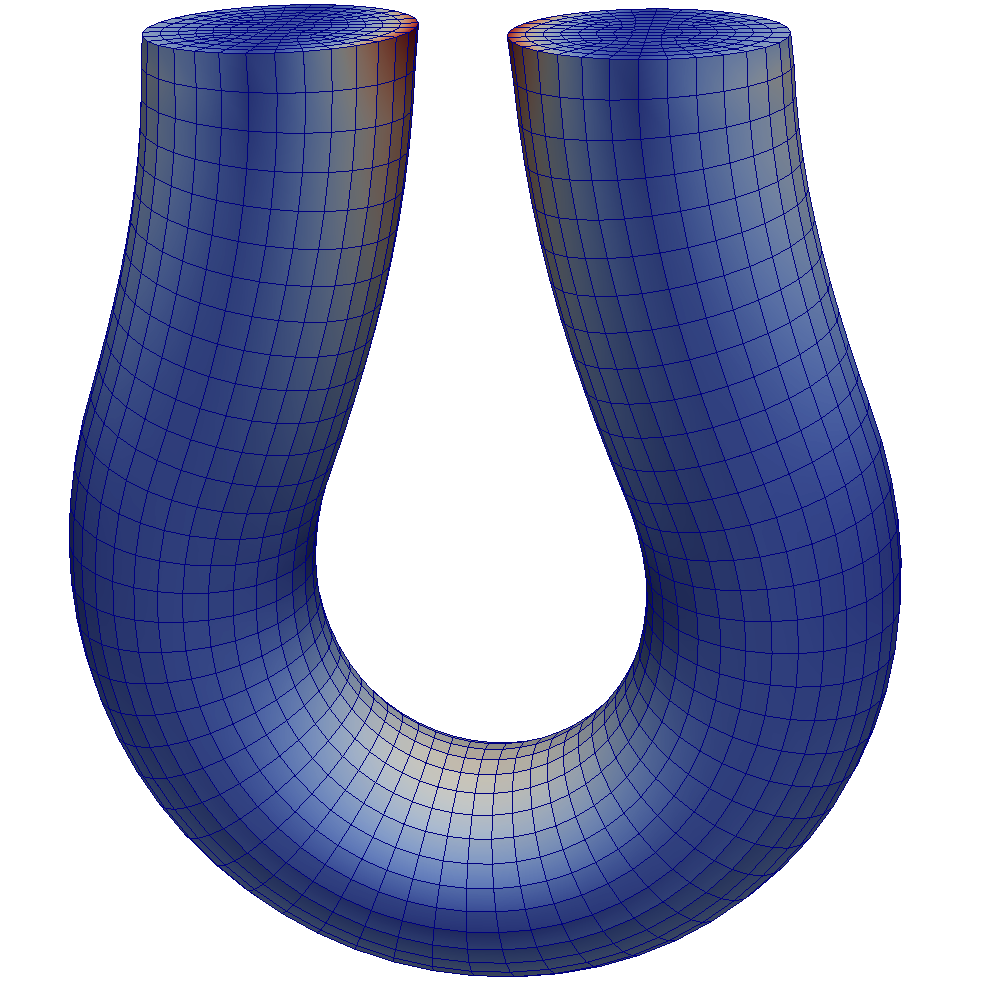
\includegraphics[width=0.5\textwidth]{UturnVonMisesStressMesh}
  \caption{The final state of the deformed curve. Color shows the resulting von Mises stresses.}
  \label{fig:UturnVonMisesStress}
\end{center}
\end{figure}

In reality the material could break at some point. Here we have assumed a linear material law
even though the geometric displacement makes the equation non-linear. 


\subsection*{Alternative task: Rotating square profile}

You may perform the tutorial with an alternative geometry: \texttt{square\_profile.grd}.
Follow almost the same logic except now we rotate the ends of the beam.

We need to enforce rigid body rotations to the ends of the mesh. The following
types of Dirichlet conditions need to be implemented
\begin{equation}
  \begin{array}{ll}
    u_x = & ( \cos(\phi) - 1)x - \sin(\phi)y ) \\
    u_y = & ( \cos(\phi) - 1)y + \sin(\phi)x )     
  \end{array}
\end{equation}
These can be set using the following \texttt{MATC} function
\ttbegin
  Displacement 1 = Variable "time, Coordinate"
    Real MATC "(cos(tx(0)*pi)-1.0)*tx(1)-sin(tx(0)*pi)*tx(2)
  Displacement 2 = Variable "time, Coordinate"
    Real MATC "(cos(tx(0)*pi)-1.0)*tx(2)+sin(tx(0)*pi)*tx(1)
\ttend 
Note that the argument to \texttt{MATC} is always called \texttt{tx} and it holds the
parameters in the given order. In this case component "0" refers to \texttt{time}, component "1" to
\texttt{Coordinate 1} (i.e. x), and component "2" to \texttt{Coordinate 2} (i.e. y). 
The multiplier for the trigonometric functions is $\pi$ which means that a revolation of
180 degrees is performed in 1 second. 
 
\begin{figure}[h!]
\begin{center}
  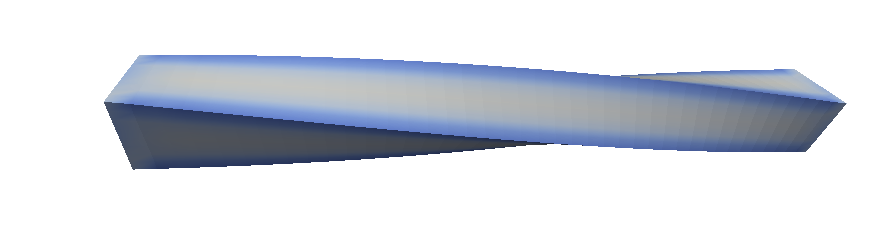
\includegraphics[width=0.6\textwidth]{RotatingProfile50}
  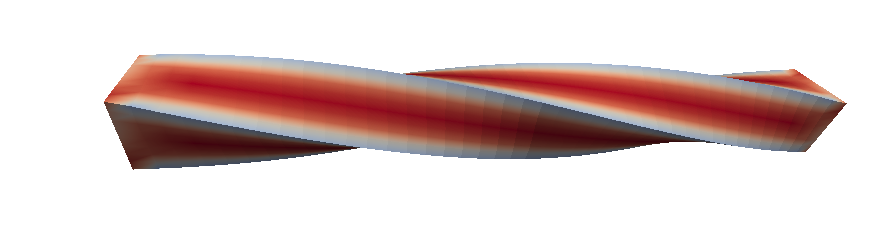
\includegraphics[width=0.6\textwidth]{RotatingProfile100}
  \caption{A square profile being rotated from one end by 90 and 180 degrees. Color shows the von Mises stresses.}
  \label{fig:RotatingProfile}
\end{center}
\end{figure}



\vfill
\mbox{}


\graphicspath{{./}{ElasticPlateEigenmodesGUI/}}
\chapter{Smitc solver -- 2D -- Eigenmodes of an elastic plate}

\modinfo{Directory}{ElasticPlateEigenmodesGUI}
\modinfo{Solvers}{\Idx{SmitcSolver}} 
\modinfo{Tools}{\Idx{ElmerGUI}} 
\modinfo{Dimensions}{2D, Eigenmode}
\modinfo{Author}{Peter R{\aa}back}


\subsection*{Problem description}

For thin elastic structures it is often advisable to use dimensionally reduced models i.e. 
study plates or shells. In this tutorial we compute the few lowest eigenmodes of an elastic plate. 
Our geometry is a simple pentagon which (compared to a square) eliminates some of the trivial symmetries.
The pentagon is rigidly fixed at all boundaries.

For more details on the solver we refer to the documentation of Smitc solver in the 
Elmer Models Manual.

\subsection*{Solution procedure}

Start \texttt{ElmerGUI} from command line or by clicking the icon in your desktop. Here we describe 
the essential steps in the ElmerGUI by writing out the clicking procedure. Tabulation generally means that the 
selections are done within the window chosen at the higher level. 

Before we can start the set-up we should make sure that the menus for Smitc solver are present.
If not, they may be found in file
\ttbegin
$ELMERHOME/bin/edf-extra/elasticplate.xml
\ttend
To load these definitions do the following
\ttbegin
File
  Definitions
    Append -> choose the file
\ttend
To see what kind of new menu structures were loaded you may play around with viewer collapsing and opening. 
Note that if you want to load an existing project you should load the xml-definitions that were used 
in creating the project. Therefore it may be best to place all actively used menu definitions in
directory
\ttbegin
$ELMERHOME/bin/edf
\ttend

When the menu structures for plate solver are there then we are ready to continue.
The mesh is given in 2d netgen format in file \texttt{pentagon.grd} in the samples directory of ElmerGUI, 
load this file.
\ttbegin
File 
  Open -> pentagon.in2d
\ttend
You should obtain a pentagon consisting of 5 triangles. To increase the number of elements 
change the parameters passed on to the nglib library by going to
\ttbegin
Mesh 
  Configure
    nglib / Max H: 0.05
\ttend
You may check in the \texttt{Model summary} 
window that it consists of 1199 nodes and 2276 linear triangles.
If the mesh was successfully imported your window should look something in figure~\ref{fg:pentagonmesh}.

\begin{figure}
\begin{center}
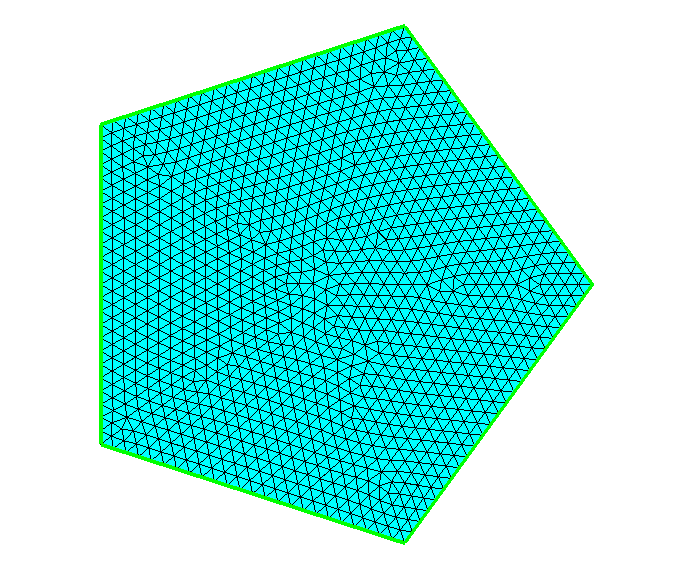
\includegraphics[width=100mm]{mesh}
\caption{The finite element mesh in ElmerGUI}\label{fg:pentagonmesh}
\end{center}
\end{figure}

After we have the mesh we start to go through the Model menu from the top to bottom. 
In the \texttt{Setup} we choose things related to the whole simulation such as file names, 
time stepping, constants etc.
The simulation is carried out in 2-dimensional Cartesian
coordinates and in steady-state (also used for eigenmodes). 
Only one steady-state iteration is needed as the case is linear. 
\ttbegin
Model
  Setup 
    Simulation Type = Steady state
    Steady state max. iter = 1
    Apply
\ttend

In the equation section we choose the relevant equations and parameters related to their solution. 
When defining Equations and Materials it is possible to assign to the bodies immediately, or to use mouse
selection to assign them later. In this case we have just one body and therefore its easier to assign 
the Equation and Material to it directly.

For the solver setting we need to activate the eigen mode computation. We also choose the 
direct umfpack solver which for small 2D problems often performs great.
\ttbegin
Model
  Equation
    Add 
      Name = Plate Equation
      Apply to bodies = 1
      Elastic Plates
        Active = on
        Edit Solver Settings 
          Solver Specific Options
            Eigen Analysis = on
            Eigen System Values = 10
          Linear System
            Direct = on
              Umfpack              
    Add  
    OK
\ttend        

The Material section includes all the material parameters.
They are divided into generic parameters which are direct properties of the material
without making any assumptions on the physical model, such as the mass. Other properties assume
a physical law, such heat Young's modulus. As our problem is academic in nature we choose some 
simple ideal parameters but data from material database could also be used instead.
\ttbegin
Model
  Material
    Add 
      Name = Ideal
      Apply to bodies = 1 
      General    
        Density = 1000.0
      Elastic Plates
        Youngs Modulus = 1e9
        Poisson ratio = 0.3
        Thickness = 0.001
        Tension = 0.0	
      Add
      OK
\ttend

A Body Force represents the right-hand-side of a equation i.e. external forces. In eigenmode analysis
no body forces are used. Nor are any Initial conditions required.

In this case all the boundaries are rigidly fixed we set all the components of the 
solution field to be zero. The 1st component is the displacement in the normal direction
while the 2nd and 3rd components are its derivatives in $x$ and $y$ directions.
\ttbegin
Model
  BoundaryCondition
    Add 
      Elastic Plates
        Deflection 1 = 0.0
        Deflection 2 = 0.0
        Deflection 3 = 0.0
      Name = Fixed
      Apply to boundaries = 1 2 3 4 5
      Add
      OK
\ttend   

For the execution 
ElmerSolver needs the mesh files and the command file. We have now basically defined
all the information for ElmerGUI to write the command file. After writing it we may also visually 
inspect the command file.
\ttbegin
Sif 
  Generate
  Edit -> look how your command file came out  
\ttend

Before we can execute the solver we should save the files in a directory. In saving the project all the
necessary files for restarting the case will be saved to the 
destination directory.
\ttbegin
File 
  Save Project
\ttend

After we have successfully saved the files we may start the solver
\ttbegin
Run
  Start solver
\ttend
A convergence view automatically pops up showing relative changes of each iteration.
In this case there is just one iteration and thus no curve appears.

\subsection*{Results}
The resulting eigenvalues are shown in table~\ref{tb:pentagonres}.
Note that some eigenmodes are degenerated but as the finite element mesh is not
perfectly symmetric there will be minor differences in the eigenvalues.

\begin{table}[h]
\caption{Ten lowest eigenvalues for the pentagon plate}
\label{tb:pentagonres}
\begin{center}
\begin{tabular}{ll} \hline
No & $\omega^2$ \\ \hline
1 & 18.9 \\
2,3 & 81.3 \\
4,5 & 214.5 \\
6   & 281.1 \\
7, 8 & 472.5 \\
9, 10 & 621.0 \\ \hline
\end{tabular}
\end{center}
\end{table}

Note: if you face problems in the solution phase and need to edit the setting, always remember to save
the project before execution.

To view the results we here start Paraview
\ttbegin
Run
  Paraview
\ttend
and select the 1st component of the \texttt{deflection} field
(confusingly named the x-component). 
If one chose for vtu output the mode \texttt{Eigen Analysis = True} then each file includes
one eigenmode. Then the eigenmodes may be treated as time steps. 
In figure~\ref{fg:pentagonpost} some of the lowest eigenmodes are depicted.
\begin{figure}
  \begin{center}
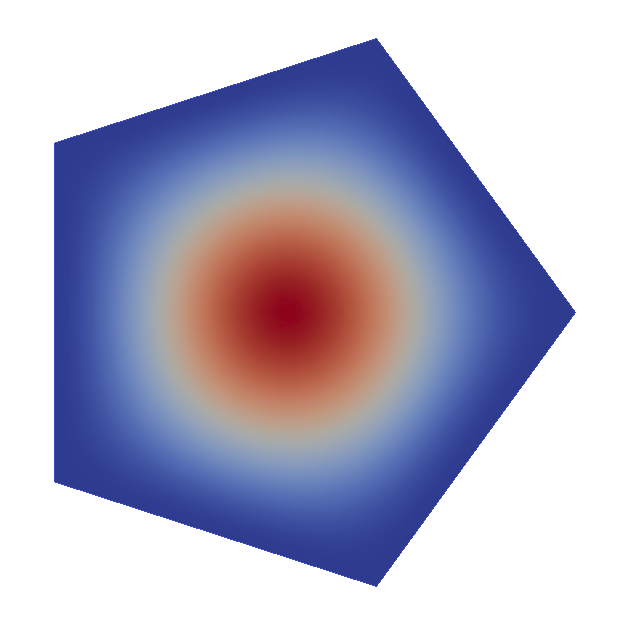
\includegraphics[width=40mm]{mode1}
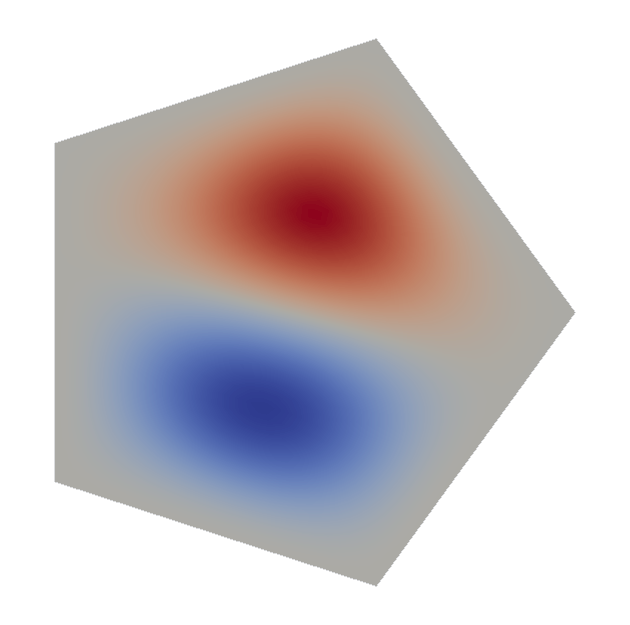
\includegraphics[width=40mm]{mode2}
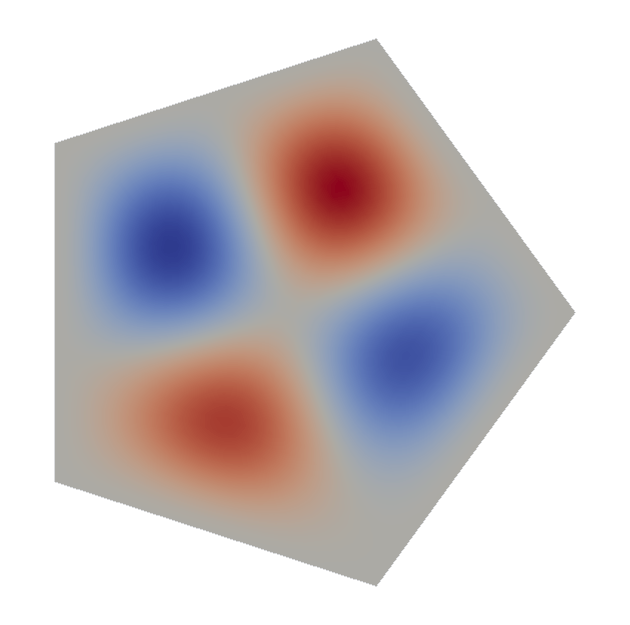
\includegraphics[width=40mm]{mode4} \\
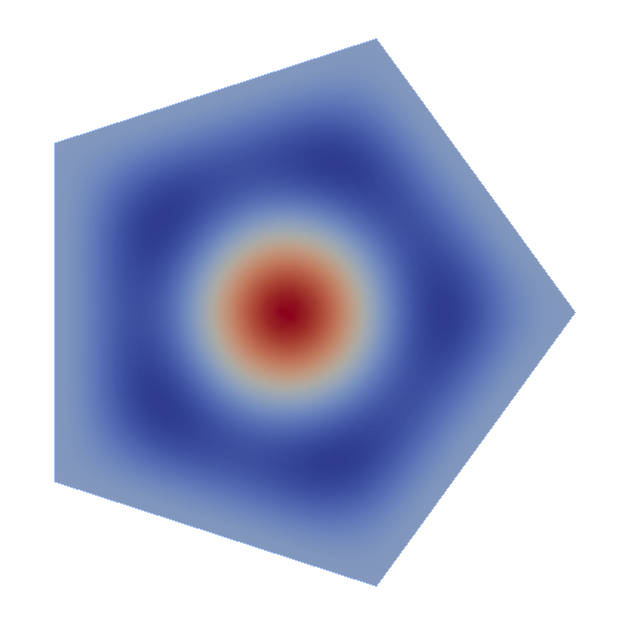
\includegraphics[width=40mm]{mode6}
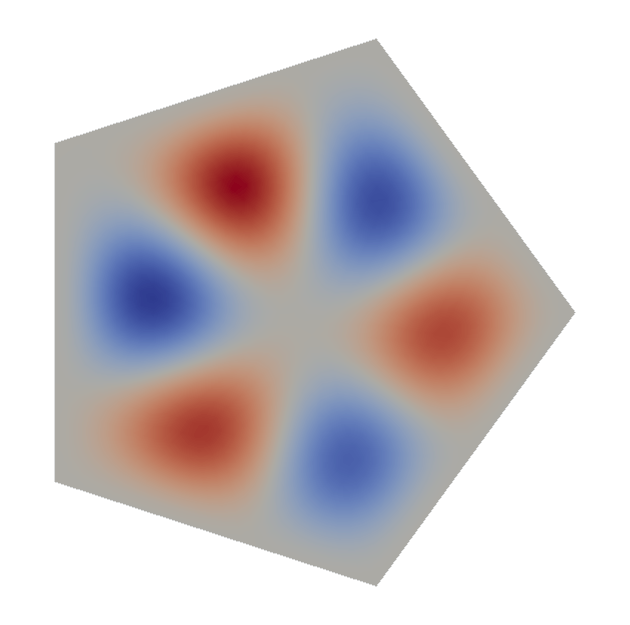
\includegraphics[width=40mm]{mode7}
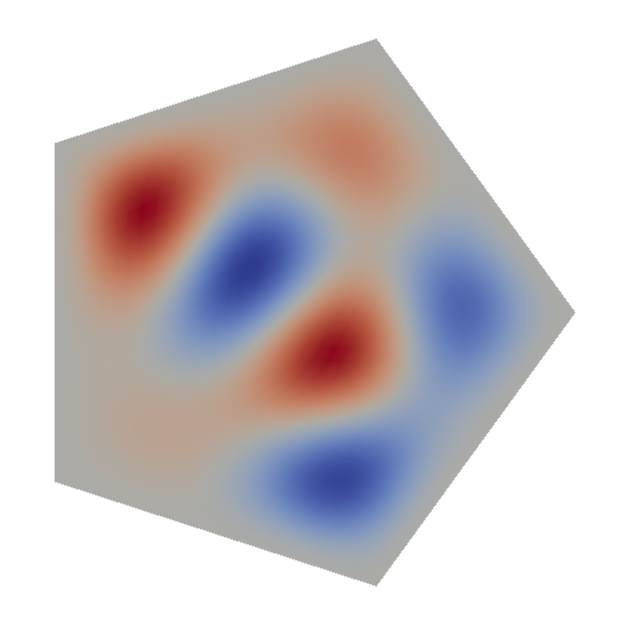
\includegraphics[width=40mm]{mode9}
\caption{The 1st, 2nd, 4th, 6th, 7th and 9th eigenmode of the plate. The displacement in the normal direction (first component) is shown.}
\label{fg:pentagonpost}
\end{center}
\end{figure}

\subsection*{Extra task}
You may test the effect of pre-stressing by altering the Tension material parameter.  

There are other similar geometries that you could use i.e. \texttt{hexagon.in2d}, \texttt{heptagon.in2d}, 
\texttt{octagon.in2d}.
When the number of vertices is increased the eigenvalues should slightly decrease. 



\hfill
\mbox{}








\graphicspath{{./}{CapacitanceOfTwoBalls/}}
\chapter{Electrostatic equation -- Capacitance of two balls}

\modinfo{Directory}{CapacitanceOfTwoBalls}
\modinfo{Solvers}{\Idx{StatElecSolver}}
\modinfo{Tools}{\Idx{netgen},\Idx{ElmerGUI}}
\modinfo{Dimensions}{3D, Steady-state}
\modinfo{Author}{Peter R{\aa}back}



\subsection*{Case definition}

This case presents the solution of the capacitance of perfectly conducting balls in free space. 
A voltage difference between the balls results to electric charge being introduced to the system. The balls have 
also self-capacitance that comes from the voltage difference with the far field. Therefore a symmetric capacitance matrix
with of size $2\times2$ needs to be solved.
The capacitances may be computed from two different voltage configurations.
For both the electrostatic equation is solved automatically. 

The problem does not have an analytical solution in a closed form. 
However, the cross-capacitance between the balls may be approximated from the series solution in \footnote{TUW-101191, PHD Dissertation by Christoph Wasshuber, About Single-Electron Devices and Circuits, {I}nstitut f{\"u}r {M}ikroelektronik, 1997, Appendix A.3, Capacitance of Two Spheres, \url{https://www.iue.tuwien.ac.at/phd/wasshuber/} }:
\begin{equation}
C_{12} = 4 \pi \varepsilon \frac{a^2}{d}\left ( 1 + \frac{a^2}{d^2-2a^2} + \frac{a^4}{d^4-4d^2a^2 + 3a^4}+ \ldots \right )
\end{equation}
and the self-capacitance from 
\begin{equation}
C_{10} = C_{20} = 4 \pi \varepsilon a \left ( 1 - \frac{a}{d} + \frac{a^2}{d^2-a^2} - \frac{a^3}{d^3-2da^2}+ \ldots \right )
\end{equation}
Let's mark $\tilde{C} = C / \varepsilon$. In this case $\tilde{C}_{12} \approx 1.191$ and $\tilde{C}_{10} \approx 5.019$.
Unfortunately the error bounds are not given.

In this particular case 
the balls are assumed to have a radius of $a=0.5$ and they are placed at distance $d=2$ apart from 
each other (measured from the ball origins). 


\subsection*{Meshing with Netgen (Optional)}

If you have Netgen installed and running, then you can generate the mesh before starting ElmerGUI, following the below instructions.  

If you don't have Netgen available, don't worry, an Elmer mesh has been provided in the `CapacitanceOfTwoBalls'  subfolder under `tutorials-GUI-files'.  Just load the ElmerGUI project in that subfolder, and it will load the mesh for you.  After loading the mesh, skip ahead to the next section, `Solution Procedure'.

If you have Netgen installed, then meshing is performed with the graphical user interface of Netgen. Netgen creates tetrahedral quality meshes and provides a native output for Elmer.
At the time of writing this tutorial the quadratic elements had some problems with numbering 
but these should not affect the linear elements.

The file is given as netgen geometry format in file \texttt{TwoBallsInBall.geo}. The geometry definition includes the 
two smaller balls inside a bigger ball. Ultimately the bigger ball would be infinitely large. As this is impossible 
here we choose a modest radius of 5. The larger this value, the better the far-field approximation of the 
electrostatic solution is.

The content of the file is given below:
\ttbegin
#
# a large ball with two smaller balls cut off
#
algebraic3d
solid smallballs = sphere (-1.0, 0.0, 0.0; 0.5)
           or sphere (1.0, 0.0, 0.0; 0.5);
solid bigball = sphere (0.0, 0.0, 0.0; 5.0);
solid rest = bigball and not smallballs;
tlo rest -col=[0,0,1] -transparent;
\ttend

Open the file and apply the default meshing. In this example two consecutive uniform refinements were performed 
(choose \texttt{Refine Uniform} under \texttt{Refinemenent}) so that the 
final mesh consisted of 41\,693 nodes and 238\,976 linear tetrahedrons. 

To save the mesh first choose under \texttt{File} the \texttt{Export Filetype} to be \texttt{Elmer}. Then choose
\texttt{Export Mesh} and save the mesh into a suitable directory to be opened
by ElmerGUI. 

\begin{figure}[h]
\centering
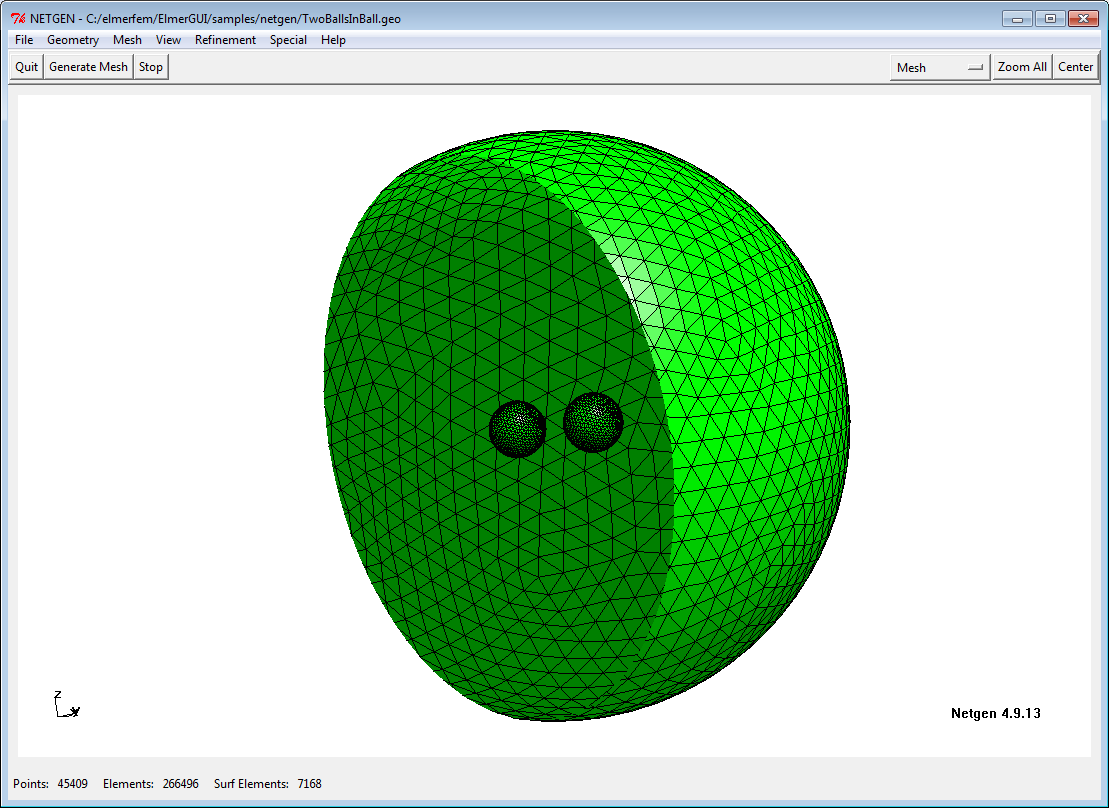
\includegraphics[width=140mm]{netgen_capture}
\caption{Surface mesh for the two inner balls as seen in Netgen}\label{fg:ballsnetgen}
\end{figure}  

The order of the mesh using nodal elements 
may be increased by \texttt{ElmerGrid}. Assuming the mesh would reside in directory \texttt{meshlin}
a mesh consisting of quadratic elements may be performed with the following command:
\ttbegin
ElmerGrid 2 2 meshlin -increase -out meshquad
\ttend
This will maintain the number of elements but the number of nodes will, in this case, increase to 359\,009. 


\subsection*{Solution procedure}

The definitions for the electrostatic equation may not have been loaded into ElmerGUI by default. If this is the case 
one needs to load these before starting the simulations.
\ttbegin
File 
  Definitions
    Append -> electrostatics.xml
\ttend
The additional definitions should reside in the directory \texttt{edf-extra} within the distribution.
Moving the desired \texttt{xml} files to the \texttt{edf}-directory enables automatic loading of the 
definitions at start-up. By inspecting the definitions in the \texttt{Elmer Definitions File editor} one
may inspect that the new definitions were really appended. 


The mesh is already created, load it from the directory that was created above.
\ttbegin
File 
  Load Mesh -> mesh
\ttend

\begin{figure}[h]
\centering
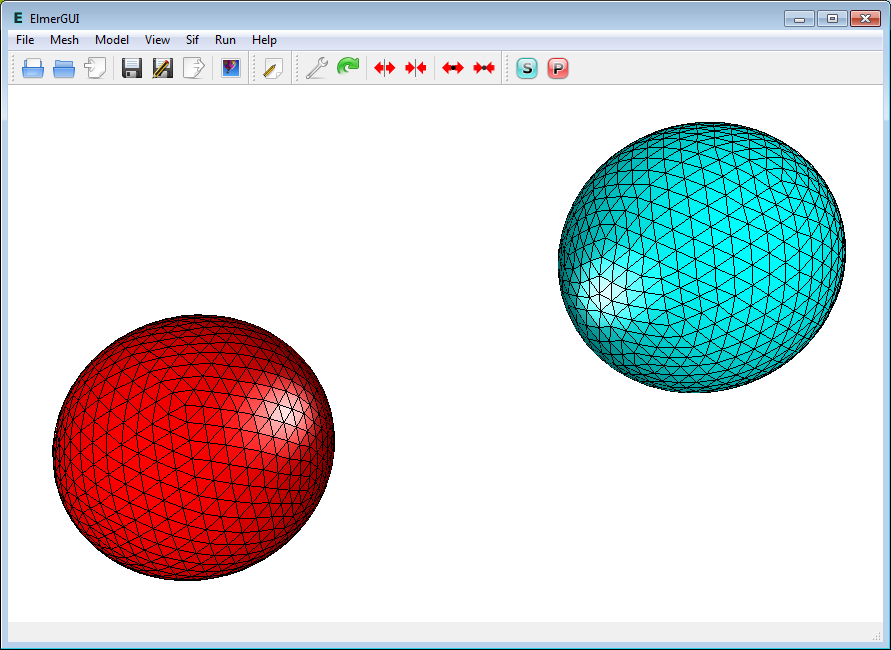
\includegraphics[width=140mm]{ElmerGUI_capture}
\caption{The mesh with one highlighted ball as seen in ElmerGUI}\label{fg:ballselmergui}
\end{figure}  

The display in ElmerGUI upon loading the mesh will show the outside of the large ball.  
To view the inner two smaller balls, double click on the outside of the large ball, then 
click on `Hide/show selected'.

\ttbegin
View 
  Hide/show selected   Ctrl+H
\ttend


After we have the mesh we start to go through the Model menu from the top to bottom. 
In the Setup we choose things related to the whole simulation such as file names, 
time stepping, constants etc.
The steady-state simulation is carried out in 3-dimensional Cartesian
coordinates. For convenience we also set the permittivity of vacuum $\varepsilon_0$ equal to one.
This makes it easier to compare the results to the analytical expressions. 
\ttbegin
Model
  Setup 
    Simulation Type = Steady state
    Vacuum Permittivity = 1.0
\ttend
In the equation section we choose the relevant equations and parameters related to their solution. 
In this case we'll have only the electrostatics solver. 

When defining Equations and Materials it is possible to assign to the bodies immediately, or to use mouse
selection to assign them later. In this case we have just one body and therefore its easier to assign 
the Equation and Material to it directly.

In the solver specific options we want to activate some flags that are needed to invoke the 
computation of derived fields. 
For the linear system solvers we are happy to use the defaults. One may however, try out different
preconditioners (ILU1,\ldots) or direct Umfpack solver, for example.
\ttbegin
Model
  Equation
    Name = Electrostatics
    Apply to Bodies = 1
    Electrostatics
      Active = on
      Edit Solver Settings
        Solver specific options
          Calculate Capacitance Matrix = True
          Calculate Electric Field = True
          Calculate Electric Energy = True
    Add 
    OK
\ttend        
The Material section includes all the material parameters.
In this case we only have the relative permittivity $\varepsilon_r$ which we set to one.
\ttbegin
Model
  Material
    Name = Ideal
    Electrostatics
      Relative Permittivity = 1.0
    Apply to Bodies = 1 2
    Add
    OK
\ttend

We have two boundary conditions for the potential at the ground and at the capacitor. For other boundaries
the do-nothing boundary results to zero flux over the boundary.
\ttbegin
Model
  BoundaryCondition
    Name = Farfield
    Electrostatics
      Electric Infinity BC = True
    Add
    New

    Name = CapBody1
    Electrostatics
      Capacitance Body = 1
    Add
    New

    Name = CapBody2
    Electrostatics
      Capacitance Body = 2
    Add
\ttend   

The conditions may also be assigned to boundaries in the Boundary condition menu, or 
by clicking with the mouse. Here we use the latter approach as that spares us of the 
need to know the indexes of each boundary.
\ttbegin
Model
  Set boundary properties
    Choose Outer sphere -> set boundary condition Farfield
    Choose one inner sphere -> set boundary condition CapBody1
    Choose the other inner sphere -> set boundary condition CapBody2
\ttend

For the execution 
ElmerSolver needs the mesh files and the command file. We have now basically defined
all the information for ElmerGUI to write the command file. After writing it we may also visually 
inspect the command file.
\ttbegin
Sif 
  Generate
  Edit -> look how your command file came out  
\ttend

Before we can execute the solver we should save the files in a directory. The project includes
all the files needed to restart the case.
\ttbegin
File 
  Save Project
\ttend

After we have successfully saved the files we may start the solver
\ttbegin
Run
  Start solver
\ttend
A convergence view automatically pops up showing relative changes of each iteration.
The equation is fully linear and hence only two iterations are needed -- the second 
one just ensures that convergence of the non-linear level was really obtained. 
The norm of the solution should be 0.36356324.

When the solution has finished we may start the postprocessor to view some results.
\ttbegin
Run
  Start ParaView
\ttend


\subsection*{Results}

The essential result of this case are the values of the capacitance matrix.
In this case $\tilde{C}_{12} \approx 1.691$ and $\tilde{C}_{10} \approx 5.019$.
For linear elements the obtained figures are 1.6983, 5.0793 and 5.0812, 
for quadratic Lagrange elements 1.6641, 5.0340 and 5.0340, respectively, and
finally for quadratic p-elements 1.6856, 4.9863 and 4.9884. 

The values are rather satisfactory with a difference less than 2\% from the series approximation.


\begin{figure}[h]
\centering
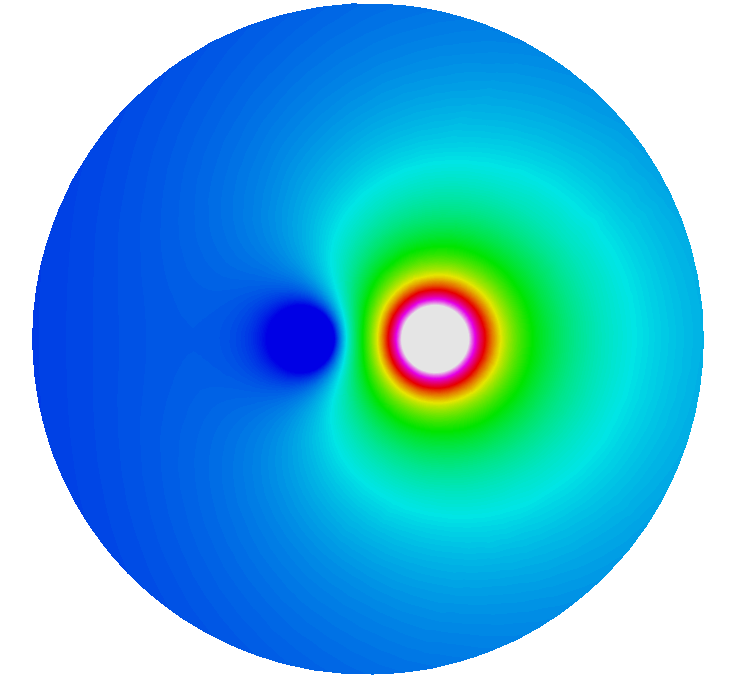
\includegraphics[width=120 mm]{ElmerPost_capture2}
\caption{The electrostatic potential on the clipping plane. This is the latter of the two symmetric configurations where the
unit voltage is applied to one ball and zero voltage to the other, respectively.}\label{fg:ballspost}
\end{figure}  

Note that the derived fields in the StatElecSolver are computed 
by averaging the fields over elements -- not using the 
Galerkin method which would provide optimal accuracy. To get optimal accuracy, use 
\texttt{FluxSolver}, for example.



\graphicspath{{./}{MagneticFieldWire/}}
\chapter{Magnetic field induced by harmonic current in a wire}

\modinfo{Files}{wire.grd}
\modinfo{Solvers}{\Idx{WhitneyAVHarmonicSolver}}
\modinfo{Tools}{\Idx{ElmerGrid}, \Idx{ElmerGUI}}
\modinfo{Dimensions}{3D, Harmonic}
\modinfo{Author}{Peter R{\aa}back}


\subsection*{Case definition}

This case demonstrates the simplest case on how to utilize the edge element based solvers
for computation of magnetic and electric fields.

Consider a simple copper wire with radius $R=0.01$~m. A potential difference of 1~V/m is applied
over the wire. We want to know the magnetic field strength around the wire.  

For steady state we have a simple analytical solution for reference.
\begin{equation}
\vec{A} = \left \{
\begin{array}{ll}
  -\frac{I\mu_0}{2\pi}\ln (r/R) \vec{e}_z, & \, \, \, r > R \\
  -\frac{I\mu_0}{4\pi R^2 } (r^2 - R^2) \vec{e}_z, & \, \, \, r \leq R 
\end{array}  
\right .
\end{equation}
resulting to a magnetic flux density
\begin{equation}
\vec{B} = \left \{
\begin{array}{ll}
  \frac{I\mu_0}{2\pi r}\vec{e}_\phi, & \, \, \, r > R \\
  \frac{I\mu_0}{2\pi R}\frac{r}{R}\vec{e}_\phi, & \, \, \, r \leq R 
\end{array}  
\right .
\end{equation}
We can solve the current from Ohms law to obtain the maximum field value at $r=R$ to be
\begin{equation}
  | \vec{B} | = \frac{1}{2} \mu_0 R \sigma | \vec{E} |   
\end{equation}
Using elecric conductivity of copper ($\sigma$=59.59e6 A/m$^2$V) we obtain 0.0374~T.

We are interested in what happens when the voltage is applied sinusoidally with a frequency of 100~kHz.
The harmonic case is unfortunately much more difficult to solve and no simple analytical expression exists.
Therefore we need to solve the problem numerically. 


\subsection*{Solution procedure}

The definitions for the relevant equation are not loaded into ElmerGUI by default. Hence, 
one needs to load these before starting the simulations.
\ttbegin
File 
  Definitions
    Append -> magnetodynamics.xml
\ttend
The additional definitions should reside in the directory \texttt{edf-extra} within the distribution.
Moving the desired \texttt{xml} files to the \texttt{edf}-directory enables automatic loading of the 
definitions at start-up. By inspecting the definitions in the \texttt{Elmer Definitions File editor} one
may inspect that the new definitions were really appended. 

The mesh is already defined in ElmerGrid format as file \texttt{wire.grd}. Load it from the \texttt{samples} directory were it resides.
\ttbegin
File 
  Open -> wire.grd
\ttend
The ElmerGrid plug-in of ElmerGUI will read the mesh and create the mesh for ElmerGUI using the ElmerGrid plug-in.
Note that the user
could also create the mesh directly on the command line by
\ttbegin
ElmerGrid 1 2 wire.grd
\ttend
and then use the \texttt{Load Mesh} option in \texttt{ElmerGUI} to take the mesh into use. 
If the user wants to modify the default mesh that can be done by editing the file directly.
The mesh has been constructed so that it can capture some boundary layer phenomena that we expect to take
place on the surface of the wire. In principle the mesh could be even shorter since the results do not really
depend on the axial direction. 


\begin{figure}[h]
\centering
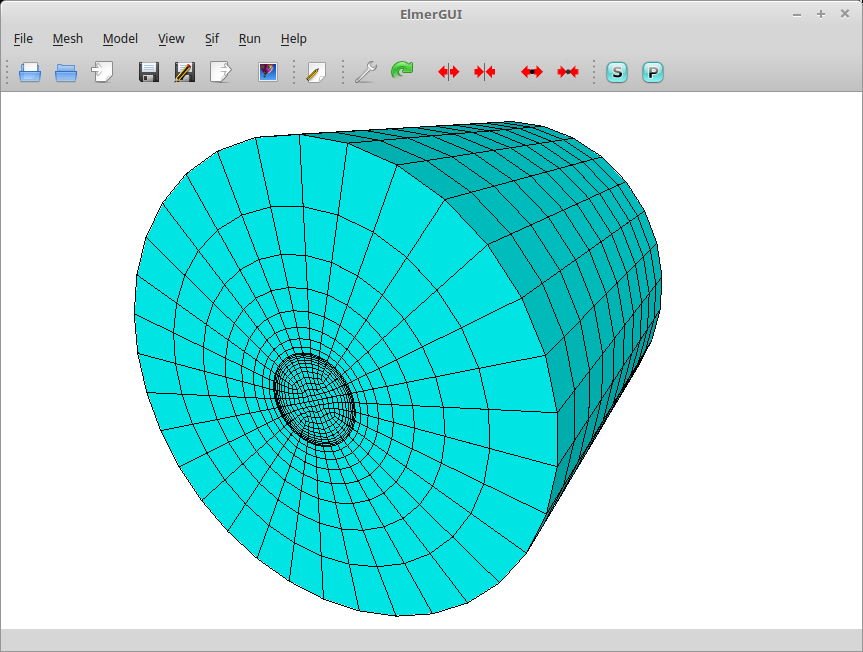
\includegraphics[width=140mm]{WireElmerGUI}
\caption{The mesh for the wire and surrounding air as seen in ElmerGUI}\label{fg:WireElmerGUI}
\end{figure}  


After we have the mesh we start to go through the Model menu from the top to bottom. 
In the Setup we choose things related to the whole simulation such as file names, 
time stepping, constants etc.
The steady-state simulation is carried out in 3-dimensional Cartesian
coordinates. The initial size of the mesh is 1000 times too large. Hence we apply scaling in this menu.
Also we want to use an harmonic equation that requires the frequency to be set somewhere. 
\ttbegin
SetUp
  Coordinate Scaling 
    1.0e-3
  Angular Frequency
    1.0e5   
\ttend
Currently the permeability of vacuum is not given
in the ElmerGUI. To set other than the default value for it (in case using a different unit system),
the free text box can be used.

In the equation section we choose the relevant equations and parameters related to their solution. 
In this case we'll have the \texttt{MgDynHarm} solver (there exists also a steady-state/transient version of the solver
as \texttt{MgDyn}), as well as the postprocessing solver \texttt{MgDynPost}.

When defining Equations and Materials it is possible to assign to the bodies immediately, or to use mouse
selection to assign them later. In this case we know that body 1 is the wire and body 2 is the surrounding air and we
can apply the definitions directly.
They will have the same set of solvers but different material properties. 

The solver specific options may need some alternations. We choose a more suitable
linear solver strategy for the AV equation. 

For the postprocessing we add some fields to be computed and skip the computation of nodal fields since the
elemental fields are often preferable for discontinuous fields. 
We also want to ensure that the postprocessing solver is run just before saving the results, after the primary solver has been computed.

In the following the correct equation are chosen and the suitable solver specific options are chosen:
\ttbegin
Model
  Equation
    Name = MgDynHarm
      Active = on
      Apply to Bodies = 1 2  
      Edit Solver Settings
        Linear System
          Iterative = BiCGStabL
        Preconditioning = none
        BiCGStabl order = 4    
    Name = MgDynPost
      Active = on
      Edit Solver Settings
        Solver Specific Options
          Calculate Magnetic Field Strenth = on
          Calculate Joule Heating = on
          Skip Nodal Field = on
          Discontinuous Bodies = on
        General
          Execute Solver = before saving   
    Add 
    OK
\ttend        
The Material section includes all the material parameters. In this case we basically have two 
different materials -- the copper wire and the surrounding air.
We use the definitions from the small material database that comes with the code.
\ttbegin
Model
  Material
    Material Library
      Copper
    Apply to Bodies = 1
    Add
    New

  Material
    Material Library
      Air (room temperature)
    Apply to Bodies = 2
    Add
    OK
\ttend

We need to set the boundary conditions both for the scalar potential associated to the nodal degrees of freedom, \texttt{av},
and to the vector potential associated to the edge degrees of freedom, \texttt{av \{e\}}.
Both of these have both real and imaginary components. 
We set the scalar potential only for the conductors and the vector potential for all external boundaries.
\ttbegin
Model
  BoundaryCondition
    Name = Ground 
    MgDynHarm
      AV re = 0
      AV re {e} 1 = 0
      AV re {e} 2 = 0
      AV im = 0
      AV im {e} 1 = 0
      AV im {e} 2 = 0
    Add
    OK
\ttend   
For the other of the wire we have exactly the same BCs except that the scalar potential is set to 0.01~V to give the desired
electric field as the length of the wire is 0.01~m. 
\ttbegin
Model
  BoundaryCondition
    Name = Voltage
    MgDynHarm
      AV re = 0.01
      AV re {e} 1 = 0
      AV re {e} 2 = 0
      AV im = 0
      AV im {e} 1 = 0
      AV im {e} 2 = 0
    Add
    OK
\ttend   
and finally for all other extenal BCs we set the boundary non-axial components of the vector potential to zero.
\ttbegin
Model
  BoundaryCondition
    Name = AxialField
    MgDynHarm
      AV re {e} 1 = 0
      AV re {e} 2 = 0
      AV im {e} 1 = 0
      AV im {e} 2 = 0
    Add
    OK
\ttend 


The conditions may also be assigned to boundaries in the Boundary condition menu, or 
by clicking with the mouse. Here we use the latter approach as that spares us of the 
need to know the indexes of each boundary.
\ttbegin
Model
  Set boundary properties
    Choose one end of the wire -> set boundary condition to Ground
    Choose the other end of the wire -> set boundary condition to Voltage
    Choose all other external BCs -> set boundary condition to AxialField
\ttend

For the execution 
ElmerSolver needs the mesh files and the command file. We have now basically defined
all the information for ElmerGUI to write the command file. After writing it we may also visually 
inspect the command file.
\ttbegin
Sif 
  Generate
  Edit -> look how your command file came out  
\ttend

Before we can execute the solver we should save the files in a directory. The project includes
all the files needed to restart the case.
\ttbegin
File 
  Save Project
\ttend

After we have successfully saved the files we may start the solver
\ttbegin
Run
  Start solver
\ttend
A convergence view automatically pops up showing relative changes of each iteration.
The equation is fully linear and hence only two iterations are needed -- the second 
one just ensures that convergence of the non-linear level was really obtained. 
The convergence monitor also plots the postprocessing steps but they do not really converge as each field is computed just once. 

When the solution has finished we may start the postprocessor to view some results.
\ttbegin
Run
  Start ParaView
\ttend


\subsection*{Results}

Here we present some results of the computations. The visualization is done using Paraview and the \texttt{vtu} format.
For optimal visualization use the \texttt{Discontinuous Bodies} flag turned on both on the calculation of the fields
and while saving the results in \texttt{vtu} format. 
These flags ensure that the solution is enforces continuous over the
bodies while maintaining jumps between bodies. 
No other formats in Elmer can currently support these features.

\begin{figure}[h]
\centering
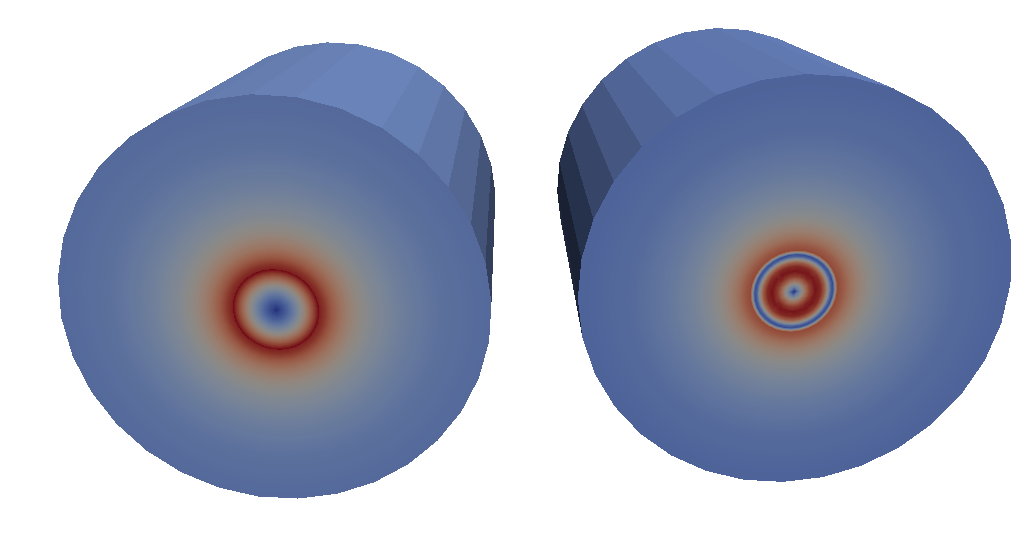
\includegraphics[width=120 mm]{WireBfieldReIm}
\caption{Imaginary and real parts of the magnetic field strength.}\label{fg:BfieldWire}
\end{figure}  

\begin{figure}[h]
\centering
\includegraphics[width=120 mm]{WireBfieldImVectors}
\caption{Imaginary part of the magnetic field strength plotted with vectors scaled by the field values.}
\label{fg:BfieldWireVectors}
\end{figure}  


The resulting absolute values of the imaginary and real part of the magnetic flux density are depicted in
Figure~\ref{fg:BfieldWire}. The imaginary part dominates in the amplitude the (0.524~T vs. 0.107~T). 
The corresponding vector field of the magnetic flux density is depicted in Figure~\ref{fg:BfieldWireVectors}.

Why are the results so far from the steady state solution? If you run the case again with 
100~Hz you can see that the solution is very close to the static one. The maximum magnetic flux density from the
computations is 0.0367~T which is very close to the analytical solution of 0.0374~T. So the frequency
really has an significant effect on the results!

You may study what happens when you increase the frequency further. At some point the mesh cannot capture the solution
properly any more and the results become questionable.


\hfill

\bibliography{tutorialsbib}
\bibliographystyle{plain}


\graphicspath{{./}{HorseShoeGUI/}}
\chapter{Magnetostatics -- Magnetic field resulting from a permanent magnet}

\modinfo{Directory}{Horseshoe}
\modinfo{Solvers}{\Idx{MagnetoDynamics2D}}
\modinfo{Tools}{\Idx{Gmsh}, \Idx{ElmerGUI}}
\modinfo{Dimensions}{2D, Steady-state}
\modinfo{Author}{Peter R{\aa}back}



\subsection*{Case definition}

This case roughly reproduces the case of a permanent magnet as demonstrated in 
the following link: \\
\url{http://www.strek.strefa.pl/students/meslec/lab06.pdf}

Consider a horseshoe-shaped permanent magnet. It consists of a ferromagnetic material but the two end 
sections are premagnetized in opposite directions. This results to a familiar magnetic field pattern.
The horseshoe consists of three different regions and additionally there is the surrounding air.
There is a circular outer boundary in order to conveniently allow for farfield conditions.  
The material is assumed to have a constant relative permeability of 5000 and the magnetization is 
set to 750~kA/m. 

Note that as this is a 2D case the resulting fields actually are those of an infinitely long 
horseshoe which of course does not make much sense in real life. 


\subsection*{Meshing}

The computational mesh is predefined in Gmsh format in file \texttt{horseshoe.msh}. 
If the user wants to modify the default mesh that must be done with Gmsh. The geometry of 
the file is given in file \texttt{horseshoe.geo}.


\subsection*{Solution procedure}

The definitions for the relevant equation are not loaded into ElmerGUI by default. Hence, 
one needs to load these before starting the simulations.
\ttbegin
File 
  Definitions
    Append -> magnetodynamics2d.xml
\ttend
The additional definitions should recide in the directory \texttt{edf-extra} within the distribution.
Moving the desired \texttt{xml} files to the \texttt{edf}-directory enables automatic loading of the 
definitions at start-up. By inspecting the definitions in the \texttt{Elmer Definitions File editor} one
may inspect that the new definitions were really appended. 

The mesh is already defined, load it from the \texttt{samples} directory were it recides.
\ttbegin
File 
  Open -> horseshoe.msh
\ttend
The ElmerGrid plug-in of ElmerGUI will read the mesh and convert it to a format understood by Elmer. 

\begin{figure}[h]
\centering
\includegraphics[width=140mm]{HorseShoeMesh}
\caption{The mesh for the horseshoe and surrounding air as see in ElmerGUI}\label{fg:horseshoeselmergui}
\end{figure}  


After we have the mesh we start to go through the Model menu from the top to bottom. 
In the Setup we choose things related to the whole simulation such as file names, 
time stepping, constants etc.
The steady-state simulation is carried out in 2-dimensional cartesian
coordinates. Nothing needs to be changed here. Currently the permeability of vacuum is not given
in the ElmerGUI. To set other than the default value for it, the free text box can be used. 

In the equation section we choose the relevant equations and parameters related to their solution. 
In this case we'll have the MgDyn2D solver, as well as the postprocessing solver MgDyn2DPost.

When defining Equations and Materials it is possible to assign the to bodies immediately, or to use mouse
selection to assign them later. In this case the equations need to be solved in all the bodies and 
hence clicking the all from 1 to 4 here is most convenient. We give a higher priority to the actual solver
so that the vector potential will be computed before the derived fields. 
In this case solver specific options should be ok but they could also be changed in this context.
\ttbegin
Model
  Equation
    Name = MgDyn2D
      Active = on
      Priority = 1
      Apply to Bodies = 1 2 3 4 
    Name = MgDyn2DPost
      Active = on
    Add 
    OK
\ttend        
The Material section includes all the material parameters. In this case we basically have two 
different materials but the differenyt magnetization must also be given as a material property.
Hence we actually need to define four materials.  
\ttbegin
Model
  Material
    Name = Air
    MgDyn2d
      Relative Permeability = 1.0
    Add
    New

    Name = Iron
    MgDyn2d
      Relative Permeability = 5000.0
    Add
    New

    Name = IronPlus
    MgDyn2d
      Relative Permeability = 5000.0
      Magnetization 1 = Real 750.0e3
    Add
    New

    Name = IronMinus
    MgDyn2d
      Relative Permeability = 5000.0
      Magnetization 1 = Real -750.0e3
    Add
    OK
\ttend

We may now assign the material properties by selecting with the mouse.
This spares us of the 
need to know the indexes of each body.
\ttbegin
Model
  Set body properties
    Choose air -> set Materail to Air
    Choose curved part of horseshoe -> set Material to Iron
    Choose upper straight part of horseshoe -> set Material to IronPlus
    Choose lower straight part of horseshoe -> set Material to IronMinus
\ttend

We have just one boundary condition i.e. the outer boundary for which we use the farfield condition.
\ttbegin
Model
  BoundaryCondition
    Name = Farfield
    MgDyn2D
      Infinity BC = True
    Add
    OK
\ttend   

The conditions may also be assigned to boundaries in the Boundary condition menu, or 
by clicking with the mouse. Here we use the latter approach as that spares us of the 
need to know the indexes of each boundary.
\ttbegin
Model
  Set boundary properties
    Choose the 4 pieces of the outer sphere -> set boundary condition Farfield
\ttend

For the execution 
ElmerSolver needs the mesh files and the command file. We have now basically defined
all the information for ElmerGUI to write the command file. After writing it we may also visually 
inspect the command file.
\ttbegin
Sif 
  Generate
  Edit -> look how your command file came out  
\ttend

Before we can execute the solver we should save the files in a directory. The project includes
all the files needed to restart the case.
\ttbegin
File 
  Save Project
\ttend

After we have successfully saved the files we may start the solver
\ttbegin
Run
  Start solver
\ttend
A convergence view automatically pops up showing relative changes of each iteration.
The equation is fully linear and hence only two iterations are needed -- the second 
one just ensures that convergence of the nonlinear level was really obtained. 
The norm of the solution should be 0.3679.

When the solution has finished we may start the postprocessor to view some results.
\ttbegin
Run
  Start ParaView
\ttend


\subsection*{Results}


\begin{figure}[h]
\centering
\includegraphics[width=120 mm]{HorseShoeA}
\caption{The vector potential of the magnetic field.}\label{fg:HorseShoeA}
\end{figure}  

\begin{figure}[h]
\centering
\includegraphics[width=120 mm]{HorseShoeB}
\caption{A closeup of the vector potential combined with the magnetic field intensity vectors. 
Note that the fields in the horseshoe itself have been
masked away to demonstrate the well known field shape in the free space.}\label{fg:HorseShoeB}
\end{figure}  


The resulting z-component of the vector potential is depicted in Figure~\ref{fg:HorseShoeA}.
The corresponding postprocessed magnetic field intensity is depicted in Figure~\ref{fg:HorseShoeB}. 
Note that the derived fields is enforced to be continuous by default which is not 
optimal for visualization. For optimal results use Discontinous Galerkin (DG) method
for the postprocessing. Note that when using DG the postprocessing should be done with .vtu files and 
Paraview. The postprocessing tools of Elmer cannot deal with elementwise-fields. 


\hfill

\bibliography{tutorialsbib}
\bibliographystyle{plain}


\graphicspath{{./}{FlowStepGUI/}}
\chapter{Navier-Stokes equation -- Laminar incompressible flow passing a step}
\label{tut:stepflowgui}

\modinfo{Directory}{FlowStepGUI}
\modinfo{Solvers}{\Idx{FlowSolve}}
\modinfo{Tools}{\Idx{ElmerGUI}}
\modinfo{Dimensions}{2D, Steady-state}
\modinfo{Author}{Peter R{\aa}back}


\subsection*{Case definition}

This tutorial represents the canonical step flow of viscous fluid. 
A fluid, flowing past a step (see figure~\ref{fg:struct2}), has the density
1~kg/m$�$ and viscosity 0.01~kg/ms. The velocity profile at the inlet is
parabolic with a mean velocity $<v_x>=1.0$~m/s and $v_y=0.0$~m/s. At the outlet only 
the vertical component is defined, $v_y=0.0$~m/s. At all other
walls the no-slip boundary condition, $\vec{v}=0$, is applied. 
Thus the Reynolds number for the case is around 100. 

\begin{figure}[h]
\centering
\includegraphics[width=100mm,viewport=0 30 800 270,clip]{geom}
\caption{Geometry of the step flow problem}\label{fg:struct2}
\end{figure}
%
Mathematically the problem to be solved is
\begin{equation}
\left \{
\begin{array}{rccl}
- \nabla \cdot (2 \mu \overline{\overline{\varepsilon}}) + \rho 
\vec{u} \cdot \nabla \vec{u} + \nabla p & = & 0 & \mbox{ in } \Omega \\
\nabla \cdot \vec{u} & = & 0 & \mbox{ in } \Omega \\
\end{array}
\right .
\end{equation}
%
with the boundary conditions
\begin{equation}
\left \{
\begin{array}{rccl}
u_x & = & 1 & \mbox{ on } \Gamma_{inlet} \\
u_x & = & 0 & \mbox{ on } \Gamma_{no-slip} \\
u_y & = & 0 & \mbox{ on } \Gamma_{inlet} \cup \Gamma_{outlet} \cup \Gamma_{no-slip} 
\end{array}
\right .
\end{equation}
where $\mu$ is the viscosity, $\overline{\overline{\varepsilon}}$ is 
the strain tensor,  $\rho$ is the density, $\vec{u}$ is the velocity and
$p$ is the pressure. It is assumed that the density and viscosity are 
constants. 



\subsection*{Solution procedure}

The mesh is given in ElmerGrid format in file \texttt{step.grd}, load this file.
\ttbegin
File 
  Open -> step.grd
\ttend
You should obtain your mesh and may check that it consists of 9696 nodes and of 
9442 bilinear elements.
\ttbegin
Model 
  Summary...
\ttend

After we have the mesh we start to go through the Model menu from the top to bottom. 
In the Setup we choose things related to the whole simulation.
The steady-state simulation is carried out in 2-dimensional Cartesian
coordinates, which are also the defaults.  
\ttbegin
Model
  Setup 
    Simulation Type = Steady state
    Coordinate system = Cartesian
\ttend
In the equation section we choose the relevant equations and parameters related to their solution. 
In this case the only the Navier-Stokes equation is needed.

When defining Equations and Materials it is possible to assign to the bodies immediately, or to use mouse
selection to assign them later. In this case we have just one body and therefore its easier to assign 
the Equation and Material to it directly. One could also edit the solver setting in order to
try different strategies for solving the non-linear or linear system. Initially the Navier-Stokes
solver uses the more robust Picard iteration which is changed to Newton iteration after few initial steps.
For the given viscosity the default values are ok, but may need tuning when going into higher Reynolds numbers.
\ttbegin
Model
  Equation
    Name = Navier-Stokes
    Apply to Bodies = Body 1
    Navier-Stokes 
      Active = on
      Edit Solver Setting
        Nonlinear System
          Max. iterations = 20
          Newton after iterations = 3
    Add 
    OK
\ttend        

The Material section includes all the material parameters.
They are divided into generic parameters which are direct properties of the material
without making any assumptions on the physical model, such as the density. Other properties assume
a physical law, such as viscosity. 
\ttbegin
Model
  Material
    Name = Ideal
    General 
      Density = 1.0
    Navier-Stokes 
      Viscosity = 0.01
    Apply to Bodies = Body 1 
    Add
    OK
\ttend

The current case does not have any body forces. Convergence should also be
obtained using the default initial condition which sets all field values to zero. 
Hence no setting for initial condition are needed. 

Only one boundary condition may be applied to each boundary and therefore all the 
different physical BCs for a boundary should be grouped together. In this case the
Temperature and Velocity. The side walls are assumed to be adiabatic.

The parabolic inlet-profile is achieved using the 
MATC environment. To be able to edit the content of the inlet profile 
click \texttt{Enter} to open an edit box for the \texttt{Velocity 1}. The given expression will be 
interpreted at run-time so that $v_x=6(y-1)(2-y)$. As $y\in[1,2]$ thereby
creating a parabolic velocity profile with a mean velocity of unity. 
\ttbegin
Model
  BoundaryCondition
    Name = Inlet
    Navier-Stokes 
      Velocity 1 = Variable Coordinate 2; Real MATC "6*(tx-1)*(2-tx)"
      Velocity 2 = 0.0
    Add
    New

    Name = Outlet
    Navier-Stokes 
      Velocity 2 = 0.0
    Add 
    New
 
    Name = Walls
    Navier-Stokes 
      Noslip wall BC = on
    Add
    OK
\ttend   

The conditions may also be assigned to boundaries in the Boundary condition menu, or 
by clicking with the mouse. Here we use the latter approach as that spares us of the 
need to know the indexes of each boundary.
\ttbegin
Model
  Set boundary properties
    Choose Inlet -> set boundary condition Inlet
    Choose Outlet -> set boundary condition Outlet
    Choose Walls -> set boundary condition Walls
\ttend

For the execution 
ElmerSolver needs the mesh files and the command file. We have now basically defined
all the information for ElmerGUI to write the command file. After writing it we may also visually 
inspect the command file.
\ttbegin
Sif 
  Generate
  Edit -> look how your command file came out  
\ttend

Before we can execute the solver we should save the files in a directory. The project includes
all the files needed to restart the case. Create a suitable directory for the case if needed. 
\ttbegin
File 
  Save Project
\ttend

After we have successfully saved the files we may start the solver
\ttbegin
Run
  Start solver
\ttend
A convergence view automatically pops up showing relative changes of each iteration.
The problem should converge in about ten iterations to a norm of 0.4347 visible on the output.

When there are some results to view we may start the postprocessor also
\ttbegin
Run
  Start ParaView
\ttend


\subsection*{Results}

The results may be viewed using the postprocessor as shown in Figure~\ref{fg:step_velo} and~\ref{fg:step_pres}. 
One may also register specific values,
for example the pressure difference is 0.388~Pa, the minimum and maximum lateral velocities
are -0.1666~m/s and 1.5~m/s, respectively.
One special result of interest 
is the point, on the x-axis, at which the direction of the flow changes. 
In this case its position is about 5.0~m after the step. 

\begin{figure}[h]
\centering
\includegraphics[width=15cm, viewport=0 30 900 270,clip]{velo_abs}
\caption{Absolute value of the velocity field}\label{fg:step_velo}
\end{figure} 

\begin{figure}[h]
\centering
\includegraphics[width=15cm, viewport=0 30 900 270,clip]{pres}
\caption{Pressure field}\label{fg:step_pres}
\end{figure} 

   




\subsection*{Extra task: Decreasing the viscosity}

Try what happens if the viscosity is further decreased by a factor 10. 
Convergence may be difficult to obtain. Some tricks that may be tested include
\begin{itemize}
\item Introducing a relaxation factor (typically in the range 0.5--0.7)
\item Increasing number of non-linear iterations
\item Favoring Picard iteration over Newton 
\item Increasing mesh density (and length of domain)
\end{itemize}
Don't be worried if you fail to find convergence. This task will mainly act as a 
motivator in using turbulence models for higher Reynolds numbers.

Remember to re-perform the following phases in order to get the updated results
\ttbegin
Sif 
  Generate
File 
  Save Project
Run
  Start solver
\ttend
You may just reload the results in the postprocessor rather than closing and opening the program.


\hfill


\graphicspath{{./}{VonKarmanGUI/}}
\chapter{Vortex shedding -- von Karman instability}

\modinfo{Directory}{VonKarmanGUI}
\modinfo{Solvers}{\Idx{FlowSolve}}
\modinfo{Tools}{\Idx{ElmerGUI}}
\modinfo{Dimensions}{2D, Transient}
\modinfo{Author}{Peter R{\aa}back}

\subsection*{Case definition}

%\begin{flushleft}
This tutorial is about simulating the development of vortex shedding i.e. the von Karman instability. 
The geometry is a tube with a circular obstacle. 
For more details on the problem look at the benchmark case definition by
by M. Sch�fer and S. Turek in \textit{"Benchmark computations of laminar flow around a cylinder"}.


\subsection*{Solution procedure}

The mesh is given in 2d netgen format in file \texttt{circle\_in\_channel.in2d}, load this file.
\ttbegin
File 
  Open -> circle_in_channel.in2d
\ttend
You should get a mesh consisting of 749 nodes and 1328 triangles. This
is a rather sparse mesh. To increase the element number 
\ttbegin
Mesh 
 Configure
   nglib / Max H: 0.02
Mesh 
  Remesh
\ttend
This mesh includes 3464 nodes and 6506 triangles. The mesh is presented in figure~\ref{fg:vonkarman_mesh}.

\begin{figure}[h]
\centering
\includegraphics[width=150 mm, height=55 mm]{vonkarman_mesh}
\caption{Computational mesh of the problem.}\label{fg:vonkarman_mesh}
\end{figure}  


After we have the mesh we start to go through the Model menu from the top to bottom. 
In the Setup we choose things related to the whole simulation such as file names, 
time stepping, constants etc.
The simulation is carried out in 2-dimensional Cartesian
coordinates. 2nd order bdf time stepping method is selected with 200 steps
and we want the total simulation time to be 8 seconds. 
\ttbegin
Model
  Setup 
    Simulation Type = Transient
    Steady state max. iter = 1
    Time Stepping Method = bdf
    BDF Order = 2
    Time Step Intervals = 200
    Time Step Sizes = $ 8/200
\ttend
For the solver specific settings we are quite happy to use the defaults. However, we relax a little bit the 
convergence tolerances to get speedier simulation.
\ttbegin
Model
  Equation
    Name = Navier-Stokes
    Apply to Bodies = 1
    Navier-Stokes 
      Active = on
    Edit Solver Settings
      Nonlinear system 
        Convergence tol. = 1.0e-4
      Linear System 
        Convergence tol. = 1.0e-6
    Add 
    OK
\ttend        
The Material section includes all the material parameters.
Here we choose simple parameters for the academic test case
\ttbegin
Model
  Material
    Name = Ideal
    General 
      Density = 1
    Navier Stokes
      Viscosity = 0.001 
    Apply to Bodies = 1 
    Add
    OK
\ttend

The system does not need any body forces. We are also happy with the default initial condition 
of zero and therefore no initial conditions are applied either. Any other initial condition would
require the values to be explicitly set.

We have three different kinds of boundaries: inlet, no-slip walls, and outlet. The inlet
has a parabolic fully developed laminar profile with a maximum velocity of 1.5~m/s.
Additionally for the inlet the vertical velocity component is assumed zero. 
The circle and the lower and upper walls are given the no-slip treatment.
For the outlet only the vertical component is set to zero since the default discretization
weakly imposes a zero pressure condition if the normal velocity component is not defined.
\ttbegin
Model
  BoundaryCondition
    Name = Inlet
    Navier-Stokes 
      Velocity 1 = Variable Coordinate 2; Real MATC "4*1.5*tx*(0.41-tx)/0.41^2"
      Velocity 2 = 0.0
    Add
    New

    Name = Walls
    Navier-Stokes 
      Velocity 1 = 0.0
      Velocity 2 = 0.0
    Add
    New

    Name = Outlet
    Navier-Stokes 
      Velocity 2 = 0.0
    Add 
    Ok
\ttend   

The conditions may also be assigned to boundaries in the Boundary condition menu, or 
by clicking with the mouse. Here we use the latter approach as that spares us of the 
need to know the indexes of each boundary.
\ttbegin
Model
  Set boundary properties
    Choose inlet -> set boundary condition Inlet
    Choose both horizontal walls and circle -> set boundary condition Walls
    Choose outlet -> set boundary condition Outlet
\ttend


For the execution 
ElmerSolver needs the mesh files and the command file. We have now basically defined
all the information for ElmerGUI to write the command file. After writing it we may also visually 
inspect the command file.
\ttbegin
Sif 
  Generate
  Edit -> look how your command file came out  
\ttend

Before we can execute the solver we should save the files in a directory. The project includes
all the files needed to restart the case.
\ttbegin
File 
  Save Project
\ttend

After we have successfully saved the files we may start the solver
\ttbegin
Run
  Start solver
\ttend
A convergence view automatically pops up showing relative changes of each iteration.
The norm after the first time step should be around 0.695, and after last 0.749, respectively.

When there are some results to view we may start the postprocessor also
\ttbegin
Run
  Start ParaView
\ttend


\subsection*{Results}

Due to the number of the time steps the simulation will take a few minutes.
You may inspect the results with Paraview as the time-steps are computed, or
wait until all time steps have been computed.
You need to reload the files if number of time steps are increased.

In Figure \ref{fg:vonkarman_flow} the velocity field is presented for three different time steps.
The maximum velocity in the system should be about 2.1724~m/s. Note that here
visualization was not performed with Paraview and may therefore look quite different.

\begin{figure}[h]
\centering
\includegraphics[width=12cm, viewport=0 30 1089 270,clip]{flow20.png}
\includegraphics[width=12cm, viewport=0 30 1089 270,clip]{flow100.png}
\includegraphics[width=12cm, viewport=0 30 1089 270,clip]{flow200.png}
\caption{Velocity distribution at steps 20, 100 and 200}\label{fg:vonkarman_flow}
\end{figure} 


\subsection*{Effect of Reynolds number}
The Reynolds number in this case is around 100 resulting to unsteady flow.
The critical Reynolds number is around 90 and 
reducing the flow velocity so that Reynolds number becomes, say 20, makes the 
system to possess a steady-state solution. On the other hand, increasing the velocity will make the von Karman vortices
even more pronounced until they break into fully chaotic motion. This finite element mesh will allow only 
a minor increase in Reynolds number to be able to capture the phenomena. 

\hfill



\graphicspath{{./}{CurvedPipeGUI/}}
\chapter{Thermal flow in curved pipe}

\modinfo{Directory}{CurvedPipeGUI}
\modinfo{Solvers}{\Idx{HeatSolve}, \Idx{FlowSolve}}
\modinfo{Tools}{\Idx{ElmerGUI}}
\modinfo{Dimensions}{3D, Steady-state}
\modinfo{Author}{Thomas Zwinger, Peter R{\aa}back}


\subsection*{Case definition}
 
%\begin{flushleft}

This tutorial demonstrates how to set up a coupled case
of thermal flow in curved pipe with a finite thickness. Within the pipe 
both the flow and heat transfer equations need to be solved while on the
solid section only heat transfer needs to be considered. 

The inner diameter of the pipe is 0.01~m and the outer ~0.012~m, respectively. 
It is bent to a 135 degree angle with a radius of 0.02~m. Beyond the bend
0.03~m of the direct part is also accounted for. 
The fluid flowing in the pipe is water with an original temperature of 350~K. 
The outer temperature of the iron pipe is 300~K making the water
gradually to cool. 

The water is injected with a parabolic velocity profile with a maximum
of 0.01~m/s. In reality the laminar analytic profile is described by the 
Bessel's function. Here the flow is treated as laminar and steady-state 
even though at these Reynolds number (about 100) the unsteady nature of the 
flow should probably be considered. This would enhance the heat transfer.
The steady-state case, however, will achieve the educational goals of the tutorial.

\subsection*{Solution procedure}

The mesh is defined in ElmerGrid format in file \texttt{curved\_pipe.grd}, load this file.
\ttbegin
File 
  Open -> curved\_pipe.grd
\ttend
You should obtain your mesh and may check that it consists of 23670 trilinear 
bricks and 25245 nodes. The density of the mesh may be varied by altering
the \texttt{Reference Density} in the file. For further information on
the mesh definition look at the \texttt{ElmerGrid} manual. Often it is 
desirable to use some professional mesh generation tool in CFD and 
translate it into Elmer format. For educational purposes we are 
quite happy to use this simple geometry.  

\begin{figure}[h]
\centering
\includegraphics[width=10cm]{curved_pipe_gui}
\caption{The mesh of the curved pipe as seen in ElmerGUI}\label{fg:curved_pipe_mesh}
\end{figure} 


After we have the mesh we start to go through the \texttt{Model} menu from the top to bottom. 
In the \texttt{Setup} we choose things related to the whole simulation such as file names, 
time stepping, constants etc.
The simulation is carried out in 3-dimensional Cartesian
coordinates in steady-state. There is nothing really to be done here, but you may verify that
the defaults are correct. 
\ttbegin
Model
  Setup 
    Coordinate system = Cartesian
    Simulation type = Steady state
    Steady state max. iter = 1
    ...
\ttend

In the Equation section we choose the relevant equations and parameters related to their solution. 
In this case we'll have two different sets of solvers (called as Equation in Elmer slang). 
The other consists of heat and flow solvers, while the 
other includes just the heat solver. We'll name them appropriately. 

When defining Equations and Materials it is possible to assign to the bodies immediately, or to use mouse
selection to assign them later. In this case we know that the fluid body has the index 1 and the 
solid body has the index 2. Therefore it is easy to assign the Equation and Material to the bodies directly. 

Here we neglect the effect of natural convection. Therefore there is just one-directional coupling from the 
flow to heat transfer. In order to follow the direction of causality we address the flow solver with a higher 
priority than the heat solver (default is zero). 	

Here we are quite happy with the default solver settings of the individual equations. 
However, for the flow solver we change the default preconditioner \texttt{ILU0} to \texttt{ILU1} to 
enhance convergence (with increased memory consumption). For 3D cases the direct solvers are usually 
not feasible so it is better to stick with the iterative \texttt{BiCGstab} linear solver. 
\\
The equation for the fluid
\ttbegin
Model
  Equation
    Add
    Name = Heat and Flow
    Apply to Bodies = 1
    Heat Equation
      Active = on
      Convection = Computed
    Navier-Stokes 
      Active = on
      Priority = 1
      Edit Solver Setting
        Linear System
          Preconditioning = ILU1
    OK
\ttend        
and then for the solid
\ttbegin
Model
  Equation
    Add
    Name = Just Heat
    Apply to Bodies = 2
    Heat Equation
      Active = on
      Convection = None
    OK
\ttend    


The Material section includes all the material parameters.
They are divided into generic parameters which are direct properties of the material
without making any assumptions on the physical model, such as the density. Other properties assume
a physical law, such as conductivities and viscosity. 

Here we choose water and iron from the material library.
You may click trough the material parameters of the various solvers to ensure that
the properties are indeed as they should be. Any consistent set of units may be used in Elmer.
The natural choice is of course to perform the computations in SI units. 

\ttbegin
Model
  Material
    Add
    Material library    
      Water (room temperature)
    Apply to Bodies = 1 
    OK

    Add
    Material library    
      Iron (generic)
    Apply to Bodies = 2
    OK
\ttend

The \texttt{Body force} section usually represents the right-hand-side of an equation. It could be used to account for the 
natural convection, for example. In this case, however, we do not apply any body forces.

Also an \texttt{Initial condition} could be given in steady-state case to enhance convergence. However, 
in this case convergence is pretty robust with the default guess of zero.

We have four different boundary conditions: thermal inflow, internal no-slip, 
outflow, and external fixed temperature. Otherwise natural BCs are assumed.
As it is tedious to know the indexes by heart we 
first define the different BCs and only afterwards apply them to the existing boundaries 
with the mouse. 

\ttbegin
Model
  BoundaryCondition
    Name = HotInflow
    Heat Equation
      Temperature = 350.0
    Navier-Stokes 
      Velocity 1 = 0.0
      Velocity 2 = 0.0
      Velocity 3 = Variable Coordinate 
        Real MATC "100.0*(1.0e-4-tx(0)^2-tx(1)^2)"
    Add
    New
\ttend
The condition for \texttt{Velocity 3} above may easiest be typed by pressing \texttt{Enter}-key in the
edit box which will open a larger window for editing.
\ttbegin
    Name = Outflow
    Navier-Stokes 
      Use normal-tangential coordinate system = on
      Velocity 2 = 0.0
      Velocity 3 = 0.0
    Add
    New

    Name = NoSlip
    Navier-Stokes 
      NoSlip Wall BC = on
    Add 
    New
 
    Name = Troom
    Heat Equation
      Temperature = 300.0
    Add
\ttend   

When choosing the boundaries it is important that you choose the right inlet.
For that purpose you may activate the compass, 
\ttbegin
View
  Compass = on
\ttend
Now the inlet is the one with normal pointing at the $z$-direction.
Now we are ready to choose the boundaries 
\ttbegin
Model
  Set boundary properties
    Choose inlet face -> set boundary condition HotInflow
    Choose outlet face -> set boundary condition Outflow
    Choose outer side -> set boundary condition Troom
\ttend
Unfortunately we cannot see the internal boundary. For that purpose click on the 
outer boundary and choose 
\ttbegin
View
  Hide/show selected
\ttend
The outer boundary should vanish and you can
proceed with the last BC,
\ttbegin
Model
  Set boundary properties
    Choose internal side -> set boundary condition Noslip
\ttend


For the execution 
ElmerSolver needs the mesh files and the command file. We have now basically defined
all the information for ElmerGUI to write the command file. After writing it we may also visually 
inspect the command file.
\ttbegin
Sif 
  Generate
  Edit -> look how your command file came out  
\ttend

Before we can execute the solver we should save the files in a directory. The project includes
all the files needed to restart the case. It's a good idea to give the project an illuminating name.
Avoid paths which includes empty spaces since they may cause problems later on. 
\ttbegin
File 
  Save Project
    Make New Folder -> curved_pipe
    OK
\ttend

After we have successfully saved the files we may start the solver
\ttbegin
Run
  Start solver
\ttend
A convergence view automatically pops up showing relative changes of each iteration.
The simulation may take a few minutes depending on your platform. 
After the simulation has terminated we may study the results.
\begin{figure}[h]
\centering
\includegraphics[width=10cm]{curved_pipe_convergence}
\caption{Convergence history of the case}\label{fg:curved_pipe_convergence}
\end{figure} 

\subsection*{Results}

The computed norms should be 3.255 for the Navier-Stokes equation and
324.66 for the heat equation. If there is some discrepancy the setup of the system
was probably different from the one in the tutorial.

After the simulation has terminated we may open the postprocessor to view the results.
\ttbegin
Run
  Start ParaView
\ttend

A standard way of visualizing is to choose \texttt{ColorMesh} and 
there choose \texttt{Surface} and the desired field variable, for example 
\texttt{Velocity\_abs} or \texttt{Temperature}. In this case only the 
outflow cross section contains any information. It may be seen in 
Figure~\ref{fg:curved_pipe_temp_end} that the symmetry around pipe origin is lost in the 
bend. 
\begin{figure}[h]
\centering
\includegraphics[width=8cm, viewport=0 20 1024 580,clip]{curved_pipe_velo_end}
\caption{Temperature distribution at the outlet of the pipe}\label{fg:curved_pipe_temp_end}
\end{figure} 

Alternatively we may visualize the cross section at $y=0$. To that aim choose 
\texttt{Isocontours} and there set the \texttt{Number Of Isosurfaces} to 1, 
choose \texttt{Surface}, set \texttt{Contour Variable} to \texttt{nodes\_y}, and 
\texttt{Color Variable} to \texttt{Temperature} etc. Now you may nicely see how the 
velocity profile affects the temperature distribution in the pipe.

In Figures \ref{fg:curved_pipe_temp} and \ref{fg:curved_pipe_velo} the obtained velocity and temperature 
distributions are presented. 

\begin{figure}[h]
\centering
\includegraphics[width=10cm, viewport=0 8 1024 750,clip]{curved_pipe_velo_crosssection}
\caption{Velocity distribution at the cross section $y=0$.}\label{fg:curved_pipe_velo}
\end{figure} 

\begin{figure}[h]
\centering
\includegraphics[width=10cm, viewport=0 8 1024 750,clip]{curved_pipe_temp_crosssection}
\caption{Temperature distribution at the cross section $y=0$.}\label{fg:curved_pipe_temp}
\end{figure} 



\hfill


\graphicspath{{./}{FsiObstacleGUI/}}
\chapter{Interaction between fluid flow and elastic obstacle}

\modinfo{Files}{\texttt{obstacle\_in\_channel.in2d}}
\modinfo{Solvers}{\Idx{FlowSolve},\Idx{ElasticSolve},\Idx{MeshSolve}}
\modinfo{Tools}{\Idx{ElmerGUI}}
\modinfo{Dimensions}{2D, Steady-state}
\modinfo{Author}{Peter R{\aa}back}


\subsection*{Case definition}
 
%\begin{flushleft}

This tutorial demonstrates how to set up a coupled case
of fluid-structure interaction. Flow is 
initiated at one end of a channel which has an elastic obstacle
that bends under the influence of fluid forces. The resulting displacements 
modify the domain thereby affecting the flow of the fluid.



The channel is assumed to be 2D. The length of the channel is 10~m and the height 
is 2~m. At the distance of 2~m from the inlet sits an elastic beam with a rounded top the height of which is
1.2~m and width 0.4~m. A parabolic velocity profile with maximum velocity
of 1~m/s is assumed.  

Material properties are assumed to be rather simple:
For the structure the density is 
1000~kg/m$^3$, Young's modulus is $1000$~Pa, and Poisson ratio~0.3. For the 
fluid the density is 1~kg/m$^3$ and viscosity is 0.1~Pas. Additionally the 
fluid has elastic properties that are used to extend the displacement 
of the elastic beam to the fluid. 

The idea of the case definition is to 
demonstrate simple yet strongly coupled FSI case without getting into turbulence modelling. Realistic 
material parameters for the given size of the domain would easily result to turbulence and just small 
displacements.

The case is solved using standard weak coupling with some relaxation to
boost the convergence. The solution is steady-state so 
only the final results are will be studied. 

%of thermal flow in curved pipe with a finite thickness. Within the pipe 
%both the flow and heat transfer equations need to be solved while on the
%solid section only heat transfer needs to be considered. 


\subsection*{Solution procedure}


The non-linear elasticity equation is not by default active in the menu structures ElmerGUI. 
Hence, the user must load these before starting the simulations.
\ttbegin
File 
  Definitions
    Append -> nonlinearelastity.xml
\ttend
The additional definitions should reside in the directory \texttt{edf-extra} within the distribution.
Moving the desired \texttt{xml} files to the \texttt{edf}-directory enables automatic loading of the 
definitions at start-up. By inspecting the definitions in the \texttt{Elmer Definitions File editor} one
may inspect that the new definitions were really appended. 


The mesh is defined in .in2d format, the 2D format of 
netgen, in file \texttt{obstacle\_in\_channel.in2d}, load this file.
\ttbegin
File 
  Open -> obstacle\_in\_channel.in2d
\ttend
The default mesh is obviously too sparse. To make the mesh 
more dense set
\ttbegin
Mesh -> Configure -> nglib -> Max H: 0.1 
\ttend
and choose
\ttbegin
Mesh -> Remesh 
\ttend
You should obtain a denser mesh and may check that it consists 
of around 4140 nodes and 7890 linear triangles.

\begin{figure}[h]
\centering
\includegraphics[width=12cm]{fsi_obstacle_gui}
\caption{The mesh of the obstacle in channel case as seen in ElmerGUI}\label{fg:obstacle_in_channel_mesh}
\end{figure} 


After we have the mesh we start to go through the \texttt{Model} menu from the top to bottom. 
In the \texttt{Setup} we choose things related to the whole simulation such as file names, 
time stepping, constants etc.
The simulation is carried out in 2-dimensional Cartesian
coordinates in steady-state. There is not much to do here, just increase the number of iterations needed 
for the convergence of the coupled system. We also set the output interval to zero which means that results are 
written only at the end of the case.
\ttbegin
Model
  Setup 
    Coordinate system = Cartesian
    Simulation type = Steady state
    Steady state max. iter = 100
    Output Intervals = 0
    ...
\ttend

In the Equation section we choose the relevant equations and parameters related to their solution. 
In this case we'll have two different sets of solvers (called as Equation in Elmer slang). 
The fluid domain consists of flow and mesh deformation solvers, while the 
elastic domain just includes the non-linear elasticity solver. We'll name them appropriately. 

To enhance the convergence and efficient use of resources 
we set relaxation factors of the primary solvers to~0.5 and the 
number of non-linear iterations to 1. The mesh deformation solver just extends the 
displacements of the elasticity solver to the fluid domain, so no relaxation is needed here. 
For the linear systems we are quite happy with the defaults.

To honor the causality the flow solver should be solved first, then the elasticity solver and
at last the mesh deformation solver. We set the priorities accordingly. 
\\
\noindent
The equation for the fluid flow + mesh deformation
\ttbegin
Model
  Equation
    Add
    Name = Flow and mesh deform
    Apply to Bodies = 1
    Navier-Stokes
      Active = on
      Priority = 2 
      Edit Solver Setting
        Nonlinear System
          Max.iterations = 1
          Nonlinear System Relaxation Factor = 0.5
    Mesh Update
      Active = on
      Priority = 0 
    OK
\ttend        
and then for the solid
\ttbegin
Model
  Equation
    Add
    Name = Elasticty
    Apply to Bodies = 2
    Nonlinear Elasticty
      Active = on
      Priority = 1
      Edit Solver Setting
        Nonlinear System
          Max.iterations = 1
          Nonlinear System Relaxation Factor = 0.5
    OK
\ttend    

Next we set our rather simple material parameters.
The Material section includes all the material parameters.
They are divided into generic parameters which are direct properties of the material
without making any assumptions on the physical model, such as the density. Other properties assume
a physical law, such as conductivities and viscosity. 

\ttbegin
Model
  Material
    Add
    Name = Ideal fluid 
    General 
      Density = 1.0
    Navier-Stokes
      Viscosity = 0.1
    Mesh Update
      Elastic Modulus = 1.0
      Poisson Ratio = 0.3  
    Apply to Bodies = 1 
    OK

    Add  
    Name = Ideal structure
    General 
      Density = 1.0e3
    Nonlinear Elasticity
      Youngs Modulus = 1.0e3
      Poisson Ratio = 0.3
    Apply to Bodies = 2
    OK
\ttend

The \texttt{Body force} section usually represents the right-hand-side of an equation. 
In this case we do not need any body forces.

Also an \texttt{Initial condition} could be given in steady-state case to enhance convergence. However, 
in this case convergence is pretty robust with the default guess of zero.

We have five different boundary conditions: inflow, outflow, lateral walls with no-slip conditions, 
fsi conditions, and the beam base. 
As it is tedious to know the indexes by heart we 
first define the different BCs and only afterwards apply them to the existing boundaries 
with the mouse. 

\ttbegin
Model
  BoundaryCondition
    Name = Inflow
    Navier-Stokes 
      Velocity 1 = Variable Coordinate 2 
        Real MATC "tx*(2-tx)"
      Velocity 2 = 0.0
      Mesh Update 1 = 0.0
    Add
    New
\ttend
The condition for \texttt{Velocity 1} above may easiest be typed by pressing \texttt{Enter}-key in the
edit box which will open a larger window for editing.
\ttbegin
    Name = Outflow
    Navier-Stokes 
      Velocity 2 = 0.0
    Mesh Update
      Mesh Update 1 = 0.0
    Add
    New

    Name = Walls
    Navier-Stokes 
      NoSlip Wall BC = on
    Mesh Update
      Mesh Update 1 = 0.0
      Mesh Update 2 = 0.0
    Add 
    New
 
    Name = Base
    Nonlinear Elasticity
      Displacement 1 = 0.0
      Displacement 2 = 0.0
    Add
    New
\ttend
The essence of fluid-structure interaction is in the following boundary condition. 
When the \texttt{Fsi BC} is active the fluid forces are automatically within ElasticSolver.
The back coupling to Navier-Stokes is achieved through the change in fluid geometry which is enforced
by the conditions for the \texttt{MeshSolver}.
\ttbegin
    Name = FSI 
    Nonlinear Elasticity 
      FSI BC = on
    Navier-Stokes 
      NoSlip Wall BC = on
    Mesh Update 1 = Equals Displacement 1
    Mesh Update 2 = Equals Displacement 2
\ttend   

Now we are ready to choose the boundaries 
\ttbegin
Model
  Set boundary properties
    Choose inlet side -> set boundary condition Inflow
    Choose outlet side -> set boundary condition Outflow
    Choose upper and lower sides (three pieces) -> set boundary condition Walls
    Choose obstacle base -> set boundary condition Base
    Choose interface between fluid and solid (two pieces) -> set boundary condition FSI
\ttend

For the execution 
ElmerSolver needs the mesh files and the command file. We have now basically defined
all the information for ElmerGUI to write the command file. After writing it we may also visually 
inspect the command file.
\ttbegin
Sif 
  Generate
  Edit -> look how your command file came out  
\ttend

Before we can execute the solver we should save the files in a directory. The project includes
all the files needed to restart the case. It's a good idea to give the project an illuminating name.
Avoid paths which includes empty spaces since they may cause problems later on. 
\ttbegin
File 
  Save Project
    Make New Folder -> fsi_obstacle
    OK
\ttend

After we have successfully saved the files we may start the solver
\ttbegin
Run
  Start solver
\ttend
A convergence view automatically pops up showing relative changes of each iteration.
The simulation may take around ~10 seconds depending on your platform. 

The computed norms should be around 0.514 for the Navier-Stokes solver, 0.108 for the elasticity solver,
and 0.0548 for the mesh update solver. These are reached after 18 iterations using the rather strict default settings.

If there is some discrepancy the setup of the system
was probably different from the one in the tutorial.
If the results are in agreement we are ready to look at the results.

\subsection*{Results}

To visualize the results open the postprocessor, in this case \texttt{ParaView}
After the simulation has terminated we may open the postprocessor to view the results.
\ttbegin
Run
  Start ParaView
\ttend

For flow problems we can visualize pressure (or velocity amplitudes) separately with the vector presentation
of the velocity field. In Paraview the filter to apply the displacement field to the nodal coordinates is
called \texttt{WarpByVector}.

The maximum speed in the system is around 2.328 and the maximum displacement 0.2636. Note that 
for the saved results the displacement and mesh update fields have been merged into one. 
In Figures \ref{fg:fsi_obstacle_velo}, \ref{fg:fsi_obstacle_pres}, and
\ref{fg:fsi_obstacle_disp}
the obtained velocity, pressure and displacement 
distributions are presented in the deformed mesh.
 
\begin{figure}[h]
\centering
\includegraphics[width=12cm,viewport=0 5 1024 250,clip]{fsi_obstacle_velo}
\caption{Velocity distribution of the obstacle in channel case.}\label{fg:fsi_obstacle_velo}
\end{figure} 

\begin{figure}[h]
\centering
\includegraphics[width=12cm,viewport=0 5 1024 250,clip]{fsi_obstacle_pres}
\caption{Pressure distribution of the obstacle in channel case.}\label{fg:fsi_obstacle_pres}
\end{figure} 

\begin{figure}[h]
\centering
\includegraphics[width=12cm,viewport=0 5 1024 250,clip]{fsi_obstacle_disp}
\caption{Displacement distribution of the obstacle in channel case.}\label{fg:fsi_obstacle_disp}
\end{figure} 


\hfill
\mbox{}


\graphicspath{{./}{RayleighBenardGUI/}}
\chapter{Flow and Heat --2D -- Transient -- Rayleigh-Benard instability}

\modinfo{Directory}{RayleighBenardGUI}
\modinfo{Solvers}{\Idx{HeatSolve}, \Idx{FlowSolve}}
\modinfo{Tools}{\Idx{ElmerGUI}}
\modinfo{Dimensions}{2D, Transient}
\modinfo{Author}{Peter R{\aa}back}


\subsection*{Case definition}

%\begin{flushleft}
This tutorial is about simulating the developing of the
\Idx{Rayleigh-Benard} instability in a rectangular domain  (Figure
\ref{fg:rb_geometry}) of dimensions 0.01 m height and 0.06 m
length. The simulation is performed with water and the material
parameters of water required by the Elmer model are presented in 
Table \ref{tb:matpar} and can be loaded from the Material Library. 
The temperature difference between the upper and lower boundary is set to
0.5 so that lower one has the temperature of  293.5 K and the upper
one has the temperature of 293 K.


The density of water is inversely proportional to its
temperature. Thus, heated water starts to flow upwards, and colder
downwards due to gravity.  In this case we assume that the
\Idx{Boussinesq} approximation is valid for thermal incompressible
fluid flow. In other words, the density of the term $\rho$$\vec{f}$ in
the incompressible Navier-Stokes equation can be redefined by the
Boussinesq approximation
\begin{displaymath}
\rho = {\rho}_0(1-\beta(T-{T}_0))
\end{displaymath}
where $\beta$ is the heat expansion coefficient and the subscript 0 
refers to a reference state.


\begin{figure}[h]
\centering
\includegraphics[width=150 mm, height=55 mm]{rb_geometry}
\caption{Domain.}\label{fg:rb_geometry}
\end{figure}  


\begin{table}[h]
\caption{Material parameters for water}
\label{tb:matpar}
\begin{center}
\begin{tabular}{ll} \hline
parameter  & value \\ \hline
density & 998.3 kg/m$^{3}$ \\
viscosity & 1040e-6 Ns/m$^{2}$ \\
heat capacity & 4183 J/(kg$\cdot$K) \\
heat conductivity & 0.58 W/(m$\cdot$K)       \\
heat expansion coefficient & 2.07e-4 K$^{-1}$      \\ 
reference temperature & 293 K       \\ \hline
\end{tabular}
\end{center}
\end{table}


\subsection*{Solution procedure}

The mesh is given in ElmerGrid format in file \texttt{rectangle.grd}, load this file.
\ttbegin
File 
  Open -> rectangle.grd
\ttend
You should obtain your mesh and may check \texttt{Model Summary...} that it consists 
of 3036 bilinear elements.  The geometry and mesh should look like 
figure \ref{fg:rb_geometry}.

There is a possibility to divide and unify edges to simplify the case definition in the future.
\ttbegin
Choose (left wall + right wall (Ctrl down)) -> unify edge
\ttend

After we have the mesh we start to go through the Model menu from the top to bottom. 
In the Setup we choose things related to the whole simulation such as file names, 
time stepping, constants etc.
The simulation is carried out in 2-dimensional Cartesian
coordinates. 2nd order bdf time stepping method is selected with 200 steps
and with step size of two seconds.
Gravity is needed for the buoyancy force and it is defined by a vector with four components. 
The first three components define a unit vector and the fourth its magnitude. 
\ttbegin
Model
  Setup 
    Simulation Type = Transient
    Steady state max. iter = 20
    Time Stepping Method = bdf
    BDF Order = 2
    Time Step Intervals = 200
    Time Step Sizes = 2.0
    Gravity = 0 -1 0 9.82
\ttend
In the equation section we choose the relevant equations and parameters related to their solution. 
In this case we'll have one set of equations (named ``Natural Convection'') which 
consists of the heat equation and of the Navier-Stokes equation.

When defining Equations and Materials it is possible to assign to the bodies immediately, or to use mouse
selection to assign them later. In this case we have just one body and therefore its easier to assign 
the Equation and Material to it directly.
It is important to select the 
convection to be computed since that couples the velocity field to the heat equation.

The system may include non-linear iterations of each equation and steady state iterations 
to obtain convergence of the coupled system. It is often a good idea to keep the number of 
non-linear iterations in a coupled case low. Here we select just one non-linear iteration
for both equations.

For the linear system solvers we are happy to use the defaults. One may however, try out different
preconditioners (ILU1,\ldots) or direct Umfpack solver, for example.
\ttbegin
Model
  Equation
    Name = Natural Convection
    Apply to Bodies = 1
    Heat Equation
      Active = on
      Convection = Computed
      Edit Solver Setting
        Nonlinear System
          Max. iterations = 1
    Navier-Stokes 
      Active = on
      Edit Solver Setting
        Nonlinear System
          Max. iterations = 1
    Add 
    OK
\ttend        
The Material section includes all the material parameters.
They are divided into generic parameters which are direct properties of the material
without making any assumptions on the physical model, such as the mass. Other properties assume
a physical law, such as conductivities and viscosity. 

Here we choose water at room temperature from the Material Library.
You may click through the material parameters of the various solvers to ensure that
the properties are indeed as they should be. Any consistent set of units may be used in Elmer.
The natural choice is of course to perform the computations in SI units. 

Apart from the properties from the material database, we enter a
reference temperature for the Boussinesq approximation.    

\ttbegin
Model
  Material
    Apply to Bodies = 1 
    Material library    
      Water (room temperature)
    General 
      Reference Temperature = 293
    Add
    OK
\ttend

A Body Force represents the right-hand-side of a equation. It is generally 
not a required field for a body. In this case, however, we apply the buoyancy resulting from
heat expansion as a body force to the Navier-Stokes equation.
\ttbegin
Model
  Body Force
    Name = Buoyancy
    Apply to Bodies = 1
    Navier-Stokes
      Boussinesq = on
    Add 
    OK
\ttend    

Initial conditions should be given to transient cases. In this case we choose a 
constant Temperature field and an small initial velocity that initializes the symmetry break. 
\ttbegin
Model
  Initial Condition 
    Name = Initial Guess
    Heat Equation
      Temperature = 293
    Navier-Stokes
      Velocity 1 = 1.0e-9
      Velocity 2 = 0.0
\ttend

Only one boundary condition may be applied to each boundary and therefore all the 
different physical BCs for a boundary should be grouped together. In this case the
Temperature and Velocity. The side walls are assumed to be adiabatic.
\ttbegin
Model
  BoundaryCondition
    Name = Bottom
    Heat Equation
      Temperature = 293.5
    Navier-Stokes 
      Velocity 1 = 0.0
      Velocity 2 = 0.0
    Add
    New

    Name = Top
    Heat Equation
      Temperature = 293
    Navier-Stokes 
      Velocity 1 = 0.0
      Velocity 2 = 0.0
    Add 
    New
 
    Name = Sides
    Navier-Stokes 
      Velocity 1 = 0.0
      Velocity 2 = 0.0
    Add
\ttend   

The conditions may also be assigned to boundaries in the Boundary condition menu, or 
by clicking with the mouse. Here we use the latter approach as that spares us of the 
need to know the indexes of each boundary.
\ttbegin
Model
  Set boundary properties
    Choose Bottom -> set boundary condition Bottom
    Choose Top -> set boundary condition Top
    Choose Sides -> set boundary condition Sides
\ttend

For the execution ElmerSolver needs the mesh files and the command file. 
We have now basically defined all the information for ElmerGUI to write 
the command file. After writing it we may also visually inspect the command file.
\ttbegin
Sif 
  Generate
  Edit -> look how your command file came out  
\ttend

Before we can execute the solver we should save the files in a directory. 
The ElmerGUI project includes all the files needed to restart the case.
\ttbegin
File 
  Save Project
\ttend

After we have successfully saved the files we may start the solver
\ttbegin
Run
  Start solver
\ttend
A convergence view automatically pops up showing relative changes of each iteration.

When there are some results to view we may start the postprocessor also
\ttbegin
Run
  Start ParaView
\ttend


\subsection*{Results}

Due to the number of the time steps the simulation may take around ten minutes.
You may inspect the results with Paraview as the time steps are computed, or
wait until all time steps have been computed. You must reload the files if their number has changed. 
The time series can be automatically animated and even saved to an animation file.

In Figures \ref{fg:rb_temp}  through \ref{fg:rb_velo} the obtained temperature 
and  velocity distribution are presented.  The maximum velocity in the system 
should be about 0.516~mm/s. 

\begin{figure}[h]
\centering
\includegraphics[width=150mm]{rb_temp}
\caption{Temperature distribution}\label{fg:rb_temp}
\end{figure} 

\begin{figure}[h]
\centering
\includegraphics[width=150mm]{rb_velo}
\caption{Velocity magnitudes}\label{fg:rb_velo}
\end{figure} 


\newpage

\subsection*{Extra task: Sensitivity to temperature difference}

If you have time you may try to solve the case with different parameters. Changing the temperature difference
is one way of affecting the instability of the system. Decreasing the temperature differences the system eventually becomes 
steady state and the convection rolls vanish altogether. Increasing the temperature difference may increase the 
number of convection rolls and eventually the system becomes fully chaotic. 
Note that changing the temperature difference also affects to the time scale of the wake. 

\hfill



\graphicspath{{./}{CapacitanceOfPerforatedPlate/}}
\chapter{Electrostatic equation -- Capacitance of perforated plate}

\modinfo{Files}{hexhole.grd}
\modinfo{Solvers}{\Idx{StatElecSolver}}
\modinfo{Tools}{\Idx{ElmerGUI}}
\modinfo{Dimensions}{3D, Steady-state}
\modinfo{Author}{Peter R{\aa}back}


\subsection*{Case definition}

This case presents solving the Poisson equation for electric potential
and calculating appropriate derived quantities, such as
\Idx{capacitance}, based on the result. 
The geometry under study is a perforated plate.

The shape of the holes is assumed to be square with size $3\times 3$~mm$^2$.
The holes cover the the other plate uniformly so that the size of each unit cell is 
$10\times 10$~mm$^2$.
The thickness of the plate is assumed to be 
1.5 mm and the distance from the reference plate 1.0 mm. 
The plate may be assumed to be infinitely large. Due to symmetry considerations it suffices to study
only one quarter of a unit cell.

The results may be compared to the ideal plate capacitor without holes. 
For a plane capacitor, the
capacitance is
\begin{equation}
C=\varepsilon_r\varepsilon_0\frac{A}{d},
\end{equation}
where $\varepsilon_r$ is the relative permittivity, $\varepsilon_0$
is the permittivity of vacuum, $A$ is the area of a capacitor plate,
$d$ is the separation of the capacitor plates, and $\Phi$ is the
potential difference between the plates.
For the case under study we get an approximation $C=221.36~fF$.


\subsection*{Preliminaries}

The definitions for the electrostatic equation might not have been loaded into ElmerGUI by default. Check the 
\texttt{Model/Equation} menu
to verify the situation. If electrostatics is not present  
one needs to load definitions for it before starting the simulations.
\ttbegin
File 
  Definitions
    Append -> electrostatics.xml
\ttend
The additional definitions should recide in the directory \texttt{edf-extra} within the distribution.
Moving the desired \texttt{xml} files to the \texttt{edf}-directory enables automatic loading of the 
definitions at start-up. By inspecting the definitions in the \texttt{Elmer Definitions File editor} one
may inspect that the new definitions were really appended. 


\subsection*{Meshing}

In this case meshing is performed using ElmerGrid format in file \texttt{hexhole.grd} and the ElmerGrid plugin within ElmerGUI. 
The default mesh is ok and therefore no modifications is needed by the user. 

Elmer does not operate an any particular units but usually SI-units 
are preferred. We therefore choose to scale the problem with 0.001 so that these measurements will be in mm.  

Load the mesh file.
\ttbegin
File 
  Open -> hexhole.grd
\ttend
You should obtain your mesh and may check that it consists of roughly of 33\,159 nodes and of 
29\,610 linear hexahedral elements.


\begin{figure}[h]
\centering
\includegraphics[width=140mm]{HexholeElmerGUI}
\caption{The mesh with one highlighted backplate as seen in ElmerGUI}\label{fg:hexhole_elmergui}
\end{figure}  


\subsection*{Case setup}

After we have the mesh we start to go through the Model menu from the top to bottom. 
In the Setup we choose things related to the whole simulation such as file names, 
time stepping, constants etc.
The steady-state simulation is carried out in 3-dimensional cartesian
coordinates. We want to work in mm so we need to scale the mesh with a factor 0.001. 
\ttbegin
Model
  Setup 
    Simulation Type = Steady state
    Coordinate Scaling = 0.001
\ttend
In the equation section we choose the relevant equations and parameters related to their solution. 
In this case we'll have only the electrostatics solver. 

When defining Equations and Materials it is possible to assign the to bodies immediately, or to use mouse
selection to assign them later. In this case we have just one body and therefore its easier to assign 
the Equation and Material to it directly.

In the solver specific options we want to activate some flags that are needed to invoke the 
computation of derived fields. 
For the linear system solvers we are happy to use the defaults. One may however, try out different
preconditioners (ILU1,\ldots) or direct Umfpack solver, for example.
\ttbegin
Model
  Equation
    Name: Electrostatics
    Apply to Bodies: 1
    Electrostatics
      Active: on
      Edit Solver Settings
        Solver specific options
          Calculate Electric Field:     True
          Calculate Electric Energy:    True
    Add 
    OK
\ttend        

The Material section includes all the material parameters.
In this case we only have the relative permittivity $\varepsilon_r$ which we could set to one.
Alternatively, we can obtain it automatically by choosing the properties of air. 
\ttbegin
Model
  Material
    Add 
      Material library
        Air (room temperature)
      Apply to bodies: Body 1 
      Add 
      OK
\ttend


We have two boundary conditions for the potential at the ground and at the capacitor. For other boundaries
the do-nothing boundary results to zero flux over the boundary.
\ttbegin
Model
  BoundaryCondition
    Name: Ground
    Electrostatics
      Potential: 0.0
    Add
    New

    Name: Capacitor
    Electrostatics
      Potential: 1.0
    Add
\ttend   

The conditions may also be assigned to boundaries in the Boundary condition menu, or 
by clicking with the mouse. Here we use the latter approach as that spares us of the 
need to know the indexes of each boundary.
\ttbegin
Model
  Set boundary properties
    Choose the backplate -> set boundary condition Ground
    Choose the four pieces of the perforated plate -> set boundary condition Capacitor
\ttend

For the execution 
ElmerSolver needs the mesh files and the command file. We have know basically defined
all the information for ElmerGUI to write the command file. After writing it we may also visually 
inspect the command file.
\ttbegin
Sif 
  Generate
  Edit -> look how your command file came out  
\ttend

Before we can execute the solver we should save the files in a directory. The project includes
all the files needed to restart the case.
\ttbegin
File 
  Save Project
\ttend

After we have successfully saved the files we may start the solver
\ttbegin
Run
  Start solver
\ttend
A convergence view automatically pops up showing relative changes of each iteration.
The equation is fully linear and hence only two iterations are needed -- the second 
one just ensures that convergence of the nonlinear level was really obtained. 
The norm of the solution should be roughly~0.8846.


\subsection*{Numerical results}

The numerical results obtained for capacitance and electric force are compared
to those of a complete plane capacitor. 

The results of the simulation as well as the comparison to the
complete plane capacitor values are shown in Table~\ref{tab_elstatics}. 

\begin{table}[htb]
\caption{Comparison of numerical results to analytic values}
\label{tab_elstatics}
\begin{center}
\begin{tabular}{lll} \hline
relh & C(fF) & ratio \\ \hline
1.0  & 216.37    & 0.977       \\
0.7  & 216.34    &        \\
0.5  & 216.32    &        \\ \hline
\end{tabular}
\end{center}
\end{table}



\subsection*{Visualization}

When the solution has finished we may start the postprocessor to view some results.
Here we assume that we chose the .vtu format for paraview as output. The opening of Paraview can be done
automatically from the \texttt{ElmerGUI} menu, or alternatively manually from Paraview.
\ttbegin
File 
  Open: case0001.vtu
  Apply 
\ttend

You may now choose the fields to be depicted etc. For more information on the use of of paraview look at 
the documentation of the software. In figure~\ref{fig:hexhole_pot} some examples of visualizations with paraview are given. 


\begin{figure}[h]
\centering
\includegraphics[width=70 mm]{HexholePotential}
\includegraphics[width=70 mm]{HexholeEnergyDensity}
\caption{The electrostatic potential and the electric energy density of the quarter of  a unit cell of 
a perforated plate capacitor visualized by Paraview.}
\label{fig:hexhole_pot}
\end{figure}  


\hfill

\bibliography{tutorialsbib}
\bibliographystyle{plain}



\graphicspath{{./}{InductionHeatingGUI/}}
\chapter{Harmonic magnetic field -- 2D -- Induction heating of a graphite crucible}

\modinfo{Directory}{InductionHeatingGUI}
\modinfo{Solvers}{\Idx{MagnetoDynamics2DHarmonic}}
\modinfo{Tools}{\Idx{Gmsh}, \Idx{ElmerGUI}}
\modinfo{Dimensions}{2D, Axi-Symmetric}
\modinfo{Author}{Peter R{\aa}back}


\subsection*{Case definition}

At high temperatures the most practical method to heat up the crucible 
is by electromagnetic induction.  The induction coil generates an alternating 
current that flows through the crucible. 
The Ohmic resistance encountered by this current dissipates 
energy, thereby directly heating the crucible via internal heat generation.

The tutorial case is a simple axi-symmetric crucible that could be
used, for example, to grow silicon carbide (SiC) with physical vapour deposition.
The crucible is made of dense graphite and isolated by 
porous graphite. At the bottom of the crucible there is
some SiC powder. The physical properties of the 
material are given in Table~\ref{tab:ind_heat_a}. The dimensions of the
induction heating crucible are given in Table~\ref{tab:ind_heat_b}.

We neglect the helicity of the coil and assume an  
average current density that may be computed easily when the 
area of the coil is known, $j_0=n I / A$, where $A$ is the coil area.
Here we assume a current density of 1.0e6~A/m$^2$. 
The frequency of induction heating $f$ is assumed to be 50~kHz.

The permeability of vacuum is $4\pi 10^{-7}$
if the other variables are in SI-units. Relative permeability is assumed to be one in all materials. 

\begin{table}
\caption{Material parameters of the crucible}
\label{tab:ind_heat_a}
\begin{center}
\begin{tabular}{llll} \hline
material & $\varepsilon$  & $\kappa$ [W/mk] & $\sigma$ (1/$\Omega$m) \\ \hline 
graphite  &      0.7   &          10.0  &          2.0E4 \\
insulation &      0.9   &          1.0   &          2.0E3  \\
powder    &      0.5   &          25.0  &          1.0E4 \\ \hline
\end{tabular}
\end{center}
\end{table}

\begin{table}
\caption{Dimensions of the crucible}
\label{tab:ind_heat_b}
\begin{center}
\begin{tabular}{lllll} \hline
body part &  $r_{inner}$ & $r_{outer}$ & $h_{inner}$ & $h_{outer}$ \\ \hline
graphite  &  2.0   &  2.5 & 6.0 & 8.0 \\
insulation &  2.5   &  4.0 & 8.0 & 12.0 \\
coil      &  5.0   & 5.5  &     & 8.0  \\ \hline
\end{tabular}
\end{center}
\end{table}

\subsection*{Solution procedure}

The definitions for the relevant equation are not loaded into ElmerGUI by default. Hence, 
one needs to load these before starting the simulations.
\ttbegin
File 
  Definitions
    Append -> magnetodynamics2d.xml
\ttend
The additional definitions should reside in the directory \texttt{edf-extra} within the distribution.
Moving the desired \texttt{xml} files to the \texttt{edf}-directory enables automatic loading of the 
definitions at start-up. By inspecting the definitions in the \texttt{Elmer Definitions File editor} one
may inspect that the new definitions were really appended. 

The mesh is already defined, load it from the \texttt{samples} directory were it resides.
\ttbegin
File 
  Open -> crucible.msh
\ttend
The ElmerGrid plug-in of ElmerGUI will read the mesh and convert it to a format understood by Elmer. 

\begin{figure}[h]
\centering
\includegraphics[width=60mm]{crucible_mesh}
\caption{The mesh for the crucible and coil}\label{fg:crucible_mesh}
\end{figure}  


After we have the mesh we start to go through the Model menu from the top to bottom. 
In the Setup we choose things related to the whole simulation such as file names, 
time stepping, constants etc.  Currently the permeability of vacuum is not given
in the ElmerGUI. To set other than the default value for it, the free text box can be used. 
The steady-state simulation is carried out in rotationally symmetric 2-dimensional 
coordinates which must be changed.

\ttbegin
Model
  Setup  
    Coordinate system -> Axi symmetric
\ttend
 
In the equation section we choose the relevant equations and parameters related to their solution. 
In this case we'll have the MgDyn2DHarmonic solver, as well as the postprocessing solver MgDyn2DPost.

When defining Equations and Materials it is possible to assign to the bodies immediately, or to use mouse
selection to assign them later. In this case the equations need to be solved in all the bodies and 
hence clicking all from 1 to 6 here is most convenient. We give a higher priority to the actual solver
so that the vector potential will be computed before the derived fields. 
In this case solver specific options should be OK but they could also be changed in this context.
\ttbegin
Model
  Equation
	Solver -> MgDyn2DHarmonic
      Active = on
      Priority = 1
      Angular Frequency = 50.0e3
      Apply to Bodies = 1 2 3 4 5 6
    Solver -> MgDyn2DPost
      Active = on
      Edit Solver Settings
        Solver Specific Options
          Target Variable Complex = on
          Calculate Joule Heating = on
    Name = Induction
    Add 
    OK
\ttend        
The Material section includes all the material parameters. In this case we basically have two 
different materials but the different magnetization must also be given as a material property.
Hence we actually need to define four materials. The thermal properties are not needed at this stage as 
we are only solving for the induction. The internal losses of the coil are omitted and it is treated as an
pure current source with material properties of air.  
\ttbegin
Model
  Material
    Name = Air
    MgDyn2dHarmonic
      Relative Permeability = 1.0
      Electric Conductivity = 0.0
    Add
    New
	
    Name = Graphite
    MgDyn2dHarmonic
      Relative Permeability = 1.0
      Electric Conductivity = 2.0e4
    Add
    New

    Name = Insulation
    MgDyn2dHarmonic
      Relative Permeability = 1.0
      Electric Conductivity = 2.0e3
    Add
    New

    Name = Powder
    MgDyn2dHarmonic
      Relative Permeability = 1.0
      Electric Conductivity = 1.0e4
    Add
    New
\ttend

We may now assign the material properties by selecting with the mouse.
This spares us of the need to know the indexes of each body.
\ttbegin
Model
  Set body properties
    Choose external air -> set Material to Air
    Choose coil -> set Material to Air
    Choose insulation (outermost body) -> set Material to Insulation
    Choose graphite (actual crucible) -> set Material to Graphite
    Choose powder at the bottom of crucible -> set Material to Powder
    Choose internal air above the powder-> set Material to Air
\ttend

We need to provide a current source in order for the equation to have a non-trivial solution.
\ttbegin
Model
  BodyForce
    Name = CurrentSource
    MgDyn2DHarmonic
      Current Density = 2.5e5
    Add
    OK
\ttend   
This must be also joined with the coil
\ttbegin
Model
  Set body properties
    Choose coil -> set Body force to CurrentSource
\ttend


We have just one boundary condition i.e. the outer boundary for which we use the far field condition.
\ttbegin
Model
  BoundaryCondition
    Name = Farfield
    MgDyn2DHarmonic
      Infinity BC = True
    Add
    OK
\ttend   

The conditions may also be assigned to boundaries in the Boundary condition menu, or 
by clicking with the mouse. Here we use the latter approach as that spares us of the 
need to know the indexes of each boundary.
\ttbegin
Model
  Set boundary properties
    Choose the 2 pieces of the exterior -> set boundary condition Far field
\ttend

For the execution 
ElmerSolver needs the mesh files and the command file. We have now basically defined
all the information for ElmerGUI to write the command file. After writing it we may also visually 
inspect the command file.
\ttbegin
Sif 
  Generate
  Edit -> look how your command file came out  
\ttend

Before we can execute the solver we should save the files in a directory. The project includes
all the files needed to restart the case.
\ttbegin
File 
  Save Project
\ttend

After we have successfully saved the files we may start the solver
\ttbegin
Run
  Start solver
\ttend
A convergence view automatically pops up showing relative changes of each iteration.
The equation is fully linear and hence only two iterations are needed -- the second 
one just ensures that convergence of the non-linear level was really obtained. 
The norm of the solution should be 0.3679.



When the solution has finished we may start the postprocessor to view some results.
\ttbegin
Run
  Start ParaView
\ttend


With the given computational mesh the problem is solved in 
a few seconds. With the 6\,542 linear triangles the heating
efficiency is estimated to be 18.9~W. The corresponding results are shown
in Fig.~\ref{fig:ind_heat1}.

It can be noted that would the estimated heating efficiency be different from the known one
the user may give the postpressing solver the \texttt{Desired Heating Power} in order to scale 
the potential of the solution. The solution, on the other hand, may be used as a source term 
in heat equation, for example. 

\begin{figure}
\begin{center}
  \includegraphics[height=60mm]{Induction_B_re}
  \includegraphics[height=60mm]{Induction_B_im}
  \includegraphics[height=60mm]{Induction_Joule_heating}


\end{center}
\caption{Induction heating of a simple crucible. 
a) in-phase component of the magnetic field intensity
b) out-of-phase component of the magnetic field intensity
c) Joule losses in the conductors}
\label{fig:ind_heat1}
\end{figure}



\graphicspath{{./}{WaveguideGUI/}}
\chapter{Using VectorHelmholtz module to model wave propagation in bent waveguide}
\label{vectorhelmholtz-bent-waveguide-chapt}

\modinfo{Directory}{WaveguideGUI}
\modinfo{Solvers}{\Idx{VectorHelmholtz}} 
\modinfo{Tools}{\Idx{ElmerGUI}} 
\modinfo{Dimensions}{3D, Steady-state}
\modinfo{Author}{Juhani Kataja}


\subsection*{Case definition}

In this tutorial we model propagation of a guided wave through a bend in a rectangular
waveguide.  Let us choose the primary wave to be a $TE_{10}$ mode at $f=2.5~
\mathrm{GHz}$ propagating in the positive $z$ axis direction (time-harmonic
convention $e^{-i\omega t}$).

The electric field of the primary wave is given by
\[ \vec E_p = \vec u_y \frac{ik}{k_c}\sin(k_cx)e^{i\beta z},\]
where $k_c = \pi / a$, $k = \omega \sqrt{\varepsilon_0 \mu_0}$ and $\beta =
\sqrt{k^2-k_c^2}$. The dimensions of the waveguide's cross section are 
$a=10~ \mathrm{cm}$ and $b=5~ \mathrm{cm}$, the bend is a piece of circular
torus with outer radius of $12~ \mathrm{cm}$ and inner radius of $2~
\mathrm{cm}$. The waveguide geometry is depicted in Fig.~\ref{fig:geometry}.

The input port is that part of the boundary which is normal to $z$ -axis, 
the output port that which is normal to $x$ -axis and the rest of the boundary is
a PEC boundary.

The PEC boundary condition is given by $\vec n \times \vec E = 0$, the
input boundary condition by
\[\vec n \times \nabla \times \vec E - i\beta \vec n \times 
        (\vec n \times \vec E) = i2\beta \vec n \times 
                                     (\vec n \times \vec E_p),\]
and the output boundary condition by
\[\vec n \times \nabla \times \vec E - i\beta \vec n \times (\vec n \times \vec E)=0.\]
Here $\vec n$ is the exterior normal of the domain.

\begin{figure}
\centering
\includegraphics{geom.pdf}
\caption{Geometry of the waveguide}
\label{fig:geometry}
\end{figure}

\subsection*{ElmerGUI solution procedure}

The GUI definitions of VectorHelmholtz solver utilized in this tutorial are located in the \texttt{edf-extra} folder and thus need to be manually activated
in the ElmerGUI as follows:

\begin{verbatim}
File
  Definitions
    Append -> vectorhelmholtz.xml
\end{verbatim}

The \texttt{vectorhelmholtz.xml} definition file is, by default, located in\\
\texttt{\$ELMER\_HOME/share/ElmerGUI/edf-extra}.

Load geometry:
\begin{verbatim}
File
  Open -> waveguide_bend.step
\end{verbatim}

As we are modeling a wave phenomenon at $2.5 \mathrm{GHz}$ the
maximum H in the mesh must be around $\frac 1 {10\lambda}$, where
$\lambda\approx8.3$:
\begin{verbatim}
Mesh
  Configure..
    Max H: 0.012
    Apply
Mesh
  Remesh
\end{verbatim}

Add the \texttt{VectorHelmholtz} and \texttt{VectorHelmholtzCalcFields}
solver modules:
\begin{verbatim}
Model
  Equation -> Add..
    Vector Helmholtz Post Process
      Active = on
      Priority 4
    Result Output
      Active = on
      Priority 2
    Vector Helmholtz Equation
      Active = on
      Apply to Bodies: Body 1
      Angular Frequency = $ 2*pi*2.5e9
      Priority 5
      Free text input
        $ a = 10e-2
        $ b = 5e-2
        $ c0 = 1/sqrt(8.854e-12*4*pi*10^-7)
        $ omega=2*pi*2.5e9
        $ k0 = omega/c0
        $ kc = pi/a
        $ beta0 = sqrt(k0^2-kc^2)
      Edit Solver Settings
        Linear system
          Iterative = BiCGStabl
          Preconditioning = vanka
          BiCGStabl order = 6
          Convergence tol = 1e-6
          Apply
      Add
    OK
\end{verbatim}

Here in the \texttt{Free text input} part we defined some constants that
will make definition of the rest of the model easier.

Then add boundary PEC conditions:
\begin{verbatim}
Model
  Boundary Condition -> Add..
  Name = PEC
  VectorHelmholtz Equation
    E re {e} = 0
    E im {e} = 0
    Apply to boundaries = 2...13
    Add
  OK
\end{verbatim}

Note that because the mesh is tetrahedral, the \texttt{E re/im \{f\}}
Dirichlet condition is unnecessary. The hexahedral and pyramidal Piola
transformed elements have DOFs on element faces rendering
the \texttt{\{f\}} Dirichlet conditions meaningful.

Add the input port boundary condition:
\begin{verbatim}
Model
  Boundary Condition -> Add..
  Name = Inport
  Apply to boundaries = 14
  VectorHelmholtz Equation
    Magnetic Boundary Load 2 [enter]
      Variable Coordinate 1
      Real MATC "-2*beta0*k0/kc*sin(kc*(tx+a/2))"
      Close
    Electric Robin Coefficient im = $ beta0
  Add
  OK
\end{verbatim}

Next add the output port boundary
\begin{verbatim}
Model
  Boundary Condition -> Add..
  Name = Outport
  Apply to boundaries = 1
  VectorHelmholtz Equation
    Electric Robin Coefficient im = $ beta0
  Add
  OK
\end{verbatim}

Assign material to the body
\begin{verbatim}
Model
  Material -> Add..
  Apply to bodies: Body 1
  Inverse Relative Permeability = 1
  Relative Permittivity = 1
  Add
  OK
\end{verbatim}

Now navigate to choose what results are to be saved:
\begin{verbatim}
Model
  Equation -> Equation 1
  Vector Helmholtz Post Process
    Edit Solver Settings
      Solver specific options
        Calculate Electric Field = on
        Calculate Magnetic Field Strength = on
        Calculate Poynting Vector = on
        Calculate Energy Functional = on
        Apply
      Update
      OK
\end{verbatim}

Save the project
\begin{verbatim}
File
  Save project -> [choose location]
\end{verbatim}

And solve:
\begin{verbatim}
Run
  Start Solver
\end{verbatim}

The resulting fields should now appear in \texttt{case0001.vtu} file ready for
further post processing.

\subsection*{Results}
We are interested in the \texttt{Energy Functional Value} in the solver
log. It should read (prepended with ``\texttt{VectorHelmholtzSolver:}'')

\small{
\begin{verbatim}
Energy Functional value:  -11284.937620324963        453999.53923919413
\end{verbatim}
}

The first number is the real part and second the imaginary part.
Denoting this with $l(E)$ it holds that in this case
\[l(E) = \frac {i \beta k_0^2
ab}{\mu k_c^2} (1+\rho),\] where $\rho$ is the reflection coefficient of
electric field. Thus $\rho\approx-0.022+0.024i$, which translates to roughly $29.7~\mathrm{dB}$ return loss.

In Fig.~\ref{fig:solution} the Poynting vector and the real part of the
electric field of the solution field is shown.

\begin{figure}[htbp]
\centering
\includegraphics[width=0.8\textwidth]{result.pdf}
\caption{The resulting field solution: The $y$ -component of the real part
of the electric field and the real part of Poynting's vector}
\label{fig:solution}
\end{figure}



%\graphicspath{{./}{FlowStepKe/}}
%\chapter{Navier-Stokes equation -- Turbulent incompressible flow passing a step}
\label{tut:stepflowke}

\modinfo{Files}{steplong.grd}
\modinfo{Solvers}{\Idx{FlowSolve},\Idx{KESolver}}
\modinfo{Tools}{\Idx{ElmerGUI}}
\modinfo{Dimensions}{2D, Steady-state}
\modinfo{Author}{Peter R{\aa}back, Juha Ruokolainen}



\subsection*{Case definition}

This tutorial is a natural continuation of the tutorial~\ref{tut:stepflowgui}
where the same case was solved with a smaller Reynolds number. It is advisable 
to study that case before working with this case. 

When the Reynolds number increases, the 
Navier-Stokes equations do not possess any steady-state 
solution. Basically the solution can be averaged simulating the transient 
flow over time. However, the computational cost of this approach is often very 
heavy particularly while at high Reynolds numbers the computational mesh
in direct numerical simulation needs to be very dense. Instead its customary
to solve time averaged equations. Unfortunately these equations include 
unknown correlations between quantities that need to modelled in some way.

The workhorse of turbulence modeling is the $k-\varepsilon$ model which 
is used in this tutorial. The $k-\varepsilon$ model is a two-equation model
that introduces two additional variables -- the turbulent kinetic energy $k$ and the 
turbulent dissipation~$\varepsilon$
which determines the scale of the turbulence.

The case under study is the canonical step flow of viscous fluid. 
A fluid, flowing past a step has the density
1~kg/m$^3$ and viscosity $1.0e-4$~kg/ms. The velocity profile at the inlet is
defined by a parabolic profile with mean velocity 
$v_x=1.0$~m/s and $v_y=0.0$~m/s. 
This way the Reynolds number will be 10000.
At the outlet only 
the vertical component is defined, $v_y=0.0$~m/s. At all other
walls the no-slip boundary condition, $\vec{v}=0$, is applied. 

Also the new turbulent variables require boundary conditions. 
In the inlet the condition should reflect the values for developed turbulent
profile. Here we roughly estimate the turbulent kinetic energy and 
elongate the inlet distance before the step 
to have a fully developed turbulent profile. 
From the literature it is the the turbulent intensity i.e. the 
kinetic energy of turbulence vs. the kinetic energy of mean flow 
scales as $0.16$Re$^{-1/8}$. For our current configuration an estimate for the 
turbulent kinetic energy is 0.00457. 
For the walls a no-slip condition is applied which also set the values of the
turbulent parameters accordingly. Also a boundary layer model could be used but here
our mesh should be able to capture even the boundary phenomena quite well. 

%\begin{figure}[h]
%\centering
%\includegraphics[width=100mm,viewport=0 30 800 270,clip]{geom}
%\caption{Geometry of the step flow problem}\label{fg:struct2b}
%\end{figure}
%


\subsection*{Solution procedure}

The definitions for the relevant equation are not loaded into ElmerGUI by default. Hence, 
one needs to load these before starting the simulations.
\ttbegin
File 
  Definitions
    Append -> k-epsilon.xml
\ttend
The additional definitions should reside in the directory \texttt{edf-extra} within the distribution.\\

Optionally, one may copy the desired \texttt{xml} files to the \texttt{edf}-directory from the 
directory \texttt{edf-extra} which will enable automatic loading of the 
definitions every time ElmerGUI is started. By inspecting the definitions in 
the \texttt{Elmer Definitions File editor} one
may verify that the new definitions were really appended.\newline

The mesh is given in ElmerGrid format in file \texttt{steplong.grd}, load this file.
\ttbegin
File 
  Open -> steplong.grd
\ttend
You should obtain your mesh and may check that it consists of 14584 nodes and of 
14175 bilinear elements.
\ttbegin
Model 
  Summary...
\ttend

After we have the mesh we start to go through the Model menu from the top to bottom. 
In the Setup we choose things related to the whole simulation.
The steady-state simulation is carried out in 2-dimensional Cartesian
coordinates, which are also the defaults.  
The coupled system converges unfortunately quite slowly and hence we need to increase the number of maximum iterations. 
\ttbegin
Model
  Setup 
    Simulation Type = Steady state
    Coordinate system = Cartesian
    Steady state max. iter = 100
\ttend

In the equation section we choose the relevant equations and 
parameters related to their solution. 
In this case the Navier-Stokes and $k-\varepsilon$ equations are needed.
We want to solve the Navier-Stokes and $k-\varepsilon$ equations iteratively using only one non-linear iteration
for optimal convergence of the coupled system. Some relaxation is needed in order to achieve convergence 
at all. We also relax a little bit on the steady state convergence tolerance. 
Initially the Navier-Stokes
solver uses the more robust Picard iteration which may be changed to Newton iteration after the iteration 
progresses. However, here we want to suppress the use of Newton linearisation since it seems to
cause problems with the $k-\varepsilon$ equation.
\ttbegin
Model
  Equation
    Name = Flow equations
    Apply to Bodies = Body 1
    Navier-Stokes 
      Active = on
      Edit Solver Setting
        Nonlinear System
          Max. iterations = 1
          Relaxation factor = 0.5
          Newton after tolerance = 0.0
        Steady state
          Convergence tol. = 1.0e-4
    K-Epsilon 
      Active = on
      Edit Solver Setting
        Nonlinear System
          Max. iterations = 1
          Relaxation factor = 0.5
        Steady state
          Convergence tol. = 1.0e-4
    Add 
    OK
\ttend        

The Material section includes all the material parameters.
They are divided into generic parameters which are direct properties of the material
without making any assumptions on the physical model, such as the density. Other properties assume
a physical law, such as viscosity. For the model parameters of the turbulent equations we are 
happy with the defaults. 
\ttbegin
Model
  Material
    Name = Ideal
    General 
      Density = 1.0
    Navier-Stokes 
      Viscosity = 1.0e-4
      Viscosity Model = K-Epsilon
    Apply to Bodies = Body 1 
    Add
    OK
\ttend

The current case does not have any body forces. To help in the convergence we make 
a rude initial guess.
\ttbegin
Model
  Initial Condition 
    Name = Initial Guess
    Navier-Stokes
      Velocity 1 = 0.0
      Velocity 2 = 0.0
    K-Epsilon
      Kinetic Energy = 0.00457
      Kinetic Dissipation = 1.0e-4
    Apply to Bodies = Body 1 
    Add
    OK
\ttend

When defining Boundary conditions it is possible to assign to the boundaries immediately, or to use mouse
selection to assign them later. In this case we use the latter approach since we do not necessarily know 
the numbering of boundaries by heart.
There is a special boundary condition that takes care of the 
Boundary conditions for the no-slip walls for both the Navier-Stokes and
$k-\varepsilon$ equation. Additionally there are inlet and outlet conditions. 
For the inlet click \texttt{Enter} to open an edit box for the \texttt{Velocity 1} when typing in the expression.
which will be evaluated at run-time so that $v_x=6(y-1)(2-y)$. 
\ttbegin
Model
  BoundaryCondition
    Add 
    Name = Inlet
    Navier-Stokes 
      Velocity 1 = Variable Coordinate 2; Real MATC "6*(tx-1)*(2-tx)"
      Velocity 2 = 0.0
    K-Epsilon
      Kinetic Energy = 0.00457
      Kinetic Dissipation = 1.0e-4
    Add
    New

    Name = Outlet
    Navier-Stokes 
      Velocity 2 = 0.0
    Add 
    New
 
    Name = Walls
    Navier-Stokes 
      Noslip Wall BC = on
    Add
\ttend   

The conditions may also be assigned to boundaries in the Boundary condition menu, or 
by clicking with the mouse. Here we use the latter approach as that spares us of the 
need to know the indexes of each boundary.
\ttbegin
Model
  Set boundary properties
    Choose inlet -> set boundary condition Inlet
    Choose outlet -> set boundary condition Outlet
    Choose walls -> set boundary condition Walls
\ttend

For the execution 
ElmerSolver needs the mesh files and the command file. We have now basically defined
all the information for ElmerGUI to write the command file. After writing it we may also visually 
inspect the command file.
\ttbegin
Sif 
  Generate
  Edit -> look how your command file came out  
\ttend

Before we can execute the solver we should save the files in a directory. The project includes
all the files needed to restart the case. Create a suitable directory for the case if needed. 
\ttbegin
File 
  Save Project
\ttend

After we have successfully saved the files we may start the solver
\ttbegin
Run
  Start solver
\ttend
A convergence view automatically pops up showing relative changes of each iteration.
The convergence if far from monotonic but computation should terminate 
when sufficient convergence is reached after 30 iterations.


\subsection*{Results}

When there are some results to view we may start Paraview for the postprocessing.
\ttbegin
Run
  Paraview
\ttend

The results may be viewed using the postprocessor as shown in 
Figures~\ref{fg:step_ns} and~\ref{fg:step_ke}.
One may also register specific values,
for example the pressure difference is 0.302~Pa, the minimum horizontal and vertical velocities
are -0.213~m/s and -0.0834~m/s, respectively.
One special result of interest 
is the point, on the x-axis, at which the direction of the flow changes. 
In this case its position is about 5.1~m after the step. 

\begin{figure}[h]
\centering
\includegraphics[width=15cm]{step_ke_velo}
\includegraphics[width=15cm]{step_ke_pres}
\caption{Variables of the Navier-Stokes solver: absolute velocity on top and 
pressure on bottom}\label{fg:step_ns}
\end{figure} 

\begin{figure}[h]
\centering
\includegraphics[width=15cm]{step_ke_kin}
\includegraphics[width=15cm]{step_ke_diss}
\caption{Variables of the $k-\varepsilon$ solver: kinetic energy on top and its dissipation on bottom}
\label{fg:step_ke}
\end{figure} 


\hfill


%The upper is much fancier
%\graphicspath{{./}{FringeCapacitance/}}
%\chapter{Electrostatic equation -- Computation of fringe capacitance}

\modinfo{Directory}{FringeCapacitance}
\modinfo{Solvers}{\Idx{StatElecSolver}}
\modinfo{Tools}{\Idx{ElmerGUI}}
\modinfo{Dimensions}{2D, Steady-state}
\modinfo{Author}{Peter R{\aa}back}


\subsection*{Case definition}

This case presents solving the Laplace equation for electric potential.
\begin{equation}
  - \nabla \cdot \varepsilon \nabla \phi = 0  \, \, \, \, \in \, \, \Omega
\end{equation}
where the eletric potential $\phi$ is given at conducting surfaces.
This is a standard type of equation with many variants in physics, electrostatics being just one of them.
From the solution one may calculate 
derived fields, and 
\Idx{capacitance}
which is obtained from the total electric energy 
\begin{equation}
  E=\frac{1}{2} \int \varepsilon | \nabla \phi |^2 \, d\Omega
\end{equation}
and the relation $E=CU^2/2$.

\begin{figure}[h]
\centering
\includegraphics[width=10cm, viewport=0 20 640 280,clip]{capacitor}
\caption{The geometry of the capacitor}\label{fg:es_capacitor}
\end{figure} 

The geometry studied 
is a 2D plate capacitor having the well known approximation
for Capacitance $C_{app}=\varepsilon_r\varepsilon_0 A/d$.
With the help of the
simulation one may evaluate the fringe capacitance resulting
from the end effects of the capacitor geometry.
The measuments of the capacitor are $10 \times 1$, and the distance to
ground is also 1. Defining the permittivity of vacuum to be 
$\epsilon_0 = 1$ the comparison to the analytical approximation
becomes trivial since then then $C_{app} = 10$. 

The derived fields in the StatElecSolver are computed 
by averaging the fields over elements -- not using the 
Galerkin method which would provide optimal accuracy. The fields 
may, however, be sufficient for visualization purposes. 



\begin{figure}[h]
\centering
\includegraphics[width=120 mm]{mesh}
\caption{Computational mesh used in the simulation}\label{fg:es_geometry}
\end{figure}  




\subsection*{Solution procedure}

The definitions for the electrostatic equation are not loaded into ElmerGUI by default. Hence, 
one needs to load these before starting the simulations.
\ttbegin
File 
  Definitions
    Append -> electrostatics.xml
\ttend
The additional definitions should recide in the directory \texttt{edf-extra} within the distribution.
Moving the desired \texttt{xml} files to the \texttt{edf}-directory enables automatic loading of the 
definitions at start-up. By inspecting the definitions in the \texttt{Elmer Definitions File editor} one
may inspect that the new definitions were really appended. 


The mesh is given in ElmerGrid format in file \texttt{disc.grd}, load this file.
\ttbegin
File 
  Open -> disc.grd
\ttend
You should obtain your mesh and may check that it consists of 30484 nodes and of 30348 bilinear elements.


After we have the mesh we start to go through the Model menu from the top to bottom. 
In the Setup we choose things related to the whole simulation such as file names, 
time stepping, constants etc.
The steady-state simulation is carried out in 2-dimensional cartesian
coordinates. For convenience we also set $\varepsilon$ equal to one. 
\ttbegin
Model
  Setup 
    Simulation Type = Steady state
    Vacuum Permittivity = 1.0
\ttend
In the equation section we choose the relevant equations and parameters related to their solution. 
In this case we'll have only the electrostatics solver. 

When defining Equations and Materials it is possible to assign the to bodies immediately, or to use mouse
selection to assign them later. In this case we have just one body and therefore its easier to assign 
the Equation and Material to it directly.

In the solver specific options we want to activate some flags that are needed to invoke the 
computation of derived fields. 
For the linear system solvers we are happy to use the defaults. One may however, try out different
preconditioners (ILU1,\ldots) or direct Umfpack solver, for example.
\ttbegin
Model
  Equation
    Name = Electrostatics
    Apply to Bodies = 1
    Electrostatics
      Active = on
      Edit Solver Settings
        Solver specific options
          Calculate Electric Field = True
          Calculate Electric Energy = True
    Add 
    OK
\ttend        
The Material section includes all the material parameters.
In this case we only have the relative permittivity which we set to one.
\ttbegin
Model
  Material
    Name = Ideal
    Electrostatics
      Relative Permittivity = 1.0
    Apply to Bodies = 1 
    Add
    OK
\ttend

We have two boundary conditions for the potential at the ground and at the capacitor. For other boundaries
the do-nothing boundary results to zero flux over the boundary.
\ttbegin
Model
  BoundaryCondition
    Name = Ground
    Electrostatics
      Potential = 0.0
    Add
    New

    Name = Capacitor
    Electrostatics
      Potential = 1.0
    Add
\ttend   

The conditions may also be assigned to boundaries in the Boundary condition menu, or 
by clicking with the mouse. Here we use the latter approach as that spares us of the 
need to know the indexes of each boundary.
\ttbegin
Model
  Set boundary properties
    Choose Ground -> set boundary condition Ground
    Choose Capacitor -> set boundary condition Capacitor
\ttend


For the execution 
ElmerSolver needs the mesh files and the command file. We have know basically defined
all the information for ElmerGUI to write the command file. After writing it we may also visually 
inspect the command file.
\ttbegin
Sif 
  Generate
  Edit -> look how your command file came out  
\ttend

Before we can execute the solver we should save the files in a directory. The project includes
all the files needed to restart the case.
\ttbegin
File 
  Save Project
\ttend

After we have successfully saved the files we may start the solver
\ttbegin
Run
  Start solver
\ttend
A convergence view automatically pops up showing relative changes of each iteration.
The equation is fully linear and hence only two iterations are needed -- the second 
one just ensures that convergence of the nonlinear level was really obtained. 
The norm of the solution should be 0.3055.

When the solution has finished we may start the postprocessor to view some results.
\ttbegin
Run
  Start ParaView
\ttend


\subsection*{Results}

From the output of the simulation one may see that the 
capacitance in this case was 13.697 compared to the analytical estimate of 10. 
Hence the fringe capacitance in this case increases the capacitance by 37~\%. 

\begin{figure}[h]
\centering
\includegraphics[width=10cm, viewport=0 20 1024 480,clip]{potential}
%\includegraphics[width=12cm]{potential}
\caption{The electrostatic potential}\label{fg:es_potential}
\end{figure} 

\begin{figure}[h]
\centering
\includegraphics[width=9cm, viewport=0 20 1024 480,clip]{energy}
%\includegraphics[width=12cm]{energy}
\caption{The electrostatic energy density, a close-up}\label{fg:es_energy}
\end{figure} 


\hfill



%\part{Simple Glaceology Problems}

\graphicspath{{./}{ToyGlacierTemperature/}}
\chapter{Temperature distribution of a toy glacier}

\modinfo{Directory}{ToyGlacierTemperature}
\modinfo{Solvers}{\Idx{HeatSolver}} 
\modinfo{Tools}{\Idx{ElmerGUI},\Idx{nglib}} 
\modinfo{Dimensions}{2D, Steady-state}
\modinfo{Author}{Peter R{\aa}back, Thomas Zwinger}


\subsection*{Introduction}

The purpose of this simple tutorial is to be an introduction into Elmer for people dealing with computational glaceology.
This tutorial shows how to apply one equation and related boundary conditions to just one domain.


\subsection*{Problem description}

Consider a 2D toy model of a glacier with length of 7000~m and thickness of about 1000~m. 
There is a slight declination in the geometry which will make the glacier flow to the left. 
The left-hand-side is rounded to imitate a true glacier while the right-hand-side is 
cut off. 

\begin{figure}
\begin{center}
\includegraphics[width=120mm]{glacier_toy_shape}
\caption{The shape of the toy glacier to be studied}\label{glac:shape}
\end{center}
\end{figure}

We solve for the temperature distribution $T$ of the glacier. 
A heat flux of $q=0.02$~W/m$^2$ is applied at the bottom of the glacier while the surface stays at a
fixed temperature of $T_0=-10$~C. The material properties of ice are used for the 
heat conductivity $\kappa(T)$. 
The temperature distribution in the glacier 
may be solved from
\begin{equation}
\left \{
\begin{array}{cccc}
- \kappa \Delta T &= & 0 & \mathrm{ in } \, \, \Omega \\
T&=&T_0 & \mathrm{ on } \, \, \Gamma_D \\
\kappa \frac{\partial T}{\partial n} &=& q & \mathrm{ on } \,\, \Gamma_N \\
\end{array}
\right .
\end{equation}

\subsection*{Starting and meshing}

Start \texttt{ElmerGUI} from command line or by clicking the icon in your desktop (or in the /bin directory of you installation). 
Here we describe the essential steps in the ElmerGUI by writing out the clicking procedure. Tabulation generally means that the 
selections are done within the window chosen at the higher level. 

The mesh is given in ElmerGrid format in file \texttt{glacier\_toy.in2d} in the samples directory of ElmerGUI, 
load this file.
\ttbegin
File 
  Open -> glacier\_toy.in2d
\ttend
You should obtain a mesh consisting of just two triangular elements. The mesh is created by the \texttt{netgen} plugin 
and in order to increase the mesh density the in-line parameters of netgen must be defined in ElmerGUI.
Here we set the maximum element size to 50. 
\ttbegin
Mesh
  Configure... 
    nglib -> Max H: 50
\ttend
The resulting mesh should consist of 3335 nodes and 6355 triangles as may be checked in the 
\texttt{Model summary} window.
%If the mesh was successfully imported your window should look something in figure~\ref{glac:mesh}.

%\begin{figure}
%\begin{center}
%\includegraphics[width=120mm]{glacier_toy_mesh}
%\caption{The finite element mesh in ElmerGUI}\label{glac:mesh}
%\end{center}
%\end{figure}

\subsection*{Command file definition}

After we have the mesh we start to go through the Model menu from the top to bottom. 
In the \texttt{Setup} we choose things related to the whole simulation such as file names, 
time stepping, constants etc.
The simulation is carried out in 2-dimensional cartesian
coordinates and in steady-state. 
Only one steady-state iteration is needed as the case is linear. 
\ttbegin
Model
  Setup 
    Simulation Type = Steady state
    Steady state max. iter = 1
\ttend
Choose \texttt{Accept} to close the window.

In the equation section we choose the relevant equations and parameters related to their solution. 
In this case we'll have one set only one equation -- the heat equation.


When defining Equations and Materials it is possible to assign the to bodies immediately, or to use mouse
selection to assign them later. In this case we have just one body and one boundary and therefore its easier to assign 
the Equation and Material to it directly.

For the linear system solvers we are happy to use the defaults. One may however, try out different
preconditioners (ILU1,\ldots) or direct Umfpack solver, for example.
\ttbegin
Model
  Equation
    Add 
      Name = Heat Equation
      Apply to bodies = 1
      Heat Equation
        Active = on
  Apply   
  OK
\ttend        

The Material section includes all the material parameters.
They are divided to generic parameters which are direct properties of the material
without making any assumptions on the physical model, such as the mass. Other properties assume
a physical law, such heat conductivity.
We choose ice from the Material library which automatically sets for the needed material properties. 
\ttbegin
Model
  Material
    Add 
      Material library
        Water (frozen)
      Apply to bodies = Body 1 
      Add 
      OK
\ttend
This includes, for example, temperature dependent heat conductivity as may be seen under the HeatEquation page of
the material properties. MATC language is used here to define the functional form.


A Body Force represents the right-hand-side of a equation that in this case represents
the heat source. In this case there are no internal heat sources so we do not need one.
Also no Initial Condition is required in steady state case.

\begin{figure}
\begin{center}
\includegraphics[width=120mm]{glacier_toy_gui}
\caption{Defining boundary conditions in ElmerGUI session}\label{glac:bc}
\end{center}
\end{figure}

We set three different kinds of boundary conditions. A fixed temperature, a fixed 
flux and natural boundary condition (zero flux). As there are several boundaries
we first define the different boundary types, and thereafter assign them using the mouse.
A screenshot of the case when setting the BCs is shown in figure~\ref{glac:bc}.

\ttbegin
Model
  BoundaryCondition
    Add 
      Heat Equation
        Temperature = -10.0
      Name = Tsurface
      OK
    Add 
      Heat Equation
        Heat Flux = 0.02
      Name = Tflux
      OK
    Add 
      Name = Tnatural
      OK
\ttend   
Then we set the boundary properties 
\ttbegin
Model 
  Set boundary properties  
\ttend
Choose the correct boundary by clicking with the mouse
and apply the condition for this boundary.
\ttbegin
Boundary condition
  Click top boundary -> choose Tsurface
  Click bottom boundary -> choose Tflux
  Click r.h.s. boundary -> choose Tnatural
\ttend

\subsection*{Saving and solution}

For the execution 
ElmerSolver needs the mesh files and the command file. We have know basically defined
all the information for ElmerGUI to write the command file. After writing it we may also visually 
inspect the command file.
\ttbegin
Sif 
  Generate
  Edit -> look how your command file came out  
\ttend

Before we can execute the solver we should save the files in a directory. In saving the project all the
necessary files for restarting the case will be saved to the 
destination directory.
\ttbegin
File 
  Save Project
\ttend

After we have successfully saved the files we may start the solver
\ttbegin
Run
  Start solver
\ttend
A convergence view automatically pops up showing relative changes of each iteration.
The heat conductivity of ice is set to be dependent on temperature and this results to a 
nonlinear iteration.
The resulting output is shown in figure~\ref{glac:conv}.

\begin{figure}
\begin{center}
\includegraphics[width=100mm]{glacier_toy_convergence}
\caption{The convergence  ElmerGUI}\label{glac:conv}
\end{center}
\end{figure}

Note: if you face problems in the solution phase and need to edit the setting, always remember to save
the project before execution.

\subsection*{Results}

To view the results we use Paraview,
\ttbegin
Run
  Start Paraview
\ttend
Picture~\ref{glac:figtemp} shows
the surface mesh colored with temperature.
Note that these results were carried out with the obsolite
VTK based tool within ElmerGUI, and therefore look different than in Paraview.

\begin{figure}
\begin{center}
\includegraphics[width=120mm]{glacier_toy_temp}
\caption{The temperature distribution of the toy glacier.}\label{glac:figtemp}
\end{center}
\end{figure}


The maximum temperature obtained with the above choices is 0.11166~C. 
With a denser mesh the result is
naturally more accurate, but solving the problem takes more calculation time.

You may study the effect of mesh refinement by choosing 
a different value for the \texttt{Max H} parameter.
under \texttt{Configure}. After choosing \texttt{Remesh} and saving the mesh 
the solver may be recalled with the modified mesh.


\section*{Transient simulation}

We use the steady-state simulation presented above as our starting point and 
solve a transient version of it. Initially the glacier is assumed to be at -10~C 
and it is gradually heated from below. 


We use 2nd order bdf time-stepping method is selected with 100 steps
and with step size of 100 years - melting the ice from below with such a small flux 
would take quite a few years. 
The mathematical expression followed 
by ``\$'' is evaluated when the command file is read.
Here it is used to transform the time in years to those in one second. 
\ttbegin
Model
  Setup 
    Simulation Type = Transient
    Time Stepping Method = bdf
    BDF Order = 2
    Time Step Intervals = 100
    Time Step Sizes = \$ 3600 * 24 * 365.25 * 100
    Gravity = ...
\ttend

Initial conditions should be given to transient cases. In this case we choose a constant Temperature 
of -10~C. This is consistant with the boundary condition at the top wall.
\ttbegin
Model
  Initial Condition 
    Name = Initial Guess
    Heat Equation
      Temperature = -10.0
\ttend

\begin{figure}
\begin{center}
\includegraphics[width=120mm]{glacier_t1}
\includegraphics[width=120mm]{glacier_t20}
\includegraphics[width=120mm]{glacier_t50}
\includegraphics[width=120mm]{glacier_t100}
\caption{Temperature distribution after 1, 20, 50 and 100 timesteps. The temperature scale is the 
same that is used in the steady-state case. The maximum temperature at end should be about -3.7611~C.}
\end{center}
\end{figure}

\hfill
\mbox{}







\chapter{Temperature and velocity distributions of a toy glacier and bedrock}

\modinfo{Directory}{ToyGlacierTemperatureAndFlow}
\modinfo{Solvers}{\Idx{HeatSolver},\Idx{FlowSolver}} 
\modinfo{Tools}{\Idx{ElmerGUI},\Idx{nglib}} 
\modinfo{Dimensions}{2D, Steady-state}
\modinfo{Author}{Thomas Zwinger, Peter R{\aa}back}


\subsection*{Introduction}

The purpose of this simple tutorial is to be an introduction into Elmer for people dealing with computational glaciology.
The tutorial is a continuation of the previous one with slightly more complex geometry. 
This tutorial shows how to apply two different solvers to two different bodies. 




\subsection*{Problem description}

Consider a 2D toy model of a glacier sitting an a piece of bedrock. 
With the bedrock present it is possible to study more accurately the temperature profiles. 

Now we solve for the temperature distribution $T$ for the combined system.
A heat flux of $q=0.02$~W/m$^2$ is applied at the bottom of the bedrock while the surface stays at a
fixed temperature of $T_0=-10$~C. For ice the properties from the database are assumed while for
the bedrock density is assumed to be 2500~kg/m$^3$ and heat conductivity 3~W/mK. 

We also solve for the velocity distribution $\vec{v}$ of the glacier. 
The velocity field is solved from the Stokes equation and is assumed to be affected only by the Gravity.
As boundary conditions we apply a no-slip condition at the ice-rock interface and symmetry condition at the right-hand-side of the glacier. 



\subsection*{Starting and meshing}

Start \texttt{ElmerGUI} from command line or by clicking the icon in your desktop (or in the /bin directory of you installation). 
Here we describe the essential steps in the ElmerGUI by writing out the clicking procedure. Tabulation generally means that the 
selections are done within the window chosen at the higher level. 

The mesh is given in ElmerGrid format in file \texttt{glacier\_on\_bedrock\_toy.in2d} in the samples directory of ElmerGUI, 
load this file.
\ttbegin
File 
  Open -> glacier\_on\_bedrock\_toy.in2d
\ttend
When netgen is ready with the meshing. You should obtain a mesh consisting of 4329 nodes and 8406
triangular elements. Now the mesh density was predefined in the \texttt{in2d} file and therefore no command-line
arguments are needed to refine the mesh. If you got more elements check the value of \texttt{Max H} in the netgen parameter window.

If the mesh was successfully imported your window should look something in figure~\ref{glacrock:mesh}.

\begin{figure}
\begin{center}
\includegraphics[width=120mm]{glacier_and_bedrock_toy_mesh}
\caption{The finite element mesh in ElmerGUI}\label{glacrock:mesh}
\end{center}
\end{figure}

\subsection*{Command file definition}

After we have the mesh we start to go through the Model menu from the top to bottom. 
Again we are happy with the definitions in the \texttt{Setup} window.

In the Equation section we choose the relevant equations and parameters related to their solution. 
In this case we'll have two different sets of solvers (called as Equation in Elmer slang). 
The first consists of heat and flow solvers, while the 
other includes just the heat solver. We'll name them appropriately. 

When defining Equations and Materials it is possible to assign to the bodies immediately, or to use mouse
selection to assign them later. In this case we know that the fluid body has the index 1 and the 
solid body has the index 2. Therefore it is easy to assign the Equation and Material to the bodies directly. 

Here we neglect the effect of convection to the temperature distribution. Therefore there is no coupling 
from velocity field to energy equation. However, the temperature is affecting the viscosity of ice and therefore
it needs to be solved first. This is ensured by giving higher priority to the heat solver
(default is zero). In order to obtain the Stokes equation convection of momentum is omitted 
from the Navier-Stokes equations.	

Here we are quite happy with the default solver settings of the individual equations of the linear systems.
However, the user may play around with different linear system settings to study their effect on 
convergence and computation time.
\\
The equation for the ice
\ttbegin
Model
  Equation
    Add
    Name = Heat and Flow
    Apply to Bodies = 1
    Heat Equation
      Active = on
      Priority = 1
      Convection = None
    Navier-Stokes 
      Active = on
      Convect = off
    OK
\ttend        
and then for the solid
\ttbegin
Model
  Equation
    Add
    Name = Just Heat
    Apply to Bodies = 2
    Heat Equation
      Active = on
      Convection = None
    OK
\ttend    

The Material section includes the material parameters.
We choose ice from the Material library which automatically sets for the needed material properties. 
For the bedrock we define the two parameters that are required. 
\ttbegin
Model
  Material
    Add 
      Material library
        Water (frozen)
      Apply to bodies = Body 1 
      Add 
      OK
    Add
      Name = Bedrock
      Apply to bodies = Body 2
      General    
        Density = 2500.0
      Heat Equation
        Heat Conductivity = 3.0
      Add
      OK
\ttend


A Body Force represents the right-hand-side of a equations. For the heat equation there are
no source terms. For the Stokes equation we apply gravity which
points to the negative $y$ direction.
\ttbegin
Model
  BodyForce
    Name = Gravity
    Navier-Stokes
      Force 2 = -9.81
    Apply to Bodies = Body 1 
    Add
    OK
\ttend

We do not need any Initial Condition since the zero temperature (in Celcius) is a good initial
guess for the heat equation. For the Stokes equation a better solution could be used since 
if convergence problems would arise since the non-Newtonian material laws do actually depend on the 
initial velocity.

We set four different kinds of boundary conditions. A fixed temperature, a fixed 
flux, no-slip condition and symmetry condition. As there are several boundaries
we first define the different boundary types, and thereafter assign them using the mouse.

\ttbegin
Model
  BoundaryCondition
    Add 
      Heat Equation
        Temperature = -10.0
      Name = Tsurface
      OK
    Add 
      Heat Equation
        Heat Flux = 0.02
      Name = Tflux
      OK
    Add 
      Navier-Stokes
        No-slip Wall BC = on
      Name = NoSlip
      OK
    Add 
      Navier-Stokes
        Velocity 1 = 0.0
      Name = Symmetry
      OK
\ttend   
Then we set the boundary properties 
\ttbegin
Model 
  Set boundary properties  
\ttend
Choose the correct boundary by clicking with the mouse
and apply the condition for this boundary.
\ttbegin
Boundary condition
  Click top boundary of ice -> choose Tsurface
  Click the bare part of bedrock -> choose Tsurface
  Click bottom boundary of bedrock -> choose Tflux
  Click bottom boundary of ice -> choose NoSlip
  Click r.h.s. boundary of ice -> choose Symmetry
\ttend

\subsection*{Saving and solution}

For the execution 
ElmerSolver needs the mesh files and the command file. We have now basically defined
all the information for ElmerGUI to write the command file. After writing it we may also visually 
inspect the command file.
\ttbegin
Sif 
  Generate
  Edit -> look how your command file came out  
\ttend

Before we can execute the solver we should save the files in a directory. In saving the project all the
necessary files for restarting the case will be saved to the 
destination directory.
\ttbegin
File 
  Save Project
\ttend

After we have successfully saved the files we may start the solver
\ttbegin
Run
  Start solver
\ttend
A convergence view automatically pops up showing relative changes of each iteration.
The heat conductivity of ice is set to be dependent on temperature and this results to a 
non-linear iteration.
The resulting output is shown in figure~\ref{glacrock:conv}.

\begin{figure}
\begin{center}
\includegraphics[width=100mm]{glacier_and_bedrock_toy_convergence}
\caption{The convergence  ElmerGUI}\label{glacrock:conv}
\end{center}
\end{figure}

Note: if you face problems in the solution phase and need to edit the setting, always remember to save
the project before execution.

\subsection*{Results}

To view the results we use Paraview,
\ttbegin
Run
  Start Paraview
\ttend
The resulting temperature and velocity distributions are shown in figure~\ref{glacrock:figtemp} (these are generated with the obsolete VTKPost tool within ElmerGUI).

\begin{figure}
\begin{center}
\includegraphics[width=120mm]{glacier_and_bedrock_toy_temp}
\includegraphics[width=120mm]{glacier_and_bedrock_toy_velo}
\caption{Temperature (upper figure) and velocity (lower figure) distributions 
of the toy glacier sitting on a bedrock.}\label{glacrock:figtemp}
\end{center}
\end{figure}


The maximum temperature obtained with the above choices is 12.955~C. 
For the velocity the maximum absolute value is 6.3337~mm/s which is actually unreasonably high since it 
corresponds to yearly movement of around 200~km. This just shows that the shape of the toy glacier 
under study is very unrealistic. 

\hfill
\mbox{}









\end{document}
 

%%%%%%%%%%%%%%%%%%%%%%%%%%%%%%%%%%%%%%%%%%%%%%%%%%%%%%%%%%%%
% Appendices 

\appendix


%%%%%%%%%%%%%%%%%%%%%%%%%%%%%%%%%%%%%%%%%%%%%%%%%%%%%%%%%%%%

%\cleardoublepage 
\phantomsection % sets an anchor
\addcontentsline{toc}{part}{Index}

% Include the index
\printindex

%%%%%%%%%%%%%%%%%%%%%%%%%%%%%%%%%%%%%%%%%%%%%%%%%%%%%%%%%%%%

\end{document}

%%%%%%%%%%%%%%%%%%%%%%%%%%%%%%%%%%%%%%%%%%%%%%%%%%%%%%%%%%%%
